\documentclass[12pt]{book}
\usepackage{amsmath}
\usepackage{amssymb}
\usepackage{amsthm}
\usepackage{amsfonts}
\usepackage{graphicx}
\usepackage{textcomp}
\usepackage{hyperref}
\usepackage{tikz}
\usepackage{enumitem}
\usepackage{mathtools}
\usepackage{enumitem}
\usepackage{wasysym}
\usepackage{ulem}
\usepackage{xspace}
\usepackage{booktabs}
\usepackage{physics}
\usepackage{pgfplots} % TODO: remove this

\ifPDFTeX % ensure generation of machine readable output
\input{glyphtounicode}
\pdfgentounicode=1
\usepackage[T1]{fontenc}
\usepackage[utf8]{inputenc}
\usepackage{lmodern}
\fi

\usepackage{csquotes}

\DeclareMathOperator{\dist}{dist}
\DeclareMathOperator{\Nul}{Nul}
\DeclareMathOperator{\Row}{Row}
\DeclareMathOperator{\proj}{proj}

\setlength{\arraycolsep}{12pt}

\newcommand{\Eg}{\textbf{Eg.}\xspace}
\newcommand{\Ex}{\textbf{Ex.}\xspace}
\newcommand{\Ie}{\textbf{I.e.}\xspace}
\newcommand{\bigEps}{\mathcal{E}}
\newcommand{\bproof}{\textit{Proof ($\impliedby$).}\xspace}
\newcommand{\defn}{\textbf{Def.}\xspace}
\newcommand{\eg}{\textbf{e.g.}\xspace}
\newcommand{\ex}{\textbf{ex.}\xspace}
\newcommand{\fproof}{\textit{Proof ($\implies$).}\xspace}
\newcommand{\ie}{\textbf{i.e.}\xspace}
\newcommand{\lemma}{\textit{Lemma}\xspace}
\newcommand{\soln}{\textit{Soln.}\xspace}
\newcommand{\thm}{\textbf{Thm.}\xspace}

\renewcommand{\arraystretch}{1.25} % Adjust row spacing

\hypersetup{
    colorlinks=true,
    linkcolor=blue,
    filecolor=blue,      
    urlcolor=blue,
}

\newcommand{\ulhref}[2]{\href{#1}{\color{blue}\uline{#2}}}

\begin{document}

\title{MACM 316 Spring 2025}
\author{Alexander Ng}
\date{Monday, April 14, 2025}

\maketitle

\section{Preface}

Hi reader, the following is a collection of notes I took while taking SFU's MACM
316 (Numerical Analysis) in Spring 2025. Many of the notes are heavily based on
the lecture notes given by Professor Steven Ruuth, which can be found in this
repository at \texttt{./steve's notes}. I have tried to make the notes as
readable as possible, and every file is compiled in a machine-readable format so
you can easily stick them into an AI knowledge base to help you with your
studies.

If you need help getting back up to speed on Linear Algebra, I highly recommend
taking a look at \ulhref{https://venhance.github.io/napkin/Napkin.pdf#part.4}{An Infinitely Large Napkin} by Venhance. It's a great book that covers all of the
theory of mathematics that you will need to understand the material in this
course.
Overtime, I will be updating these notes to be better structured based on the
chapters of the textbook that the course is structured around.

\section{Computer Arithmetic}

We often want to work with the real number system, which consists of all 
integers, rational and irrational numbers
\begin{equation*}
  2, \sqrt{2}, e, \pi, 10^6, \text{ etc.} 
\end{equation*}
Because we have a finite space limitation for numbers, 
\textbf{not all numbers can be represented exactly.} This can cause problems
with arithmetic.

\subsection{Bases}

We typically use the decimal (base 10) system, e.g.
\begin{equation*}
  427.325 = 4 \times 10^2 + 2 \times 10^1 + 7 \times 10^{0} + 3 \times 10^{-1}+\dots
\end{equation*}
However, when we work with a computer, we use the binary (base 2) system, e.g.

\begin{equation*}
  (1001.11101)_2 = 1\times 2^3 + 0\times 2^2 + 0\times 2 + 1\times 2^0 + 1\times 2^{-1} + 1\times 2^{-2} + 1\times 2^{-3} +\dots
\end{equation*}

\section{Base Conversion and Error}

Because it is impossible to represent some finite decimal fractions in binary,
we will (definitely) encounter \textbf{error} when converting from base-10 to base-2.

% Notice that conversion from base-10 to base-2 can lead to errors. It is 
% impossible to represent some finite decimal fractions in binary.

\subsection{Example}

Assume $\frac{1}{10} = (0.a_1 \dots a_n)_2$ where $a_i \in \{0, 1\}$.

To convert, we can multiply by 2:
\begin{equation*}
  \frac{2}{10} = 0.2 = (a_1 . a_2 a_3 \dots)_2
\end{equation*}
We take the integer part of both sides:
\begin{align*}
  0.2 &= a_1.a_2 a_3 \dots \\
  0 &= a_1
\end{align*}
Now, we know that $a_1 = 0$. We can continue this process to get the next
digit:
\begin{align*}
  \frac{4}{10} = 0.4 &= a_2.a_3 a_4 \dots \\
  \implies a_2 &= 0 \\
\end{align*}
Again:
\begin{align*}
  \frac{8}{10} = 0.8 &= a_3.a_4 a_5 \dots \\
  \implies a_3 &= 0 \\
\end{align*}
Once more:
\begin{align*}
  \frac{16}{10} = 1.6 &= a_4.a_5 a_6 \dots \\
  \implies a_4 &= 1 \\
\end{align*}

At this point, we know that $a_1 \dots a_3 = 0$ and $a_4 = 1$, all from taking
the integer part of the fraction. Since we just returned a $1$ from this process,
we will subtract $1$ from both sides and continue to the next digit:

\begin{equation*}
  \frac{16}{10} - 1 = \frac{6}{10} = 0.a_5 a_6 \dots
\end{equation*}

Multiply by $2$ to get the next digit:

\begin{align*}
  \frac{12}{10} = 1.2 &= a_5.a_6 a_7\dots \\
  \implies a_5 &= 1
\end{align*}

Again subtract $1$ from both sides:

\begin{equation*}
  \frac{12}{10} - 1 = \frac{2}{10} 
\end{equation*}

Since we got back to $\frac{2}{10}$, which was our starting point, we know that
every part of this process will repeat forever. Therefore, $\frac{1}{10}$ has
an infinitely repeating binary representation. There is \textbf{no} way to 
represent $\frac{1}{10}$ in finite-representation binary.

\begin{equation*}
  \frac{1}{10} = 0.0001100110011\dots
\end{equation*}

\section{Hypothetical Storage Scheme (32-bit)}

We will use a hypothetical decimal computer since the concept is identical.
(By the way, this is almost exactly identical to 
\ulhref{https://en.wikipedia.org/wiki/IEEE_754}{IEEE-754} floating point
representation, except that we are using a decimal representation instead of
binary.)

Suppose we have the decimal number $423.7$. Since we always want to represent
numbers in proper scientific notation, we normalize the
\textbf{mantissa}.
We write our number as follows:

\begin{equation*}
  423.7 = +\underbrace{0.4237}_{\text{mantissa}} \times 10^{+3}
\end{equation*}
Notice the $+$ is relevant because we require an explicit representation of the
sign of the number. We call the bits following from the decimal point ($4273$) 
the \textbf{mantissa}.
We include 1 bit for the sign, which is $1$ for positive numbers, 1 bit for the
exponent sign, 7 bits for the exponent, and the remaining 23 bits for the
mantissa.

\begin{figure}[h]
  \centering
  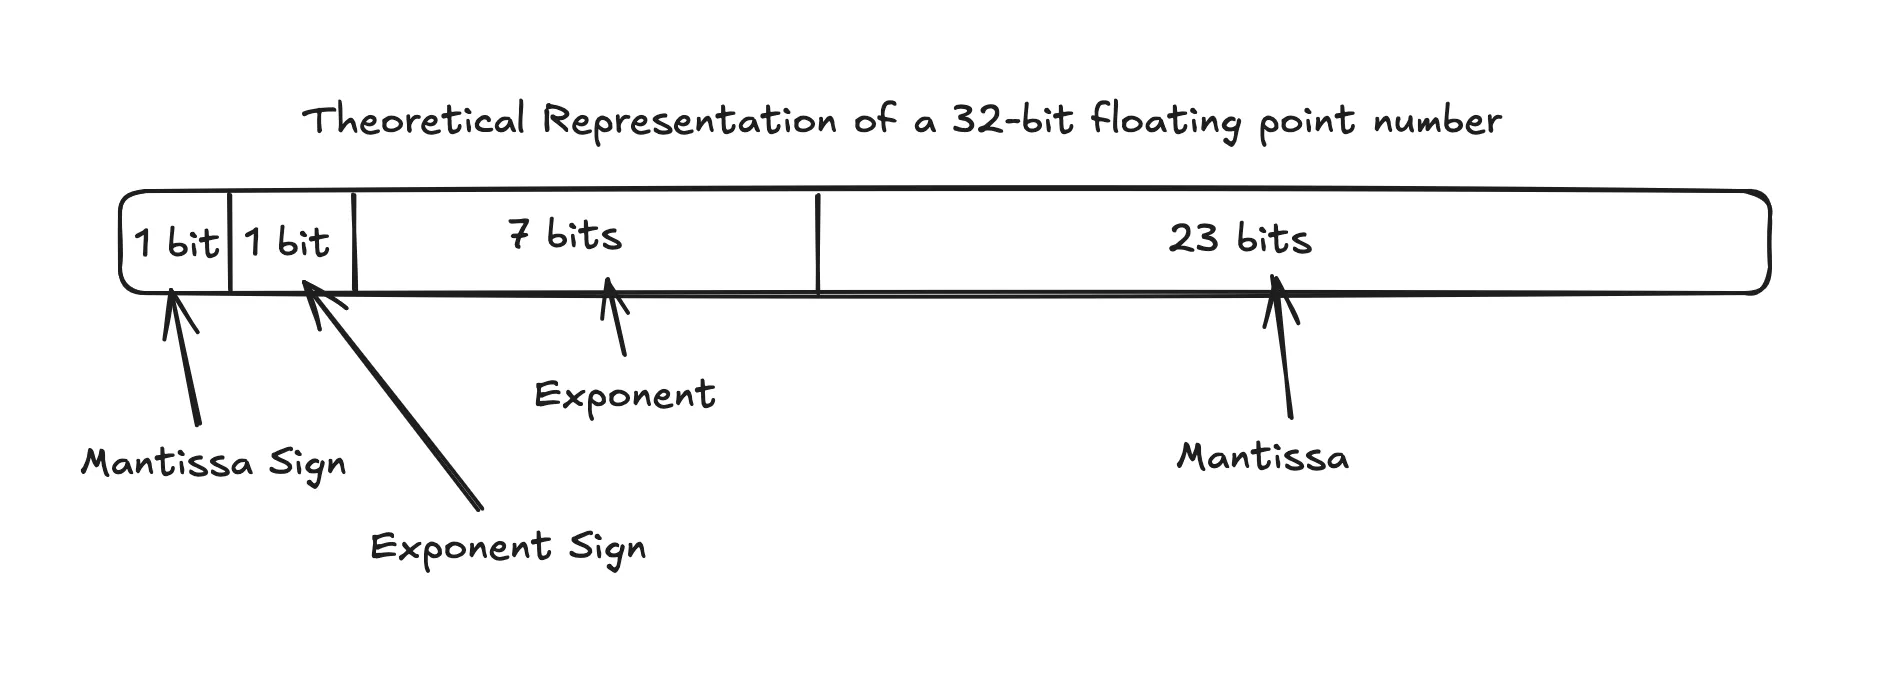
\includegraphics[width=0.8\textwidth]{./assets/fake_ieee754.png}
  \caption{Hypothetical Storage Scheme (32-bit)}
\end{figure}

\subsection{Problems with Floating Point}
\noindent
\begin{minipage}{\textwidth}
Because our storage format is finite, the biggest problems we will encounter
are:
\begin{enumerate}
  \item \textbf{bit overflow}: the maximum magnitude of our exponent (in binary)
    is \textbf{127}, so our number can only range from $2^{-127}$ to $2^{+127}$.
  \item \textbf{rounding error}: because our mantissa only has 23 bits of 
    precision, the precision will decrease as our numbers get larger because we 
    use exponentiation to represent the actual number.
\end{enumerate}
\end{minipage}

% Because our storage format is finite, one of the biggest problems we will 
% encounter is \textbf{bit overflow}. The maximum magnitude of our exponent 
% (in binary) is \textbf{127}, so our number can only range from $2^{-127}$ to
% $2^{+127}$. Because our mantissa only has 23 bits of precision, the precision
% will decrease as our numbers get larger because we use exponentiation to 
% represent the actual number.

\subsubsection{Error Example}

Consider the number $2^{25} = 33,554,432$. This number can be represented 
exactly in binary. However, the number $2^{25}+1 = 33,554,433$ cannot be
represented exactly, since it can't fit within the 23 bits of precision available.

From this, we find that all numbers (including fractions) from $2^{25}-1$ 
through $2^{25}+2$ are represented with the same mantissa in binary. Only when 
you reach $2^{25}+3$ does the mantissa change.

\subsubsection{Remarks}

Within IEEE-754-style floating point representation, the
number of representable values within a given exponent is the same, regardless
of the exponent. This may seem obvious, but it's interesting nonetheless. This
comes from the fact that the number of bits in the mantissa is fixed. The
number of representable values is exactly $2\times 2^{23} = 2^{24}$, since each
positive value has a negative counterpart.


\newcommand{\fl}{\operatorname{fl}}

\section{Floating Point Decimal Normalization}

Can we write all real numbers in normalized scientific notation?
\begin{align*}
    732.5051 &\rightarrow +0.7325051 \times 10^{+3} \\
    -0.005612 &\rightarrow -0.5612 \times 10^{-2}
\end{align*}
For $x \in \mathbb{R}$, we can express it as:
\begin{equation*}
    x = \pm r \times 10^{\pm n}, \quad \text{where } \frac{1}{10} \leq r \leq 1.
\end{equation*}

In binary, we write:
\begin{equation*}
    x = \pm q \times 2^{\pm m}, \quad \text{where } \frac{1}{2} \leq q < 1.
\end{equation*}
Here, $q$ is the mantissa and $m$ is the integer exponent.

We limit $r$ and $q$ so that when $k < 1/\text{BASE}$, we can shift the decimal 
place and normalize the number further. When we have $1.x$, we rewrite it 
as $0.x \times \text{base}^1$.

\section{Rounding or Chopping (Sources of Error)}

Given $x = 0.a_1 a_2 \dots a_n a_{n+1} \dots a_m$ using $m$ digits, rounding 
to $n$ places follows:
\begin{itemize}
    \item If $0 \leq a_{n+1} < 5$, then $x = 0.a_1 a_2 \dots a_n$.
    \item If $5 \leq a_{n+1} \leq 9$, then $x = 0.a_1 a_2 \dots (a_n + 1)$.
\end{itemize}

\textbf{Example:}
\begin{align*}
    \text{round}(0.125) &= 0.13, \\
    \text{round}(-0.125) &= -0.13.
\end{align*}

Instead of rounding, truncation follows:
\begin{equation*}
    x = 0.a_1 a_2 \dots a_n.
\end{equation*}

Truncation introduces larger errors but is computationally cheaper than 
rounding.

\section{Error}

We define:
\begin{itemize}
    \item Absolute error: $|p - p^*|$.
    \item Relative error: $\frac{|p - p^*|}{|p|}$.
\end{itemize}
Absolute error is used when magnitude matters, particularly for small values. 
Relative error is preferred when values differ in scale.

\textbf{Example:}
\begin{align*}
    \text{Exact: } & 0.1, \quad \text{Approximate: } 0.099, \\
    \text{Relative Error: } & \frac{|0.1 - 0.099|}{0.1} = 0.01.
\end{align*}

\begin{center}
\begin{tabular}{|c|c|c|}
    \hline
    $t$ & $5 \times 10^{-t}$ & \text{Is error within bound?} \\
    \hline
    0 & 5 & $\checkmark$ \\
    1 & 0.5 & $\checkmark$ \\
    2 & 0.05 & $\checkmark$ \\
    3 & 0.005 & $\times$ \\
    \hline
\end{tabular}
\end{center}

Since $0.01 < 5 \times 10^{-2}$ but not $5 \times 10^{-3}$, we have two 
significant digits.

\section{Computations and Machine Representation}

Let $\fl(x)$ denote the machine representation of $x$. Computations on a 
machine follow:
\begin{equation*}
    \fl(\fl(x) + \fl(y)).
\end{equation*}
Each step introduces an error.

\textbf{Example:}
\begin{align*}
    p &= 0.54617, \quad q = 0.54601, \\
    r &= p - q = 0.00016.
\end{align*}
With 4-digit rounding,
\begin{align*}
    p^* &= 0.5462, \quad q^* = 0.5460, \\
    r^* &= p^* - q^* = -0.0002.
\end{align*}
Relative error:
\begin{equation*}
    \frac{|r - r^*|}{|r|} = 0.25.
\end{equation*}
A high relative error results when subtracting close numbers.

\section{Minimizing Error}

Consider computing $f(x) = \frac{1 - \cos x}{x^2}$ for $\bar{x} = 1.2 \times 10^{-5}$.

With 10-digit rounding:
\begin{align*}
    c &= \fl(\cos \bar{x}) = 0.9999999999, \\
    1 - c &= 0.0000000001.
\end{align*}
This results in a large error.

Using $\cos x = 1 - 2\sin^2(x/2)$:
\begin{equation*}
    f(x) = \frac{1}{2} \left( \frac{\sin(x/2)}{x/2} \right)^2.
\end{equation*}
This provides a more accurate computation.

\textbf{Conclusion:} Avoid subtracting close numbers. Use alternative 
representations like Taylor series or trigonometric identities.


\section{Reducing Roundoff Error}

One way to reduce roundoff error is to minimize the number of floating-point 
operations.

\subsection{Polynomial Evaluation Using Nested Multiplication}

Consider evaluating the polynomial:
\begin{equation*}
    f(z) = 1.01z^4 - 4.62z^3 - 3.11z^2 + 12.2z - 1.99.
\end{equation*}
We can rewrite this expression using nested multiplication:
\begin{align*}
    f(z) &= (1.01z^3 - 4.62z^2 - 3.11z + 12.2)z - 1.99 \\
         &= ((1.01z^2 - 4.62z - 3.11)z + 12.2)z - 1.99 \\
         &= \dots
\end{align*}
By factoring out $z$ as much as possible, we reduce the total number of 
floating-point operations, minimizing error accumulation.

\section{Cancellation Errors}

\subsection{Quadratic Formula and Cancellation Errors}

Consider solving the quadratic equation:
\begin{equation*}
    ax^2 + bx + c = 0.
\end{equation*}
Using the quadratic formula:
\begin{align*}
    x_1 &= \frac{-b + \sqrt{b^2 - 4ac}}{2a}, \\
    x_2 &= \frac{-b - \sqrt{b^2 - 4ac}}{2a}.
\end{align*}

Suppose $b = 600$, $a = c = 1$. The issue arises because $-b$ is close in 
magnitude to $+\sqrt{b^2 - 4ac}$, causing significant cancellation error in 
$x_1$.

\subsection{Reformulating to Reduce Cancellation}

We rationalize the numerator:
\begin{equation*}
    x_1 = \frac{(-b + \sqrt{b^2 - 4ac})}{2a} \times 
          \frac{(-b - \sqrt{b^2 - 4ac})}{(-b - \sqrt{b^2 - 4ac})}.
\end{equation*}

This simplifies to:
\begin{equation*}
    x_1 = \frac{b^2 - (b^2 - 4ac)}{2a(-b - \sqrt{b^2 - 4ac})}.
\end{equation*}
Now, the cancellation error is eliminated. If $b = -600$, the same issue 
occurs with $x_2$, and we apply the same rationalization technique.

\section{Review of Taylor Series}

Taylor’s theorem is fundamental for numerical approximations.

\subsection{Definition of Taylor Series}

Given a function $f(x)$ that is sufficiently smooth on $[a, b]$, we can 
approximate $f(x)$ with a Taylor polynomial $P_n(x)$:
\begin{equation*}
    P_n(x) = f(x_0) + f'(x_0)(x - x_0) + \frac{f''(x_0)}{2!} (x - x_0)^2 + 
             \dots + \frac{f^{(n)}(x_0)}{n!} (x - x_0)^n.
\end{equation*}

Here, $x_0, x \in [a, b]$.

\subsection{Conditions for Taylor Series Expansion}

For $f(x)$ to have a valid Taylor series expansion:
\begin{itemize}
    \item $f \in C^n[a, b]$ (i.e., $f$, $f'$, $f''$, ..., $f^n$ must be continuous).
    \item $f^{(n+1)}$ must exist on $[a, b]$.
\end{itemize}

\subsection{Error in Taylor Approximation}

The error in Taylor series approximation is given by:
\begin{equation*}
    f(x) = P_n(x) + R_n(x),
\end{equation*}
where the remainder term $R_n(x)$ satisfies:
\begin{equation*}
    R_n(x) = \frac{f^{(n+1)}(c)}{(n+1)!} (x - x_0)^{n+1},
\end{equation*}
for some $c \in (x_0, x)$. The approximation is most accurate when $x$ is 
close to $x_0$.

\section{Example: Third-Order Taylor Polynomial for $\sin(x)$}

Find $P_3(x)$ for $f(x) = \sin(x)$ centered at $x_0 = 0$.

\begin{align*}
    P_3(x) &= f(0) + f'(0)(x - 0) + \frac{f''(0)}{2!} (x - 0)^2 + 
             \frac{f'''(0)}{3!} (x - 0)^3 \\
           &= x - \frac{x^3}{6}.
\end{align*}

\subsection{Error Analysis}

The remainder term for $n = 3$ is:
\begin{equation*}
    R_3(x) = \frac{f^{(4)}(c)}{4!} x^4.
\end{equation*}
Since $f^{(4)}(x) = \sin(x)$, we have:
\begin{equation*}
    R_3(x) = \frac{\sin(c)}{24} x^4.
\end{equation*}
For $x = 0.1$:
\begin{equation*}
    |R_3(0.1)| \leq \frac{|\sin(0.1)|}{24} (0.1)^4 < 4.2 \times 10^{-7}.
\end{equation*}
This shows the high accuracy of the Taylor series approximation.

\section{Linear Approximation of $\sqrt{16.1}$}

We approximate $\sqrt{16.1}$ without using the square root algorithm.

\subsection{Solution}
Let $f(x) = \sqrt{x}$ and choose an expansion point $x_0 = 16$, since 
$\sqrt{16} = 4 \in \mathbb{Z}$ is easily computable. Using the first-order 
Taylor approximation:
\begin{equation*}
    f(x_0 + h) \approx f(x_0) + h f'(x_0),
\end{equation*}
where $h = 0.1$.

\subsection{Computation}
\begin{align*}
    f(16) &= \sqrt{16} = 4, \\
    f'(x) &= \frac{1}{2\sqrt{x}}, \quad f'(16) = \frac{1}{8}, \\
    f(16.1) &\approx 4 + 0.1 \times \frac{1}{8} = 4.0125.
\end{align*}
The exact value is $4.01248052955\dots$, with a small truncation error.
Since the machine error is on the order of $10^{-14}$, it is negligible compared 
to the Taylor approximation error.

\section{Algorithm Quantification}

Numerical methods construct a sequence of better approximations, converging to 
a solution $\alpha$.

Given a sequence $\{\alpha_n\}$:
\begin{equation*}
    \lim_{n\to\infty} \alpha_n = \alpha.
\end{equation*}
We quantify convergence speed by analyzing $|\alpha - \alpha_n| \leq c$, where 
$c$ is a target error.

\subsection{Example: Convergence of $\sin(1/n)$}

Consider $\alpha_n = \sin(1/n)$, which converges to $\alpha = 0$ as $n \to \infty$.
We rewrite:
\begin{equation*}
    \lim_{n \to \infty} \sin(1/n) = \lim_{h \to 0} \sin(h),
\end{equation*}
which is easier to analyze. Expanding $\sin(h)$ in a Taylor series:
\begin{equation*}
    \sin(h) = h - \frac{h^3}{3!} + \frac{h^5}{5!} + \dots.
\end{equation*}
For small $h$, $\sin(h) \approx h$, implying:
\begin{equation*}
    |\alpha_n - \alpha| \leq \frac{1}{n}.
\end{equation*}
Thus, $\alpha_n$ converges to $\alpha = 0$ with rate of convergence $O(1/n)$.

\section{Big-O Notation}

For a sequence $\{A_n\}$, if:
\begin{equation*}
    |A_n - A| \leq k |B_n| \quad \text{for sufficiently large } n,
\end{equation*}
where $k$ is a constant, then we say:
\begin{equation*}
    A_n = A + O(B_n).
\end{equation*}

\subsection{Example: $\sin(1/n)$ Convergence}

From before, $|\alpha_n - \alpha| \leq 1/n$, so:
\begin{equation*}
    A_n = \sin(1/n) \text{ converges to } A = 0 
    \text{ with rate of convergence } O(1/n).
\end{equation*}

\subsection{Example: Convergence of $n \sin(1/n)$}

We evaluate:
\begin{equation*}
    \lim_{n \to \infty} n \sin(1/n) = 1.
\end{equation*}
Changing variables, $h = 1/n$, we obtain:
\begin{equation*}
    \lim_{h \to 0} \frac{\sin(h)}{h} = 1.
\end{equation*}
Expanding $\sin(h)/h$ in Taylor form:
\begin{equation*}
    \frac{\sin(h)}{h} = 1 - \frac{h^2}{6} + O(h^4).
\end{equation*}
For small $h$:
\begin{equation*}
    \frac{\sin(h)}{h} - 1 \approx -\frac{h^2}{6},
\end{equation*}
so $\alpha_n$ converges to $\alpha = 1$ with rate $O(1/n^2)$.

\section{Takeaways}

Big-O notation quantifies algorithm efficiency by ignoring constants and focusing 
on convergence trends. Constants vary across systems, so we care about general 
convergence patterns rather than specific values.

\renewcommand{\arraystretch}{1.25} % Adjust row spacing
\setlength{\arraycolsep}{12pt} 

\section{Review}

Why did we expand around $h_0 = 0$?

\quad Because we want to know what happens with $h_0$, choosing $0$ as our 
expansion point makes sense. The Taylor series approximation is more accurate 
the closer you are to your expansion point.

% As $h \to 0$, the Taylor series approximation converges to the function.

\section{Another Example}

Find the rate of convergence of the following $h\to 0$.

\begin{equation*}
  \lim_{h \to 0} \cos h + \frac{1}{2} h^2 = 1
\end{equation*}

$\alpha = 1$

$\alpha_h = cos h + \frac{1}{2} h^2$

\begin{align*}
  \alpha_h - \alpha &= cos h + \frac{1}{2} h^2 - 1\\
  &= 1-\frac{h^2}{2!}+\frac{h^4}{4!} + O(h^6) + \frac{1}{2}h^2 - 1 \\
  &= \frac{h^4}{4!} + O(h^6) \\
  = O(h^4)
\end{align*}

\section{Chapter 6 - Direct methods for solving linear systems}

\subsubsection*{Preface}

In MATH 240, we learned methods for solving linear systems of equations where
our $n \times m$ matrix has few rows and few columns. In Numerical Analysis, we
will learn methods for solving linear systems where our matrix has thousands or
millions of rows and columns.

We will first study methods that give an answer ina  fixed number of steps, 
subject only to roundoff errors. This method only has error from the accumulation
of numerical representation errors.

\subsection{Linear Systems of Equations}

Linear Systems of Equations

\begin{equation*}
  \begin{bmatrix}
    a_{11} x_1 + a_{12} x_2 + \dots + a_{1n} x_n = b_1 \\
    a_{21} x_1 + a_{22} x_2 + \dots + a_{2n} x_n = b_2 \\
    \vdots \\
    a_{n1} x_1 + a_{n2} x_2 + \dots + a_{nn} x_n = b_n
  \end{bmatrix}
\end{equation*}

\subsection{Elementary Row Operations}

\begin{enumerate}
\item Multiply row $i$ by a constant $\lambda \ne 0$, denoted by 
  $\lambda E_i \to E_i$
\item Add a multiple of row $i$ to row $j$, denoted by $E_i + \lambda E_j \to E_i$
\item Interchange rows $i$ and $j$, denoted by $E_i \leftrightarrow E_j$
\end{enumerate}

\subsection{Notes on Gaussian Elimination}

The idea behind \uline{Gaussian Elimination} is to transform the matrix into
a \enquote*{triangular} equivalent matrix problem of the upper triangular
or lower triangular form.

\subsection{Example 1}

\begin{equation*}
  \begin{bmatrix}
  1 & -1 & 2 & -1 & -8\\
  2 & -2 & 3 & -3 & -20\\
  1 & 1 & 1 & 0 & -2\\
  1 & -1 & 4 & 3 & 12\\
  \end{bmatrix}
\end{equation*}

\section{Complexity of Gaussian Elimination}

How does the number of operations change with the size of the matrices?

We can count up the number of multiplications and divisions to go to upper
triangular form.

\begin{equation*}
  \begin{bmatrix}
  * & \dots & * & x_1\\
  \vdots & \ddots & \vdots & \vdots\\
  * & \dots & * & x_n\\
  \end{bmatrix} 
  \to
  \begin{bmatrix}
   * & * & \dots & * & x_1\\
   0 & * &  & \vdots &  \vdots \\
   \vdots & \vdots & & * & x_n \\
   0 & * & \dots & * & x_{n+1} \\
  \end{bmatrix}
\end{equation*}

This proceeds as follows:

Provided $a_{11} \ne 0$, the operation corresponding to 

\begin{equation*}
  E_j - \frac{a_{ji}}{a_{11}} E_i \to E_j
\end{equation*}


\renewcommand{\arraystretch}{1.25} % Adjust row spacing
\setlength{\arraycolsep}{12pt}

\section{Partial Pivoting}

Parital pivoting is the simplest technique to avoid generating massive roundoff
errors in the Gaussian Elimination algorithm.

The idea is to find the largest element beneath the pivot and swap its row with
the pivot row.

Parital pivoting is sufficient for most linear systems. However, it can be
inadequate for certain problems.

\subsection{Example}

Consider the linear system:

\quad $E_1: 30.00x_1 + 591400x_2 = 491700$

\quad $E_2: 5.291x_1 - 6.130x_2 = 46.78$

No row exchanges are carried out during partial pivoting.

Now, the multiplier is $m_{21} = \frac{5.291}{30.000} = 0.1764$ and 
($E_2-m_{21}E_1 \to E_1$) gives the system

\quad $30.00x_1 + 591400x_2 \approx 591700$

\quad $-104300x_1 \approx -104400$


\renewcommand{\arraystretch}{1.25} % Adjust row spacing
\setlength{\arraycolsep}{12pt}

\section{Scaled Partial Pivoting}

We can improve the accuracy of the partial pivoting algorithm if we scale 
coefficients before deciding on row exchanges.

The scaling factor is the largest absolute value of any coefficient in the 
current row. The idea is to select the largest scaled value $a_{ik}/S_i$
corresponding to elements that are below the pivot.

The extra work to apply the partial pivoting algorithm is some constant
times $O(n^2)$.

In rare instances, complete pivoting may be needed, which is $O(n^3)$ extra
work.

\subsection{An excerpt on Time Complexity}

Total cost of partial pivoting is $O(n^3) + O(n^2) = O(n^3)$

Complete pivoting is $O(n^3) + O(n^3) = O(n^3)$

In the end, the dominant term of complete pivoting is $(c_1 + c_2) O(n^3)$, 
which is technically more than $c_1 O(n^3)$ for partial pivoting, but it is
the extra work is insignificant compared to the total work of the actual 
algorithm.

\section{Some Review (Definitions)}

\begin{enumerate}
\item Two matrices $A$ and $B$ are equal if they have the same size and if each
  element $a_{ij}$ in $A$ is equal to $b_{ij}$ in $B$.
\item $A+B$ for two similarly sized matrices $A$ and $B$ is defined as
  the $n \times n$ matrix whose entries are $(a_{ij} + b_{ij})$ for all 
  $i = 1..n \text{ and } j = 1..m$.
\item $\lambda A$ for a scalar $\lambda$ and a matrix $A$ is defined as
  the matrix whose entries are $\lambda a_{ij}$ for all $i = 1..n \text{ and } 
  j = 1..m$.
\end{enumerate}

\section{Determinants}

A very useful concept of linear algebra is the determinant of a matrix. The
determinant of a matrix $A$ is denoted by $\det(A)$ or $|A|$.

Determinants are important, in part, because of the following theorem:

\subsection{Theorem}

The following statements are equivalent for any $n \times n$ matrix $A$.

\begin{enumerate}
  \item $\det(A) \neq 0$
  \item The equatoin $Ax = 0$ has a unique solution $x=0$.
  \item The system $Ax=b$ has a unique solution for any n-dimensional column
    vector $b$.
  \item The matrix $A$ is nonsingular.\\
    i.e. $A^{-1}$ exists.
\end{enumerate}

\subsection{Definition of the Determinant}

The definition of the determinant is somewhat involved:

\begin{enumerate}[label=(\alph*)]
  \item If $A=[a]$, then $\det(A) = a$
  \item If $A$ is some $n \times n$ matrix, the minor $M_{ij}$ of $A$ is the
    determinant of the $(n-1) \times (n-1)$ submatrix of $A$ obtained by 
    removing the $i^{th}$ row and $j^{th}$ column.
  \item The \uline{cofactor} $A_{ij}$ of $A$ associated with $M_{ij}$ is defined
    by $A_{ij} = (-1)^{i+j} \det(M_{ij})$.
  \item The determinant of the $n \times n$ matrix $A$, when $n>1$ is given
    either by 
    \subitem $\det(A) = \sum_{j = 0}^{n} {a_{ij} A_{ij}}$ (Row cofactor expansion) or
    \subitem $\det(A) = \sum_{j = 0}^{n} {a_{ij} A_{ij}}$ (Column cofactor expansion)
\end{enumerate}

\subsection{Complexity of the Determinant Algorithm}

Assume there are no free zero entries in $A$, and you must compute the 
fully expanded determinant of $A$.

\subsubsection{Work (in general) for a 4x4 matrix}

\begin{align*}
&= 4 \times (\text{work to compute } \det(3 \times 3)) \\
&= 4 \times 3 \times (\text{work to compute } \det(2 \times 2)) \\
&= 4 \times 3 \times 2 \times (\text{work to compute } \det(1 \times 1)) \\
&= 4 \times 3 \times 2 \times 1 \\
&= \boxed{4!}
\end{align*}

Which implies that the determinant of a $n \times n$ matrix can be computed
in $O(n!)$ time.

\section{More ways of computing the determinant}

If $A=[a_{ij}]$ is an $n\times n$ matrix that is either upper or lower
triangular form, then $\det(A) = \prod_{i=1}^n a_{ii}$.


\renewcommand{\arraystretch}{1.25} % Adjust row spacing
\setlength{\arraycolsep}{12pt}

\section{LU-Decomposition}

Suppose that we wanted to solve the system

\begin{equation*}
  Ax = b_k \qquad A \in \mathbb{R}^{n \times n}
\end{equation*}

for several different $b_k \in \mathbb{R}^n$. 

This type of matrix problem arises frequently in initial value problems. If we
apply Gaussian Elimination to solve the system, then $O(n^3)$ operations are
required for each $b_k$. On the other hand, suppose we could factor $A$ into
the form $A = LU$ where $L$ is lower triangular and $U$ is upper triangular.

Then, we can let $y=Ux\implies Ly = b_k$, and solving for $y$ via forward
substitution is $O(n^2)$ operations.

Next, we have to solve for $Ux=y$ via backward substitution, which is also 
$O(n^2)$ operations.

The total number of operations is $O(n^2) + O(n^2) = O(n^2)$, which is much
better than the $O(n^3)$ operations required for Gaussian Elimination.

Finding $L$ and $U$ is $O(n^3)$ requires $O(n^3) + O(n^3)$ operations
\textbf{HOWEVER}, by doing this expensive operation once, we can save a lot of
operations when there are many $b_k$.

\subsection{LU-Factorization}

We will proceed to derive this LU-factorization using Gaussian Elimination.

Example:

\begin{equation*}
  \begin{bmatrix}
    2 & -2 & 3\\
    6 & -7 & 14\\
    4 & -8 & 39\\
  \end{bmatrix}
  \begin{bmatrix}
    u\\
    v\\
    w\\
  \end{bmatrix}
  =
  \begin{bmatrix}
    1\\
    5\\
    14\\
  \end{bmatrix}
\end{equation*}

We want to zero out entries below the pivot element $a_{11}$ in the first row.
So we want to take $E_2-3E_1 \to E_2$. This same effect can be obtained by
multiplying $A$ by the elementary matrix $E_{21}$.

\begin{equation*}
  \begin{bmatrix}
    1 & 0 & 0\\
    -3 & 1 & 0\\
    0 & 0 & 1\\
  \end{bmatrix}
  \begin{bmatrix}
    2 & -2 & 3\\
    6 & -7 & 14\\
    4 & -8 & 39\\
  \end{bmatrix}
  =
  \begin{bmatrix}
    2 & -2 & 3\\
    0 & -1 & 5\\
    4 & -8 & 30\\
  \end{bmatrix}
\end{equation*}

An elementary matrix is equal to the edentity matrix except for one nonzero
entry off of the main diagonal.

Now we want to zero out the remaining entry below the pivot.

This can be done by taking $E_3-2E_1 \to E_3$ or by left-multiplying $A$ by the
elementary matrix $E_{31}$.

\begin{equation*}
  \begin{bmatrix}
    1 & 0 & 0\\
    0 & 1 & 0\\
    -2 & 0 & 1\\
  \end{bmatrix}
  \begin{bmatrix}
    2 & -2 & 3\\
    0 & -1 & 5\\
    4 & -8 & 30\\
  \end{bmatrix}
  =
  \begin{bmatrix}
    2 & -2 & 3\\
    0 & -1 & 5\\
    0 & -4 & 24\\
  \end{bmatrix}
\end{equation*}

To obtain an upper triangular system, we would finally zero out the remaining
entry below the pivot in $E_2$, taking $E_3-4E_2 \to E_3$. Or, we can left
multiply by the elementary matrix $E_{32}$.

\begin{equation*}
  \begin{bmatrix}
    1 & 0 & 0 \\
    0 & 1 & 0 \\
    0 & -4 & 1
  \end{bmatrix}
  \begin{bmatrix}
    2 & -2 & 3 \\
    0 & -1 & 5 \\
    0 & -4 & 24
  \end{bmatrix}
  =
  \begin{bmatrix}
    2 & -2 & 3 \\
    0 & -1 & 5 \\
    0 & 0 & 4
  \end{bmatrix}
\end{equation*}

Notice that $E_{32}E_{31}E_{21}A$ is upper triangular.

Set $U=E_{32}E_{31}E_{21}$ and $L=A$.

Now $E_{32}^{-1}E_{31}^{-1}E_{21}^{-1}U=L$.

To find the inverses of elementary matrices, we have to recall their meaning.

For example, $E_{21} = \begin{bmatrix}
1 & 0 & 0\\
-3 & 1 & 0\\
0 & 0 & 1\\
\end{bmatrix}$ subtracts $3$ times the first row from the second.

The inverse will need to add 3 times the first row to the second.

\begin{equation*}
  \implies (E_{21})^{-1} = \begin{bmatrix}
    1 & 0 & 0\\
    3 & 1 & 0\\
    0 & 0 & 1\\
  \end{bmatrix}
\end{equation*}

Which costs $O(1)$ operations to flip the sign of the single entry.

Furthermore, notice that 

$L \cong E_{21}^{-1}E_{31}^{-1}E_{32}^{-1}$

\begin{align*}
  &= \begin{bmatrix}
  1 & 0 & 0\\
  3 & 1 & 0\\
  0 & 0 & 1\\
  \end{bmatrix} \begin{bmatrix}
  1 & 0 & 0\\
  0 & 1 & 0\\
  2 & 0 & 1\\
  \end{bmatrix} \begin{bmatrix}
  1 & 0 & 0\\
  0 & 1 & 0\\
  0 & 4 & 1\\
  \end{bmatrix} \\
  &= \begin{bmatrix}
  1 & 0 & 0\\
  3 & 1 & 0\\
  2 & 4 & 1\\
  \end{bmatrix}
\end{align*}

So the matrix multiplication can be performed by putting the nonzero offdiagonal
elements of the elementary matrices intot he appropriate positions in the matrix
$L$.

This means that the matrix $L$ is easily constructed during the Gaussian
Elimination process just by storing the multipliers.

We conclude that

\begin{equation*}
  \underset{A}{
    \begin{bmatrix}
      2 & -2 & 3\\
      6 & -7 & 14\\
      4 & -8 & 30\\
    \end{bmatrix}
  }
  =
  \underset{L}{
    \begin{bmatrix}
      1 & 0 & 0\\
      3 & 1 & 0\\
      2 & 4 & 1\\
    \end{bmatrix}
  }
  \underset{U}{
    \begin{bmatrix}
      2 & -2 & 3\\
      0 & -1 & 5\\
      0 & 0 & 4\\
    \end{bmatrix}
  }
\end{equation*}


\renewcommand{\arraystretch}{1.25} % Adjust row spacing
\setlength{\arraycolsep}{12pt}

\section{LU Decomposition (contd.)}

THM: If Gaussian elimination can be performed without row exchanges, then the
matrix $A$ has a unique $LU$ factorization where $L$ is lower triangular and
with all diagonal entries equal to $1$ and $U$ is an upper triangular matrix.

Once the matrix factorization is complete, the solution to

\begin{equation*}
  LUx = b
\end{equation*}

is found by first setting 

\begin{equation*}
  y=Ux
\end{equation*}

then determining the vector $y$ from $Ly=b$ using forward substitution. The
variable $x$ is found from $Ux=y$ using backward substitution.

Notice: in the theorem, \textbf{we need to be able to perform Gaussian
Elimination without row exchanges}. This means that we can't use row
exchanges to solve the system.

\section{Matrix Factorization}

If $A$ is any nonsingular matrix, $Ax=b$ can be solved by Gaussian Elimination
with the possibility of row exchanges. If we can find the row interchanges
required to solve the system by Gaussian Elimination, then we can re-arrange
the equations in an order that would ensure that no row interchanges are
required.

$\implies$ There is a rearrangement of the equations that permits Gaussian
Elimination without row exchanges.

But WHY does the rearrangement of the equations break LU decomposition?

\section{Permutation Matrix}

An $n\times n$ permutation matrix $P$ is obtained by rearranging the rows of
the identity matrix. This gives a matrix with precisely one nonzero entry in
each row and column. The nonzero entries are all $1$'s.

On the other hand, multiplying $A$ on the right by $P$ will exchange the
second and third \textbf{columns} of $A$.

We will be using the following two properties of permutation matrices:

\begin{enumerate}
  \item If $K_1,...,K_n$ is a permutation of the integers $1,...,n$, and the
    permutation matrix $P=[p_{ij}]$ is defined by 

    \qquad $p_{ij}=\begin{cases}
      1 & i=K_j\\
      0 & \text{otherwise}
    \end{cases}$

    Then, $PA$ permutes the rows of $A$ according to (BIGASS MATRIX MISSING HERE)
    data from chapter6-part2.pdf page 3.
  \item If $P$ is a permutation matrix, then $P^{-1}$ exists and $P^{-1}=P^T$
\end{enumerate}

Now our approach will be to left multiply the system

\begin{equation*}
  Ax=b
\end{equation*}

by the appropriate permutiation matrix $P_1$ so that the system

\begin{equation*}
  (PA)x=Pb
\end{equation*}

can be solved without row exchanges. Then $PA$ can be factorized into

\begin{equation*}
  PA=LU
\end{equation*}

This tells us that

\begin{align*}
  P^{-1}LUx &= b \\
  LUx &= Pb
\end{align*}

which can be solved rapidly for $x$.




\renewcommand{\arraystretch}{1.25} % Adjust row spacing
\setlength{\arraycolsep}{12pt}

\section{Speical Types of Matrices}

\noindent
Where can Gauassian Elimination be performe without row exchanges?

\subsection{Strictly Diagonally Dominant Matrices}

\textbf{Def.} An $n\times n$ matrix $A$ is \uline{strictly diagonally dominant} 
if 

\begin{equation*}
  |a_{ii}| > \sum_{j=1; j\ne i}^{n} |a_{ij}| \text{ for all } i=1,\dots,n
\end{equation*}

\subsubsection*{Example}

\begin{equation*}
  \begin{bmatrix}
  3h & h & -h\\
  4 & 10 & 4\\
  1 & 1 & -3\\
  \end{bmatrix}
\end{equation*}

This matrix is strictly diagonally dominant when $h\ne 0$.

\subsubsection{Thm. 1}

A strictly diagonally dominant matrix $A$ is nonsingular.

\subsubsection{Thm. 2}

Let $A$ be a strictly diagonally dominant matrix. Then Gaussian Elimination
can be performed on any linear system of the form $Ax=b$ to obtain its 
unique solution without row or column interchanges, and the computations
are stable to the growth of roundoff error.

\subsection{Symmetric, Positive Definite Matrices}

\textbf{Def.} A matrix $A$ is \uline{positive definite} if

\begin{equation*}
  \forall x\ne 0 (x^T A x > 0)
\end{equation*}

\subsubsection*{Example}

Find all values of $\alpha$ for which the matrix

\begin{equation*}
  A = 
  \begin{bmatrix}
    1 & 0 & -1\\
    0 & 1 & 1\\
    -1 & 1 & \alpha\\
  \end{bmatrix}
\end{equation*}

is positive definite.

\textbf{Ans.} 

\begin{align*}
  x^T Ax &= 
  \begin{bmatrix}
  x_1 & x_2 & x_3
  \end{bmatrix}
  \begin{bmatrix}
    1 & 0 & -1\\
    0 & 1 & 1\\
    -1 & 1 & \alpha\\
  \end{bmatrix}
  \begin{bmatrix}
  x_1 \\ x_2 \\ x_3
  \end{bmatrix}\\
         &= x_1^2 + x_2^2 + \alpha x_3^2 - 2x_1x_3 + 2x_2x_3 \\
         &= (x_1 - x_3)^2 + (x_2 + x_3)^2 + (\alpha - 2) x_3^2 
\end{align*}

A is positive definite $\iff \alpha > 2$.

Some necessary conditions for an $n\times n$ matrix to be positive definite u
include:

\begin{enumerate}[label=(\alph*)]
\item $A$ is nonsingular
\item $a_{ii} > 0$ for each $i=i...n$ 
\item ???
\item $(a_{ij})^2 < a_{ii} a_{jj}$ for each $i\ne j$
\end{enumerate}

\textbf{HOWEVER:} These are not sufficient conditions for positive definiteness.
they are necessary but not sufficient.

We would like necessary and sufficient conditions for a matrix to be positive
definite.

\subsection{Leading Principle Submatrices}

A \uline{leading principle submatrix} of a matrix $A$ is a matrix of the form

\begin{equation*}
  A_k = \begin{bmatrix}
    a_{11} & a_{12} & \dots & a_{1n}\\
    a_{21} & a_{22} & \dots & a_{2n}\\
   \vdots&  &  & \\
   a_{k1} & a_{k2} & \dots & a_{kn}\\
  \end{bmatrix}
\end{equation*}

for some $1 \leq k \leq n$.

Based on this definition, we have the following theorem:

\subsubsection{Thm. 3}

A symmetrix matrix $A$ is positive definite if and only if each of its leading
principle submatrices has a positive determinant.

As it turns out, we don't need to carry out row exchanges when Gaussian
Elimination is used on a symmetric, positive definite matrix.

\subsubsection{Thm. 4}

A symmetric matrix $A$ is positive definite if and only if Gaussian Elimination
withour row exchanges can be performed on the linear system $Ax=b$ with
all the pivot elements positive. Moreover, in this case, the computations are
stable with respect to the growth of roundoff error.

\textbf{Corollary:} The matrix $A$ is symmetric positive definite if and only if
$A$ can be factored in the form $LDL^T$ where $L$ is lower triangular with $1$'s
on its diagonal and $D$ is a diagonal matrix with positive diagonal entries.

A modification of the $LU$ factorization algorithm can be made to factor a
symmetric positive definite matrix into the form

\begin{equation*}
  A = LDL^T
\end{equation*}

This $LDL^T$ factorization only requires $\frac{n^3}{6}+n^2 - \frac{7n}{6}$ 
multiplications/divisions, and $\frac{n^3}{6}-\frac{n}{6}$ additions/subtractions.
This is only half the number of operations as $LU$ factorization.

A version of this algorithm can also be constructed for matrices that are
symmetric but not positive definite.

\textbf{Corollary 2:} The matrix $A$ is positive definite if and only if $A$ can
be factored int he form $LL^T$ where $L$ is lower triangular with nonzero
diagonal entries. Once again, a modification of the $LU$ factorization algorithm
can be made. This method, called \uline{Choleski's Algorithm}, factors a
symmetric positive definite matrix into the form

\begin{equation*}
  A = LL^T
\end{equation*}

Choleski's Algorithm only requires $\frac{n^3}{6} + \frac{n^2}{2} - \frac{2n}{3}$
multiplications/divisions, and $\frac{n^3}{6}-\frac{n}{6}$ additions/subtractions,
which is even less than the $LDL^T$ factorization. However, for small $n$,
Choleski's Algorithm may be slower because it requires $n$ square roots to
be computed.

\subsection{Band Matrices}

Another important class of matrices that arise in a wide variety of applications
are \uline{band matrices}. A band matrix is a matrix of the form
 

\renewcommand{\arraystretch}{1.25} % Adjust row spacing
\setlength{\arraycolsep}{12pt}

\section{More Special Matrices}

\subsection{Band Matrices}
Another important class of matrices that arise in a wide variety of 
applications are called band matrices. These matrices concentrate all their 
nonzero entries about the diagonal.

\subsubsection{Definition}
An $n \times n$ matrix is called a band matrix if there exist integers $p$ and
$q$ such that $1 < p, q < n$ having the property that $a_{ij} = 0$ whenever
$i + p \leq j$ or $j + q \leq i$.

The bandwidth of a band matrix is defined as $w = p+q-1$. We subtract 1 from 
our count because we do not want to double count the diagonal.

We will focus on the important case of tridiagonal matrices, which are band 
matrices with $p = q = 2$, i.e., the matrix is tridiagonal if the nonzero 
entries are on the main diagonal and the diagonals above and below the main 
diagonal.

Suppose $A$ can be factored into the triangular matrices $L$ and $U$. Suppose
that the matrices can be found in the form:

\[
L = \begin{bmatrix}
    l_{11} & 0 & \dots & 0 \\
    l_{21} & l_{22} & & \\
    & & \ddots & \\
    0 & \dots & l_{n,n-1} & l_{nn}
\end{bmatrix}
\]

\[
U = \begin{bmatrix}
    u_{11} & u_{12} & \dots & u_{1n} \\
    0 & u_{22} & \dots & u_{2n} \\
    & & \ddots & \\
    0 & 0 & \dots & u_{nn}
\end{bmatrix}
\]

The zero entries of $A$ are automatically generated by $LU$. Multiplying
$A = LU$, we also find the following conditions:

1. \[ a_{11} = l_{11}, \quad a_{i,i-1} = l_{i,i-1}, \quad i = 2,3,\dots,n \]
2. \[ a_{ii} = l_{i,i-1} u_{i-1,i} + l_{ii}, \quad i = 2,3,\dots,n \]
3. \[ a_{i,i+1} = l_{ii} u_{i,i+1}, \quad i = 1,2,\dots,n-1 \]

This system is straightforward to solve: (1) gives us $l_{11}$ and the 
off-diagonal entries of $L$. (2) and (3) are used alternately to obtain 
the remaining entries of $L$ and $U$. This solution technique is often referred
to as \textbf{Crout Factorization}.

If we count up the number of operations, we find:

- $(5n - 4)$ multiplications/divisions
- $(3n - 3)$ additions/subtractions

Crout Factorization can be applied to a matrix that is positive definite or one
that is strictly diagonally dominant. See the text for another general case 
where it can be applied.


\renewcommand{\arraystretch}{1.25} % Adjust row spacing
\setlength{\arraycolsep}{12pt}

\section{Iterative Techniques in Matrix Algebra}

We are interested in solving large linear systems $Ax=b$.

Suppose the matrix $A$ has a high $(>99.9\%)$ sparsity, i.e., most of the
entries are zeros. We would like to take advantage of this spare structure to
reduce the amount of computational work required. Unfortunately, Gaussin
Elimination is often unable to take advantage of the sparse structure. For this
reason, we consider \uline{iterative techniques}.

\section{Vector Norms}

To estimate how well a particular iterative technique approximates
the true solution, we will need some measurement of distance. This motivates
the notion of the vector norm.

\textbf{Def.} A vector norm on $\mathbb{R}^n$ is a function $||\cdot||$ from
$\mathbb{R}^n \to \mathbb{R}^n $ satisfying the following properties:

\begin{itemize}
  \item $||x|| \geq 0$ for all $x \in \mathbb{R}^n$
  \item $||x|| = 0 \iff x = \mathbf{0}$
  \item $||\alpha x|| = |\alpha| ||x||$ for all $\alpha \in \mathbb{R}$ and
    $x \in \mathbb{R}^n$
  \item $||x+y|| \leq ||x|| + ||y|| $ for all $x,y \in \mathbb{R}^n$
\end{itemize}

\textbf{Def. 2.} The $l_2$ or Euclidean norm of the vector $x$ is given by
\begin{equation*}
  ||x||_2 = \left\{ \sum_{i = 1}^{n}  x_i^2 \right\}^{1/2}
\end{equation*}

This represents the usual notion of distance.

\textbf{Def. 3.} The infinity or max norm of a vector $x$ is given by

\begin{equation*}
  ||x||_\infty = \max_{i=1}^n |x_i|
\end{equation*}

\textbf{Def. 4.} If $x,y \in \mathbb{R}^2$, then the $l_2$ distance between
$x$ and $y$ is given by

\begin{equation*}
  ||x-y||_2 = \left\{ \sum_{i=1}^{n} (x_i-y_i)^2 \right\}^{1/2}
.\end{equation*}

and the $l_\infty$ distance between $x$ and $y$ is given by

\begin{equation*}
  ||x-y||_\infty = \max_{i=1}^n |x_i-y_i|
.\end{equation*}

\section{Sequences?}

Iterative techniques generate a sequence of vectors.

\textbf{Def.} A sequence $\left\{ x^k \right\}_{k=1}^\infty$ of vectors in
$\mathbb{R}^n$ is said to converge to $x$ with respect to the norm $||\cdot||$
if, given any $\epsilon > 0$, there exists an integer $N('\epsilon)$ such that

\begin{equation*}
  ||x^{(k)} - x|| < \epsilon \text{ for all } k \geq N
\end{equation*}

*The notation $N('\epsilon)$ is used to emphasize that $N$ is dependent on 
$\epsilon$, however, $N$ is not a function of $\epsilon$.*

\subsection{Thm.}

The sequence of vectors $\left\{ x^k \right\}$ converges to $x$ in $\mathbb{R}^n $
with respect to $||\cdot||_\infty$ if and only if 
$\lim_{k \to \infty} x_i^{(k)} = x_i$. for each $i$.

\subsection{Thm. 2}

For each $x\in \mathbb{R}^n $

\begin{equation*}
  ||x||_\infty \leq ||x||_2 \leq \sqrt{n} ||x||_\infty
\end{equation*}

This theorem relates the infinity norm to the Euclidean norm, which is very 
useful in the context of iterative techniques.


% \setlength{\arraycolsep}{12pt}
%
% \newcommand{\defn}{\textbf{Def.}\xspace}
% \newcommand{\thm}{\textbf{Thm.}\xspace}
% \newcommand{\ex}{\textbf{Ex.}\xspace}
% \renewcommand{\arraystretch}{1.25} % Adjust row spacing
\subsubsection*{Example 1}

Prove that $x^{(k)} = \left(\frac{1}{k}, 1+e^{1-k}, -\frac{2}{k^2}\right)^t$
is convergent w.r.t. $||\cdot||_2$.

We know $0 \leq ||x^{(k)}-x||_2 \leq \sqrt{3}||x^{(k)}-x||_{\infty}$

\begin{eqnarray*}
  \lim_{k \to \infty} ||x^{(k)}-x||_{\infty} = 0 \implies \lim_{k \to \infty}
  ||x^{(k)}-x||_2 = 0 \\
\end{eqnarray*}

So, $\left\{x^{(k)}\right\}$ is convergent to $x$ w.r.t. $||\cdot||_2$.

It can be shown that \uline{all} norms on $\mathbb{R}^n $ are equivalent with
respect to convergence.

i.e. If $||\cdot||_a$ and $||\cdot||_b$ are norms on $\mathbb{R}^n$, and
$\left\{x^{(k)}\right\}_{k=1}^{\infty}$ has the limit $x$ with respect to
$||\cdot||_a$, then $\left\{x^{(k)}\right\}_{k=1}^{\infty}$ also has the limit
$x$ with respect to $||\cdot||_b$.

\section{Matrix Norms}

\textbf{Def.} A \uline{matrix norm} on the set of all $n \times n$ matrices 
$(R^{n \times n})$ is a real-valued function $||\cdot||$ defined on this set
satisfying for all $n \times n$ matries $A$ and $B$ and all real numbers
$\alpha:$

\begin{enumerate}
  \item $||A|| \geq 0$
  \item $||A|| = 0 \iff A=0$
  \item $||\alpha A|| = |\alpha| ||A||$
  \item $||A+B|| \leq ||A|| + ||B||$
  \item $||AB|| \leq ||A|| ||B||$
\end{enumerate}

\textbf{Def.} A distance between two $n\times n$ matrices $A$ and $B$ is

\begin{equation*}
  ||A-B||
\end{equation*}

\subsection{Thm.}

If $||\cdot||$ is a vector norm on $\mathbb{R}^n $, then 

\begin{equation*}
  ||A|| = \max_{||x||=1} ||Ax||.
\end{equation*}

is a matrix norm.

This is called the natural or induced matrix norm associated with the vector
norm.

The following result gives a bound on the value of $||Ax||$:

\subsection{Thm.}

For any vector $x\ne 0$, matrix $A$, and any natural norm $||\cdot||$, we have

\begin{equation*}
  ||Ax|| \leq ||A|| \cdot ||x||.
\end{equation*}

\subsubsection{Notes on the Infinity Norm}

The infinity norm is defined as

\begin{equation*}
  ||x||_\infty = \max_{i} |x_i|
\end{equation*}

So, it's the maximum absolute value of every entry in $x$.

\textbf{Example:} $x=\left(\begin{array}{c}
  1 \\
  -2 \\
  1.5 \\
\end{array}\right)$

$||x||_\infty = 2$

Because the largest element (in magnitude) is $-2$.

\section{Computing the Infinity Norm and the 1-Norm}

Computing the $\infty$-norm of a matrix is straightforward:

\subsection{Thm.}

If $A=(a_{ij})$ is a $n \times n$ matrix, then

\begin{equation*}
  ||A||_\infty = \max_{1\leq i \leq n} \sum_{j=1}^n |a_{ij}|
\end{equation*}

\textbf{Example:}

Find 

\begin{equation*}
  \left|\left| \begin{bmatrix}
  2 & -1 & 0\\
  -1 & 2 & -1\\
  0 & -1 & 2\\
  \end{bmatrix} \right|\right|_\infty
\end{equation*}

\begin{align*}
  \sum_{j=1}^n |a_{1j}| &= |2| + |-1| + |0| = 3 \\
  \sum_{j=1}^n |a_{2j}| &= |-1| + |2| + |-1| = 4 \\
  \sum_{j=1}^n |a_{3j}| &= |0| + |-1| + |2| = 3 \\
  \implies ||A||_\infty &= \max\{3, 4, 3\} = 4
\end{align*}

\pagebreak
\subsection{Visualizing the Infinity Norm}

Images courtesy of ChatGPT. I got really confused by the concept of the
infinity norm, so I asked the bot for help.

\begin{figure}[h]
  \centering
  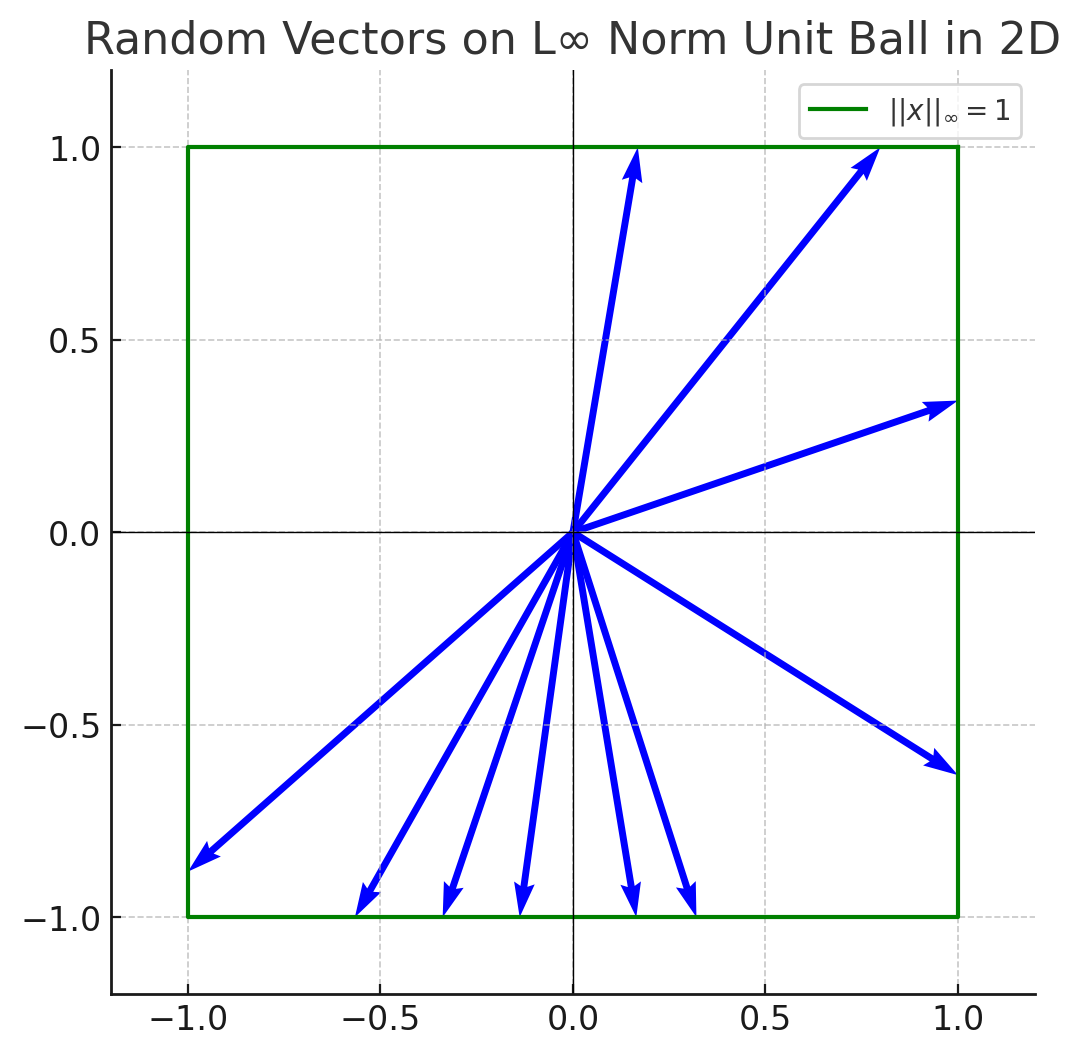
\includegraphics[width=0.8\textwidth]{./assets/infinity_norm.png}
  \caption{Visualizing the Infinity Norm}
\end{figure}

So the reason why the infinity norm, visualized this way,
looks like a square, is because the equation $||x||_\infty = 1$ is equivalent 
to saying \enquote{the set of all vectors $x$ such that the the largest 
component magnitude of the vector is 1}. Meaning this is the set of all vectors
that have $x=1$ or $y=1$

\section{Eigenvalues and Eigenvectors} % spend time reviewing this

To calculate the $l_\infty$-norm of a matrix, we did not need to directly
appy the definition. This is also true for the $l_2$-norm, however, we will need
to introduce eigenvalues and eigenvectors to apply this technique.

First we will need the following definition:

\noindent
\textbf{Def.} If $A$ is a square matrix, the polynomial defined by

\begin{equation*}
  p(\lambda) = \det(A-\lambda I)
\end{equation*}

\noindent
\hangindent=0.5cm
\hangafter=0
is called the \uline{characteristic polynomial} of $A$. It is easily shown that
$p$ is an $n^{th}$ degree polynomial.

Now we can introduce eigenvalues and eigenvectors.

\noindent
\hangindent=0.5cm
\hangafter=1
\textbf{Def.} If $p$ is the characteristic polynomial of the matrix $A$, the
zeros of $p$ are called eigenvalues, or characteristic values of $A$. If $
\lambda$ is an eigenvalue of $A$ and $x\ne 0$ has the property that 
$(A-\lambda I)x = 0$ then $x$ is called an eigenvector, or characteristic
vector, of $A$ corresponding to the eigenvalue $\lambda$.

\noindent\rule{\linewidth}{0.5pt}

The professor does not specifically discuss eigenvectors and eigenvalues in the
context of Numerical Analysis, but they will be important for future problems.
He also does not mention how to compute them.

However, he did suggest that we review how to compute them by hand and study 
the related theorems.

\section{Finding the $l_2$-norm of a matrix}

\defn The spectral radius $\rho(A)$ of a matrix $A$ is defined as

\begin{equation*}
  \rho(A) = \max \left|\lambda\right| \text{ where } \lambda \text{ is an eigenvalue of } A
\end{equation*}

\ex

\begin{equation*}
  \rho(\begin{bmatrix}
  2 & 1 & 0\\
  1 & 2 & 0\\
  0 & 0 & 3\\
  \end{bmatrix}) = \max \left\{ |3|, |3|, |1| \right\} = 3
\end{equation*}

And now, we can consider the following:

\pagebreak
\thm If $A$ is a $n \times n$ matrix, then

\begin{enumerate}
  \item $||A||_2 = \sqrt{\rho(A^T A)}$
  \item $\rho(A) \leq ||A||$ for any natural norm $||\cdot||$
\end{enumerate}

My editor broke in the middle so you should look at the Chapter 7 PDF notes
for the proofs and examples. The end of this section is around page 19 of 
the PDF. (35.13)


When we use iterative matrix techniques, we want to know when powers of a 
matrix become small.

\defn We call an $n \times n$ matrix $A$ convergent if 

\begin{equation*}
  \lim_{k\to\infty} \left(A^k\right)_{ij} = 0, \text{ for all } i,j
\end{equation*}

\ex Consider $A=\begin{bmatrix}
\frac{1}{2} & 0\\
16 & \frac{1}{2}\\
\end{bmatrix}$

\begin{align*}
  A^2 &= 
  \begin{bmatrix}
    \frac{1}{4} & 0 \\
    16 & \frac{1}{4}
  \end{bmatrix} \\
  A^3 &= 
  \begin{bmatrix}
    \frac{1}{8} & 0\\
    12 & \frac{1}{8}\\
  \end{bmatrix}\\
  A^4 &= 
  \begin{bmatrix}
    \frac{1}{16} & 0\\
    8 & \frac{1}{16}\\
  \end{bmatrix} \\
  A^k &= 
  \begin{bmatrix}
    \frac{1}{2^k} & 0\\
    P_k & \frac{1}{2^k}\\
  \end{bmatrix}
\end{align*}

where $P_k = \begin{cases}
16 & k=1\\
\frac{16}{2^{k-1}} + \frac{1}{2}P_{k-1} & k>1
.\end{cases}$

Since $\lim_{k\to\infty} P_k = 0$, we also know that $\lim_{k\to\infty} P_k = 0$.
$\therefore A$ is a convergent matrix.

Notice that this convergent matrix has a spectral radius (see Lecture 12 notes
, page 5) less than 1.

This generalizes:
\pagebreak

\thm The following statements are equivalent:

\begin{enumerate}
  \item $A$ is a convergent matrix.
  \item $\rho(A) < 1$
  \item $\lim_{n\to\infty} A^n x = 0$ for every $x$
  \item $\lim_{n\to\infty} \left|\left|A^n\right|\right| = 0$ for all natural
    norms $||\cdot||$
\end{enumerate}

Iterative techniques convert the system $Ax=b$ into an equivalent system of
the form $x=Tx+c$ where $T$ is a fixed matrix and $c$ is a vector. An initialv
vector $x^{(0)}$ is chosen, and then a sequence of approximate solution vectors
is generated:

\begin{equation*}
  x^{(k)} = Tx^{(k-1)} + c
\end{equation*}

Iterative techniques are rarely used in very small systems 
(i.e. when $n^3$ is small). In these cases, iterative techniques may be slower 
since they require several iterations to obtain the desired accuracy.

\uline{\textbf{IDEA:}} It is possible to \enquote{split} the matrix $A:$

\begin{align*}
  Ax&=b \\
  \left[M+(A-M\right]x &= b \\
  Mx &= b+(M-A)x \\ 
  x &= (I-M^{-1}A)x + M^{-1}b 
\end{align*}

Iteration becomes 

\begin{equation*}
  x^{(k+1)} = (I-M^{-1}A)x^{(k)} + M^{-1}b
\end{equation*}

We set $T\cong I-M^{-1}A$ (the amplification matrix) and $c\cong M^{-1}b$.

\begin{equation*}
  x^{(k+1)} = Tx^{(k)} + c
\end{equation*}

How do we choose $M$?

We want:

\begin{enumerate}
\item $M$ easy to \enquote{invert}
\item M \enquote{close to $A$} in the sense that $\rho(T)$ is small.
\end{enumerate}

\ex Let $M=D=\begin{bmatrix}
  a_{11} & 0 & 0\\
0 & \ddots & 0\\
0 & 0 & a_{nn}\\
\end{bmatrix}$

This gives the \uline{Jacobi Iterative Method}.

In the text's notation,

\begin{equation*}
  A=D-L-U
\end{equation*}

Where $D$ is diagonal, $L$ is lower triangular, and $U$ is upper triangular.

\begin{align*}
  Ax &= b \\
  (D-L-U)x &= b \\
  Dx &= (L+U)x + b\\
  x &= D^{-1}(L+U)x +D^{-1}b \\
\end{align*}

Which results in the iteration 

\begin{equation*}
  x^{(k+1}) = D^{-1}(L+U)x^{(k)} + D^{-1}b
\end{equation*}

Let $T=D^{-1}(L+U)$ and $c=D^{-1}b$.

\begin{equation*}
  x^{(k+1)} = Tx^{(k)} + c
\end{equation*}

See example in the notes, there are too many matrices to type out in LaTeX.
See \enquote{Chapter 7.pdf} page 27 (7-36.7)

% Click: \href{run:./Chapter 7.pdf#page=27}{Chapter 7.pdf} page 27 (7-36.7)

\subsubsection{Comments on Jacobi's Method}

\begin{equation*}
  x^{(k+1)} = D^{-1}(L+U)x^{(k)} + D^{-1}b
\end{equation*}

\begin{enumerate}
  \item The algorithm requirs $a_{ii} \neq 0$ for $i=1,\dots,n$ If one of the 
    $a_{ii} = 0$, and the system is nonsingular, then a reordering of the 
    equations can be performed so that no $a_{ii} = 0$.
  \item To speed convergence, the equations should be arranged such that
    $|a_{ii}$ is as large as possible.
  \item A possible stopping criterion is to iterate until
    $\frac{||x^{(k)}-x^{(k-1)}||}{||x^{(k-1)}||} \leq \epsilon$
\end{enumerate}

If we write out Jacobi's Method

\begin{equation*}
  x^{(k+1)} = D^{-1}(L+U)x^{(k)} + D^{-1}b
\end{equation*}

we find that

\begin{equation*}
  x_i^{(k+1)} = \frac{\sum_{j=1; j\ne i}^n (-a_{ij}x_j^{(k)}) +b_i}{a_{ii}}
\end{equation*}

Notice that to compute $x_i^{(k+1)}$, the components $x_i^{(k)}$ are used.
But, for $i>1$, $x_1^{(k+1}, x_2^{(k+1)}, \dots, x_n^{(k+1)}$ have already
been computed and are likely better approximations to the actual solutions than

\begin{equation*}
  x_1^{(k)}, x_2^{(k)}, \dots, x_n^{(k)}
\end{equation*}

So it seems reasonable to compute with these most recently computed values.

\ie:

\begin{equation*}
  x_i^{(k+1)} = \frac{-\sum_{j=1}^{i=1}(a_{ij}x_j^{(k+1)} - \sum_{j=i+1}^{n} (a_{ij} x_j^{(k)} +b_i}{a_{ii}}
\end{equation*}

This is called the Gauss-Seidel iterative technique, and it also has a matrix
formulation with $M\cong (D-L):$

\begin{align*}
  Ax &= b \\
  (D-L-U)x &= b \\
  (D-L)x &= Ux+b \\
  x &= (D-L)^{-1}Ux+(D-L)^{-1}b
\end{align*}

$\implies$ iteration becomes

\begin{equation*}
  x^{(k+1)} = (D-L)^{-1}Ux^{(k)} + (D-L)^{-1}b
\end{equation*}

*Notice that $D-L$ is lower triangular. It is invertible $\iff$ each $a_{ii}\ne 0$


\section{Solutions of Nonlinear Systems}

The Basic Problem:

Find a root of $x\in\mathbb{R}$ of an equation of the form $f(x)=0$ for a
given continuous function $f$.

\section{The Bisection Method}

In most cases it is not really possible to solve analytically. We will consider
iterative methods to approximate the solution. Our first method will be the
\uline{Bisection Method}. We must start with an interval $[a, b]$ with 
$f(a)$ and $f(b)$ of opposite signs.

By the intermediate value theorem, there exists a number $c$ in $(a, b)$ such that
$f(c)=0$.

\thm If $f\in C[a,b]$ and $k$ is any number between $f(a)$ and $f(b)$, then
there exists a number $c$ in $(a, b)$ such that $f(c)=k$.

Now set $a_1 = a$ and $b_1 = b$ and let $p_1$ be the midpoint of $[a_1, b_1]$.

\begin{enumerate}
    \item Compute the midpoint:
    \begin{equation*}
        p_1 = \frac{1}{2} (a_1 + b_1)
    \end{equation*}
    
    \item If $f(p_1) = 0$, then we are done. Set $p = p_1$.
    
    \item If $f(p_1)$ and $f(a_1)$ are of opposite signs, then there must exist 
          a root $p \in (a_1, p_1)$ such that $f(p) = 0$. Set $a_2 = a_1$ and 
          $b_2 = p_1$.
    
    \item Otherwise, if $f(p_1)$ and $f(b_1)$ are of opposite signs, then there 
          must exist a root $p \in (p_1, b_1)$ such that $f(p) = 0$. Set 
          $a_2 = p_1$ and $b_2 = b_1$.
    
    \item Reapply the process to the new interval $[a_2, b_2]$.
    
    \item Once the stopping criteria are satisfied, set the midpoint of the 
          interval as the estimate for the root.
\end{enumerate}

\subsection{Possible Stopping Criteria}

\begin{enumerate}
  \item $\displaystyle \frac{b_n-a_n}{2} < \text{ TOL}$ \quad\uline{or} \quad
    $\displaystyle \left| p_n - p_{n-1} \right| < \text{ TOL}$
    \subitem GOOD: Ensures that the returned root value $p_n$ is within 
    tolerance of the exact value $p$
    \subitem GOOD: Easy error analysis
    \subitem BAD: Does not ensure that $f(p_n)$ is small.
    \subitem BAD: An absolute rather than relative measure of error.
  \item $\displaystyle \frac{|p_n - p_{n-1}}{p_n} < \text{ TOL}, p_n \neq 0$
    \subitem Usually preferred over $(1)$ if nothing is known about $f(\cdot)$ or
    $p$
  \item $\left| f(p_n) \right| < \text{ TOL}$
    \subitem Ensures that $f(p_n)$ is small, but $p_n$ may differ significantly
    from the true root $p$.
  \item We can also carry out a fixed number of iterations $N$-- This is closely
    related to $(1)$
\end{enumerate}

The best stopping criteria will depend on what is known about $f$ and $p$ and
on the type of problem. It's often useful to use criteria 2 (relative error test)
and criteria 4 (fixed number of steps) together.


\lemma If the spectral radius $\rho(T)$ satisfies $\rho(T) < 1$ then 
$(I-T)^{-1} = I + T + T^2 + \dots$

And we will prove the following theorem:

\thm For any $x^{(0)} \in \mathbb{R}^n, \left\{ x^{(k)} \right\}_{k=0}^\infty$
the sequence defined by 

\begin{equation*}
  x^{(k)} = Tx^{(k-1)} + c
\end{equation*}

converges to the unique solution of 

\begin{equation*}
  x = Tx + c \text{ if and only if }  \rho(T)<1
\end{equation*}

\bproof: assume $\rho(T)<1$

\begin{align*}
  x^{(k)} &= Tx^{(k-1)} + c \\
  &= T(Tx^{(k-2)} + c) + c \\
  &= T^2x^{(k-2)} + (T+I)c \\
  \vdots \\
  &= T^kx^{(0)} + (T^{k-1}+\dots+T+I)c 
\end{align*}

Since $\rho(T)<1$, the matrix $T$ is convergent and

\begin{equation*}
  \lim_{k \to \infty} T^kx^{(0)} = 0
\end{equation*}

\fproof

HAS NOT BEEN WRITTEN DOWN YET

The \lemma implies that 

\begin{equation*}
  \lim_{k \to \infty} x^{(k)} = \lim_{k \to \infty} T^kx^{(0)} + \lim_{k \to \infty} \left(\sum_{j=0}^{k-1} T^j \right)c = 0 + (1-T)^{-1}c
\end{equation*}

$\implies \left\{ x^{(k)} \right\}$ converges to the unique solution of $x=Tx+c$

\ie $(I-T)x = c \implies x = (I-T)^{-1}c$

This allows us to derive some related results on the rates of convergence.

\textbf{Corollary}: If $||T||<1$ for any natural matrix norm and $c$ is a given
vector, then the sequence $\left\{ x^{(k)} \right\}_{k=0}^\infty$ defined by

\begin{equation*}
  x^{(k)} = Tx^{(k-1)} + c
\end{equation*}

converges for any $x^{(0)} \in \mathbb{R}^n$ to a vector $x \in \mathbb{R}^n$
and the following error bounds hold:

\begin{enumerate}[label=(\roman*)]
  \item $||x-x^{(k)}||\leq ||T|^k ||x^{(0)}-x||$
  \item $||x-x^{(k)}|| \leq \frac{||T||^k}{-||T||}||x^{(1)}-x^{(0)}||$
\end{enumerate}

Note, however, that $\rho(A) \leq ||A||$ for \uline{any} natural norm. In practice,

\begin{equation*}
  ||x-x^{(k)}|| \approx \rho(T)^k ||x^{(0)}-x||
\end{equation*}

so it is desirable to have $\rho(T)$ as small as possible.

Some results for Jacobi's and Gauss-Seidel methods:

\thm If $A$ is strictly diagonally dominant, then for any choice of $x^{(0)}$,
both the Jacobi and Gauss-Seidel methods give sequences $\left\{ x^{(k)} \right\}_{k=0}^\infty$
that converge to the unique solution of $Ax=b$.

No general results exist tot tell which of the two methods will converge more 
quickly, but the following result applies in a variety of examples:

\thm Stein Rosenberge

If $a_{ij} \leq 0$ for each $i\ne j$ and $a_{ii} >0$ for each $i=1,2,\dots,n$, 
then exactly one of the following holds.

\begin{enumerate}[label=(\alph*)]
  \item $0 \leq \rho(T_g) < \rho(T_j) < 1$
\end{enumerate}

\section{Successive Over-Relaxation (SOR)}

To define, suppose $\tilde{x}^{(k+1)}$ is the iterate from Gauss-Seidel using 
$x^{(k)}$ as the initial guess. The $(k+1)^{st}$ iterate of SOR is defined by

\begin{equation*}
  x^{(k+1)} = \omega \tilde{x} ^{(k)} + (1-\omega) x^{(k)}
\end{equation*}

where $1<\omega<2$. It can be difficult to select $\omega$ optimally. Indeed, the answer
to this question is not known for general $n \times n$ linear systems.

However, we do have the following results:

\thm (kahan): If $a_{ii} \ne 0$ for each $i$, then

\begin{equation*}
  \rho(T_{SOR}) \geq |\omega-1|
\end{equation*}

$\implies$ SOR can converge only if $0< \omega < 2$

\thm (ostrowski-reich): If $A$ is a positive definite matrix and $0<\omega<2$, then 
the SOR method converges for any choice of initial approximate vector $x^{(0)}$

\thm. If $A$ is positive definite and tridiagonal, then 

\begin{equation*}
  \rho(T_g) = \bqty{
    \rho(T_j)
  }^2 < 1
\end{equation*}

and the optimal choice of $\omega$ for the SOR method is 

\begin{equation*}
  \omega = \frac{2}{1+\sqrt{1-\rho(T_j)^2}}
\end{equation*}

with this choice of $\omega$, we have $\rho(T_{SOR}) = \omega - 1$


\subsection*{Bisection Method Example}

He starts with an example on the bisection method. I will provide one later on.

Lowkey I missed notes from page 5.7 to 5.10 but I'll add them later. (page 5 of
chapter 2 part 1 notes)

\section{Fixed Point Iteration}

We wish to find the roots of an equation $f(p) = 0$. We will be focusing on
methods that \uline{iterate} to find the root:

\[ p_{n+1} = g(p_n) \]

We start by considering the fixed point problem.

\defn A fixed point $p$ is the value of $p$ such that $g(p) = p$.

We can form a fixed pt. problem from a root finding problem.

\[ f(p) = 0 \]

Find a fixed point problem.

e.g. set $g(x) = f(x) + x$

$g(p) = f(p) + p$

$p = g(p)$

there are many choices of $g$

Try $g(x) = f^3(x) + x$

Notice that fixed point problems and root finding problems are equivalent. (???)

\subsection{Example}

We are given $g(p) = p$. Formulate a root finding problem.

\[ f(x) = g(x) - x \]

Now we have $f(p) = 0$. We now have a root finding problem.

\[ f(p) = 0 \implies g(p) = p \]

\ie $f$ has a root $p$ implies $g$ has a fixed point $p$.

\[
g(p) = p \implies f(p) = 0
.\]

\ie $g$ has a fixed point $p$ implies $f$ has a root $p$.


There are many possible choices for $g$: 
\uline{example} $g(x) -x = \left( f(x) \right)^3$

Our ultimate goal is to find functions with fixed points.

\section{Theorems}

\textbf{Existence and Uniqueness}

$\star$If $g\in C[a,b]$ and $g(x) \in [a, b]$ for all $x\in [a, b]$ then $g(x)$ has a
fixed point in $[a, b]$.

$\star\star$ Suppose, in addition, that $g'(x)$ exists on $(a, b)$ and that a
positive constant $k<1$ exists with 

\[
|g'(x)| \leq k < 1 \text{ for all } x \in (a, b)
.\]

then the fixed point in $[a, b]$ is unique

\proof($\star$): Existence

If $g(a) = a$ or $g(b) = b$ then $g$ has a fixed point at an 
endpoint.

Suppose not, then it must be true that $g(a) > a$ and $g(b) < b$.

Define $h(x) = g(x) - x$. Then $h$ is continuous on $[a, b]$ (adding two
continuous functions yields a continuous function) and

\[
h(a) = g(a) -a > 0 \text{ and } h(b) = g(b) - b < 0
.\]

The \textbf{IVT} implies that there exists a $p \in (a, b)$ for which $h(p) = 0$

This $g(p) - p = 0 \implies p$ is a fixed point of $g$

\proof($\star\star$): Uniqueness

Suppose, in addition,

\[
\forall x \in (a,b), |g'(x)| \leq k < 1
.\]

and that $p$ and $q$ are both fixed points in $[a, b]$ with $p \ne q$.

By the \textbf{MVT}, a number $c$ eixsts between $p$ and $q$ such that

\[
\frac{g(p) - g(q)}{p-q} = g'(c)
.\]

then 

\begin{align*}
  |p-q| &= |g(p) - g(q)| \\
  &= |g'(c)||p-q| \\
  &\leq k|p-q| \\
  &< |p-q|  \\
\end{align*}

Which is a contradiction

This contradiction must come from the assumption that $p \ne q$

$\therefore p = q$ and the fixed point is unique.

We want to approximate the fixed point of a function $g$.

\textbf{IDEA}

\begin{itemize}
\item choose an initial approximation $p_0$
\item generate a squence $\displaystyle \left\{ p_n \right\}_{n=0}^\infty$
  such that $p_n = g(p_{n-1}); n \geq 1$
\end{itemize}

\uline{If} the sequence converges to $p$ and $g$ is continuous;

\begin{align*}
  p &\equiv \lim_{n\to\infty} p_n \\
  &= \lim_{n\to\infty} g(p_{n-1}) \\
  &=  g(\lim_{n\to\infty} p_{n-1}) \\
  &= g(p) \\
\end{align*}

This gives the \uline{Fixed Point Algorithm}:

*See next notes package*


We want to convert from $0 = f(x)$ to $x=g(x)$, which is to convert from a root
finding problem to a fixed point problem.

One way to do this, very simply, is to just add $x$ to both sides of the
equation.

\begin{align*}
  x^3 + 4x^2 -10 &= 0 \\
  x^3 + 4x^2 -10 + x &= x
\end{align*}

In general, if your iterative method converges very quickly, you will not have
a guarantee of convergence. Therefore, you should use a mix of methods to
get a good initial guess and then quickly converge to the fixed point.

\section{Convergence}

Why do some methods converge and some diverge? Why do they converge with
different rates?

Consider a simple example:

\ex

\[
g(x) = ax+b
.\]

We have

\begin{align*}
  x_1 &=  ax_0 + b \\
  x_2 &=  ax_1 + b = a(ax_0 + b) + b = a^2x_0 + (1+a)b \\
  x_3 &=  ax_2 + b = a^3x_0 + (a+a+a^2)b \\
\end{align*}

and by induction,

\begin{equation*}
  x_n = \begin{cases}
    a^nx_0 + \pqty{\frac{1-a^n}{1-a}} b & a \ne 1 \\
    x_0 + nb & a = 1
  .\end{cases}
.\end{equation*}

\begin{equation*}
  \therefore \lim_{n \to \infty} x_n = \begin{cases}
    \frac{1}{1-a}b & |a| < 1 \\
    x_0 &  a = 1, b = 0
  .\end{cases}
\end{equation*}

No proper limit exists for all other values of $a, b$.

\section{Fixed Point Theorem}

When does a fixed point iteration converge? How quickly does it converge?

For this, we turn to the \textbf{fixed point theorem}.

\thm Let $g\in C[a,b]$ and suppose $g(x) \in [a, b]$ for all $x \in [a,b]$.

Suppose, in addition, that $g'$ exists on $(a,b)$ and a positive constant $k<1$
exists with 

\[
|g'(x)| \leq k \text{ for all } x \in (a,b)
.\]

Then for any number $p_0$ in $(a,b)$, the sequence defined by

\[
  p_n = g(p_{n-1}) \qquad n \geq 1
.\]

converges to the unique fixed point $p$ in $[a, b]$

\proof

Our earlier \thm (existence + uniqueness) tells us that a unique fixed point
exists in $[a,b]$. Notice that $g$ maps $[a, b]$ into itself, so the sequence 
$\displaystyle \left\{ p_n \right\}_{n=0}^\infty$ is defined for all $n \geq 0$
and $p_n \in [a, b]$ for all $n$.

We may apply the \textbf{mean value theorem} to $g$ to show that for any $n$

\begin{align*}
  |p_n-p| &= |g(p_{n-1}) - g(p)| \\
          &= |g'(c)||p_{n-1}-p| \\
          &\leq k|p_{n-1}-p|
\end{align*}

Where $c \in (a,b)$. Applying the inequality inductively gives 

\[
some garbage i haven't written down yet
.\]

Since $k<1$, $\displaystyle \lim_{n\to\infty} |p_n-p| \leq \lim_{n\to\infty} k^n|p_0-p| = 0$

\[
  \therefore \left\{ p_n \right\}_{n=0}^\infty \text{ converges to } p 
.\]

This proof also gives us a natural bound for the error. 

\section{Newton's Method}

(or Newton-Raphson Method)

One of the most powerful and well-known methods for solving a root-finding problem

\[
f(x) = 0
.\]

\textbf{Pros:} Much faster than bisection

\textbf{Cons:} Needs $f'(x)$, not guaranteed to converge

\textbf{Want:} $x=p$ s.t. $f(x)=0$

\textbf{Idea:} Use slope as well as function values

\subsection{Derivation (by Taylor's Thm.)}

\textbf{Want:} $x=p$ s.t. $f(x) = 0$

Suppsoe $f\in C^2[a,b]$. Let $\overline{x} \in [a,b]$ be an approximation to $p$
s.t. $f'(\overline{x})\ne 0$ and $|\overline{x}-p|$ is sufficiently small. Then

\[
  f(x) = f(\overline{x}) + f'(\overline{x})(x - \overline{x}) + \frac{1}{2}f''(\xi(x))(x-\overline{x})^2 \qquad \xi\text{ lies between } x, \overline{x}
.\]

Set $x=p$

\[
0 = f(\overline{x}) + f'(\overline{x}) (p - \overline{x}) + \frac{1}{2}f''(\xi(p))(p-\overline{x})^2
.\]

$p- \overline{x}$ is very small $\implies |p- \overline{x}|$ is even smaller.
So we just drop the error term $\frac{1}{2}f''(\xi(p))(p-\overline{x})^2$

\[
  0 \approx f(\overline{x}) + f'(\overline{x}) (p-\overline{x})
.\]

Solve for $p$:

\[
  \tilde{p} = \overline{x} - \frac{f(\overline{x})}{f'(\overline{x})}
.\]

Take $p_n = p_{n-1} - \frac{f(p_{n-1})}{f'(p_{n-1})}$ 

As a stopping criterion, we might use 

\[
  |p_n-p_{n-1}| \leq \text{\textit{TOLERANCE}} \quad \epsilon
.\]

Called \enquote{absolute error approximation}.

We might also use \enquote{relative error approximation}

\[
  \frac{|p_n - p_{n-1}|}{|p_{n-1}|} \leq \epsilon
.\]

(1) Newton's method fails:

\[
f'(p_n) = 0
.\]
 
$\implies$ method is not effective if $f'$ is equal to zero at $p$. It will
also not perform well if $f'$ is close to $0$.

Also we see in the derivation that $|p- \overline{x}|$ needs to be small,
which implies we need a good initial guess.

\ex:

Use Newton's Method to compute the square root of a number $R$. We want to find
the roots of $p^2 - R = 0$. 

Let

\begin{align*}
  f(x) &= x^2 - R \\
  f'(x) &= 2x \\
\end{align*}

Newton's Method takes the form

\begin{align*}
p_n &= p_{n-1} - \frac{f(p_{n-1})}{f'(p_{n-1})} \\
    &= p_{n-1} - \frac{p_{n-1}^2 - R}{2p_{n-1}} \\
    &= \frac{1}{2}(p_{n-1} + \frac{R}{p_{n-1}})
\end{align*}

Method is credited to Heron, a Greek Engineer circa 100BC -> 100AD.

Try $R-2$: 

\begin{align*}
p_0 &= 2 \\
p_1 &= 1.5 \\
p_2 &= 1.416666 \\
p_3 &= 1.41425162 \\
p_4 &= 1.414211356 \qquad \text{12 digits correct}  \\
\end{align*}

Newton's method can be shown to converge under reasonable assumptions
(smoothness of $f(\cdot)$, $f'(p)\neq 0$ and a good initial guess)

\thm (Convergence):


\section{Newton's Method}

\textbf{Needs} $f'(p_k)$ to exist.

We might have that:
\begin{itemize}
\item $f'$ is not available
\item $f'$ is expensive
\end{itemize}

We might choose to approximate:

\[
  f'(p_k) \approx \frac{f(p_{k-1})-f(p_{k-2})}{p_{k-1}-p_{k-2}}
.\]

This gives the secant method:

% TODO: rewrite this graph
\begin{center}
  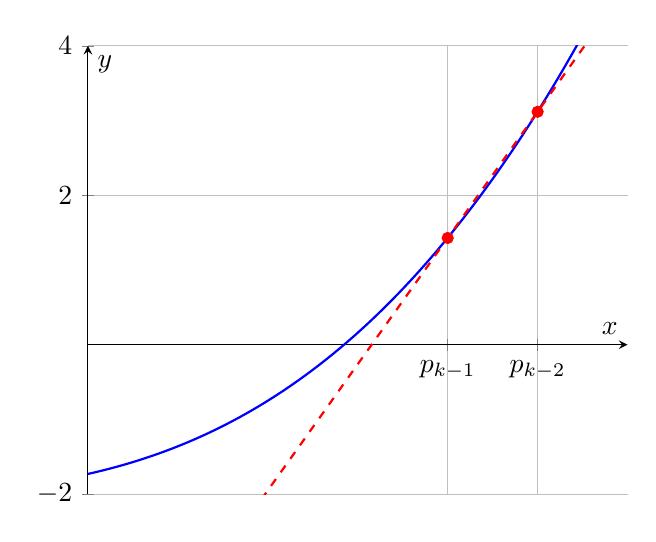
\begin{tikzpicture}
    \begin{axis}[
      axis lines = middle,
      xmin=0, xmax=6,
      ymin=-2, ymax=4,
      xlabel={$x$}, ylabel={$y$},
      samples=100,
      domain=0:6,
      grid=major,
      xtick={4,5}, 
      xticklabels={$p_{k-1}$, $p_{k-2}$}
      ]
            % Function plot
      \addplot[blue, thick] {0.01*(x+3)^3 - 2};

            % Compute function values
      \pgfmathsetmacro{\yA}{0.01*(4+3)^3 - 2}
      \pgfmathsetmacro{\yB}{0.01*(5+3)^3 - 2}

            % Plot points
      \addplot[red, only marks, mark=*] coordinates {(4, \yA)};
      \addplot[red, only marks, mark=*] coordinates {(5, \yB)};

            % Draw secant line
      \addplot[red, dashed, thick] 
        {(\yB - \yA) / (5 - 4) * (x - 4) + \yA};
      %
      %       % Equation label near midpoint
      % \node[anchor=south, red] at (axis cs: 4.5, (\yA+\yB)/2) 
      %   {\small $y = \frac{\yB - \yA}{5 - 4} (x - 4) + \yA$};

    \end{axis}
  \end{tikzpicture}
\end{center}

both newton's method and the secant method have the limitation that they may
diverge when the initial guess is not sufficiently close to the root. In 
bisection, we used the idea of bracketing the root at each step to ensure
convergence. 

\section{False Position}

If instead of considering a midpoint approximation for the root \newline
($\displaystyle p_k \approx p_0 + \frac{p_1 - p_0}{2}$), we consider a
secant approximation for the root (based on the endpoints of the interval).
This is called the \textbf{Method of False Position}.

\[
p_k \approx p_1 - f(p_1) \frac{p_1-p_0}{f(p_0)-f(p_1)}
.\]

\section{oops, skipped a bunch of pages}

\section{Error Analysis}

We want to be able to give a more precise description of how a method converges
to a the solution. For example, consider finding a root for the polynomial

\[
x^3 + 4x^2 - 10 = 0
.\]

with two different methods (A and B). Suppose that the errors produced by these 
methods are as given below.

\begin{table}[h]
    \centering
    \begin{tabular}{|c|c|c|}
        \hline
        & \textbf{Method A} & \textbf{Method B} \\
        \hline
        $|p - p_0|$ & 0.134769987 & 0.134769987 \\
        $|p - p_1|$ & 0.078276245 & 0.008103332 \\
        $|p - p_2|$ & 0.037310791 & 0.000003811 \\
        $|p - p_3|$ & 0.019771639 & 0.000000000 \\
        $|p - p_4|$ & 0.009940240 & \text{to all significant digits} \\
        \hline
    \end{tabular}
    \caption{Comparison of Methods A and B}
\end{table}

Notice that the error for method $A$ decreases by a constant factor (about 2)
at each iteration. For method $B$, the error drops off much more quickly. The
error at step $n$ is roughly proportional to the error at step $n-1$, squared.

\textbf{Both of these behaviours can be quantified.}

\noindent\defn Suppose $\{ p_n \}_{n=0}^\infty$ is a sequence that converges to $p$,
with $p_n \neq p$ for all $n$. If positive constants $\lambda$ and $\alpha$
exist with $\displaystyle \lim_{n\to\infty} \frac{|p_{n+1}-p|}{|p_n -p|^\alpha} = \lambda$
then $\{ p_n \}_{n=0}^\infty$ converges to $p$ of order $\alpha$, with asymptotic
error constant $\lambda$.

Notice that:
\begin{itemize}
\item a sequence with high order of convergence converges more rapidly than a
  sequence with a lower order.
\item the constant $\lambda$ affects the speed of convergence, but is not as
  important as the order ($\alpha$).
\item We want a large $\alpha$. $\alpha \geq 1$ is sufficient. \\
  If $\alpha = 0.5$, for example, then the error at $k$ is proportional
  to the square root of the error at $k-1$. This is not a good behaviour.
\end{itemize}

\subsection{Common Cases}

For different values of $\alpha$, we observe the following convergence behaviors:

\begin{itemize}
    \item $\alpha = 1$, $\lambda < 1$: Linearly convergent.
    \[ \bigEps_{n+1} \approx \lambda \bigEps_n \]
    
    \item $\alpha = 2$: Quadratically convergent.
    \[ \bigEps_{n+1} \approx \lambda \bigEps_n^2 \]
    
    \item $\alpha$ does not have to be an integer. For example, the secant method has:
    \[ \alpha = \frac{1+\sqrt{5}}{2} < 2. \]
\end{itemize}

\textbf{In order to truly understand the behaviour of a method, we need to
  find both the order and the asymptotic error constant.}

\section{Thm (2.7 of Text)}

Let $g\in C[a,b]$ s.t. $g(x) \in [a, b]$ for all $x \in [a, b]$.

Suppose, in addition, that $g'$ is continuous on $(a,b)$ and a constant
$0\leq k<1$ exists with $|g'(x)|\leq k$ for all $x\in (a,b)$.

If $g'(p) \neq 0$, then for any number $p_0$ in $[a,b]$ the sequence 

\[
  p_n = g(p_{n-1}) \text{ for } n\geq 1
.\]

converges only linearly to the unique fixed point $p$ in $[a,b]$.

\proof We know from the fixed point theorem that the sequence converges to $p$.
since $g'$ exists on $[a,b]$ we can apply the mean value theorem to g:

\[
\underbrace{g(p_n) - g(p)}_{p_{n+1} - p} = g'(\xi_n)(p_n - p)
.\]

where $\xi_n$ is between $p_n$ and $p$. Thus,

\[
  \frac{p_{n+1}-p}{p_n-p} = g'(\xi_n)
.\]

and fixed point iteration gives linear convergence with asymptotic error
constant $|g'(p)|$ whenever $g'(p) \neq 0$.


\section{Thm (2.7 of Text)}

Let $g\in C[a,b]$ s.t. $g(x) \in [a, b]$ for all $x \in [a, b]$.

Suppose, in addition, that $g'$ is continuous on $(a,b)$ and a constant
$0\leq k<1$ exists with $|g'(x)|\leq k$ for all $x\in (a,b)$.

If $g'(p) \neq 0$, then for any number $p_0$ in $[a,b]$ the sequence 

\[
  p_n = g(p_{n-1}) \text{ for } n\geq 1
.\]

converges only linearly to the unique fixed point $p$ in $[a,b]$.

\proof We know from the fixed point theorem that the sequence converges to $p$.
since $g'$ exists on $[a,b]$ we can apply the mean value theorem to g:

\[
\underbrace{g(p_n) - g(p)}_{p_{n+1} - p} = g'(\xi_n)(p_n - p)
.\]

where $\xi_n$ is between $p_n$ and $p$. Thus,

\[
  \frac{p_{n+1}-p}{p_n-p} = g'(\xi_n)
.\]

and fixed point iteration gives linear convergence with asymptotic error
constant $|g'(p)|$ whenever $g'(p) \neq 0$.

\proof...

Thus $\displaystyle \lim_{n\to\infty} \frac{|p_{n+1}-p|}{|p_n-p|} = |g'(p)|$
and fixed-point iteration gives linear convergence with asymptotic error 
constant $|g'(p)|$ whenever $g'(p) \neq 0$.

Method $A$ was the fixed-point iteration method defined by the iteration
function

\[
  g(x) = \frac{1}{2} (10-x^3)^{1/2}
.\]

Notice that:

\begin{align*}
g'(p=1.365230013)
&= -\frac{3}{4}x^2(10-x^3)^{-1/2} \\
&= -0.51 \neq 0
\end{align*}

so the theorem applies if we consider the interval $[1, 1.5]$ and we see that
linear convergence is obtained. On the other hand, Method $B$ was the fixed
point iteration method defined by the iteration function

\[
g(x) = x-\frac{x^3+4x^2-10}{3x^2+8x}
.\]

This method gave quadratic convergence, but the theorem cannot be applied 
because

\[
g'(p) = 0
.\]

We saw last day that higher order convergence for fixed point method can 
occur only when $g'(p) = 0$. It is possible under certain reasonable conditions
to obtain quadratic convergence...

\section{Theorem (2.8 of Text)}

Let $p$ be a solution of the equation $x = g(x)$.

Suppose $g'(p) = 0$ and $g''$ is continuous and strictly bounded by $M$ on an
open interval $I$ containing $p$. Then, there exists a $\delta > 0$ such that
for $p_0 \in [p-\delta, p+\delta]$, the sequence defined by $p_n = g(p_{n-1})$
when $n\geq 1$ converges at least quadratically to $p$.

Moreover, for sufficiently large values of $n$, 

\[
|p_{n+1} - p| < \frac{M}{2} |p_n - p|^2
.\]

\proof... (see lecture notes)

Thus the sequence $\{ p_n \}_{n=0}^\infty$ converges quadratically if
$g''(p) \neq 0$ and higher order convergent if $g''(p) = 0$. Also, we know
$|g''| < M $ so 

\[
|p_{n+1} - p| < \frac{M}{2} |p_n - p|^2
.\]

So the idea behind finding iteration methods with a high order of convergence
is to look for schemes whose derivatives are zero at the fixed point.

\section{Newton's Method}

\begin{align*}
  g(x) &= x-\frac{f(x)}{f'(x)} \\
  g'(x) &= 1-\frac{[f'(x)]^2 - f(x) f''(x)}{[f'(x)]^2} \\
        &= \frac{f(x)f''(x)}{[f'(x)]^2} \\
\end{align*}

$\therefore g'(p) = 0$ provided $f'(p) \neq 0$.

$\therefore$ Newton's Method satisfies the derivative condition for \thm 2.8.

\pagebreak

Let's take another look at Newton's Method. Consider using Newton's Method to
find the roots of

\[
p^3 - p^3 - p + 1 = 0
.\]

Newton's Method here is

\[
  p_{n+1} = p_n = \frac{p_n^3 - p_n^2 - p_n + 1}{3p_n^2 - 2p_n -1}
.\]

Starting from $p_0 = 1.1$ we find

\begin{table}[h]
  \centering
  \begin{tabular}{c|c}
    \textbf{Iteration} & \textbf{Value} \\
    \hline
    $p_0$ & 1.1 \\
    $p_1$ & 1.05116\ldots \\
    $p_2$ & 1.02589\ldots \\
    $p_3$ & 1.01303\ldots \\
    $p_4$ & 1.00653\ldots \\
    $p_5$ & 1.00327\ldots \\
    \vdots & \vdots
  \end{tabular}
  \caption{Numerical Iterations}
  \label{tab:iterations}
\end{table}

Which is very slow (Linear) convergence to the root (which is $p=1$).

Why is this?

In Newton's Method, we need to find $f'(p) \neq 0 $ to obtaine quadratic 
convergence. Notice that

\[
  f'(p) = 3p^2 - 2p - 1 |_{p=1} = 0
.\]

So the theorem doesn't hold. Moreover, factoring $f$:

\[
f(x) = (x-1)^2(x+1)
.\]

we see that $x=1$ is a zero with multiplicity of $2$.

\defn A solution $p$ of $f(x) = 0$ is a zero of multiplicity $m$ of $f$ if for 
$x\ne p$ we can write $f(x) = (x-p)^m q(x)$ where $\lim_{x\to p} q(x) \neq 0$.

Simple zeros are those that have multiplicity $1$.

Thus Newton's Method can only be applied to simple zeros of a function.
Identification fo the multiplicity of a zero is often made easier by the two
following theorems.

\thm 2.10

$f\in C'[a,b]$ has a simple zero at $p$ in $(a,b)$ if and only if $f(p) = 0$
but $f'(p) \neq 0$.

\thm 2.11

The function $f\in C^m[a,b]$ has a zero of multiplicity $m$ at $p$ if and only
if 

\[
  0 = f(p) = f'(p) = f''(p) = \dots = f^{(m-1)}(p)
.\]

but $f^{(m)}(p) \neq 0$.

We want to obtain quadratic convergence with Newton's Method for multiple roots.

One approach is to define a new function

\[
  \mu(x) = f\frac{(x)}{f'(x)}
.\]

We assume $p$ is a zero of multiplicity $m$ and $f(x) = (x-p)^m q(x)$ where
$q(p) \neq 0$. Then,

\begin{align*}
  \mu(x) &= \frac{(x-p)^m}{m(x-p)^{m-1} q(x) + q'(x)(x-p)^m} \\
  &= \frac{(x-p)q(x)}{mq(x) + q'(x) (x-p)}  \\
  &= (x-p) \frac{q(x)}{mq(x)+q'(x-p)} \\
  q(p) \neq 0 \quad\text{therefore, } &\mu(p) \text{ has a simple root at } x=p
\end{align*}

so $\mu(p) = 0$, but $\displaystyle \frac{q(p)}{mq(p) + q'(p)(p-p)} = \frac{1}{m} \neq 0$.
and $p$ is a zero of multiplicity $1$ of $\mu(x)$.

\textbf{Good:}
\begin{itemize}
  \item Quadratic convergence for all roots
\end{itemize}

\textbf{Bad:}
\begin{itemize}
  \item Need $f''$
  \item $\mu$ is more expensive to work with
  \item $\mu$ might give more roundoff error
\end{itemize}


% \section{Continued from Lecture 18}

Newton's Method can only be applied to simple zeros of a function.
Identification fo the multiplicity of a zero is often made easier by the two
following theorems.

\thm 2.10

$f\in C'[a,b]$ has a simple zero at $p$ in $(a,b)$ if and only if $f(p) = 0$
but $f'(p) \neq 0$.

\thm 2.11

The function $f\in C^m[a,b]$ has a zero of multiplicity $m$ at $p$ if and only
if 

\[
  0 = f(p) = f'(p) = f''(p) = \dots = f^{(m-1)}(p)
.\]

but $f^{(m)}(p) \neq 0$.

We want to obtain quadratic convergence with Newton's Method for multiple roots.

One approach is to define a new function

\[
  \mu(x) = f\frac{(x)}{f'(x)}
.\]

We assume $p$ is a zero of multiplicity $m$ and $f(x) = (x-p)^m q(x)$ where
$q(p) \neq 0$. Then,

\begin{align*}
  \mu(x) &= \frac{(x-p)^m}{m(x-p)^{m-1} q(x) + q'(x)(x-p)^m} \\
  &= \frac{(x-p)q(x)}{mq(x) + q'(x) (x-p)}  \\
  &= (x-p) \frac{q(x)}{mq(x)+q'(x-p)} \\
  q(p) \neq 0 \quad\text{therefore, } &\mu(p) \text{ has a simple root at } x=p
\end{align*}

so $\mu(p) = 0$, but $\displaystyle \frac{q(p)}{mq(p) + q'(p)(p-p)} = \frac{1}{m} \neq 0$.
and $p$ is a zero of multiplicity $1$ of $\mu(x)$.

\textbf{Good:}
\begin{itemize}
  \item Quadratic convergence for all roots
\end{itemize}

\textbf{Bad:}
\begin{itemize}
  \item Need $f''$
  \item $\mu$ is more expensive to work with
  \item $\mu$ might give more roundoff error
\end{itemize}

We return to finding the roots of

\[
p^3 - p^3 - p + 1 = 0
.\]

Apply:

\begin{table}[h]
    \centering
    \begin{tabular}{c c c}
        \toprule
         & Newton's Method & Modified Newton's Method \\
        \midrule
        $p_0$ & 1.1 & 1.1 \\
        $p_1$ & 1.05116... & 0.997735... \\
        $p_2$ & 1.02589... & 0.999999... \\
        $p_3$ & 1.01303... &  \\
        $p_4$ & 1.00653... &  \\
        $p_5$ & 1.00327... &  \\
        \bottomrule
    \end{tabular}
    % \caption{Comparison of Newton's Method and Modified Newton's Method}
    % \label{tab:newton_methods}
\end{table}

This table shows that Newton's Method has linear convergence, and the Modified
Newton's Method has quadratic convergence.

\section{Congervence Speed and Acceleration}

Suppose that we are given a linearly convergent sequence, and that we want to
speed up the convergence. We want to analyze the behaviour of the error and use
this knowledge to greatly reduce the error. 

For example, we saw last day that the iterator method with 

\begin{align*}
  p_{n+1} &= g(p_n) \\
  \text{and } g(x) &= \frac{1}{2}\sqrt{10-x^3}
\end{align*}

gives only linear convergence and the limit $p=1.3652$

\begin{table}[h]
    \centering
    \begin{tabular}{c c}
        \toprule
        Iteration & $p - p_n$ \\
        \midrule
        $p - p_0$ & $-0.13476\ldots$ \\
        $p - p_1$ & $+0.07827\ldots$ \\
        $p - p_2$ & $-0.03710\ldots$ \\
        $p - p_3$ & $+0.01977\ldots$ \\
        $p - p_4$ & $-0.00994\ldots$ \\
        \bottomrule
    \end{tabular}
    % \caption{Error progression in iterations}
    % \label{tab:error_progression}
\end{table}

Notice that the \uline{ratio} of the errors is fairly constant- we can use this
idea to accelerate the convergence of the method.

Suppose $\displaystyle \frac{p_{n+1}-p}{p_n-p} \approx \frac{p_{n+2}-p}{p_{n+1}-p}$

\[
  \therefore p \approx \frac{p_n p_{n+1} - p_{n+1}^2}{p_{n+2}-2p_{n+1}+p_n}
.\]

or,

\[
  p \approx p_n - \frac{p_{n+1}^2 - 2p_n p_{n+1} + p_n^2}{p_{n+2}-2p_{n+1}+p_n}
.\]

which is derived by adding and subtracting $p_n$ to the right hand side.

The corresponding sequence

\[
  \hat{p}_{n+1} = p_n - \left[ \frac{p_{n+1}^2-2p_np_{n+1}+p_n^2}{p_{n+2}-2p_{n+1}+p_n} \right]
.\]

is known as Aitken's Method.

\pagebreak
Applying Aitken's method to our previous sequence,

\begin{table}[h]
    \centering
    \begin{tabular}{c c | c c}
        \toprule
        \multicolumn{2}{c|}{Fixed Point Iteration} & \multicolumn{2}{c}{Aitken's Method} \\
        \midrule
        Iteration & $p - p_n$ & Iteration & $\hat{p} - p_n$ \\
        \midrule
        $p - p_0$ & $-0.13476\ldots$ & $\hat{p} - p_0$ & $0.00090088$ \\
        $p - p_1$ & $+0.07827\ldots$ & $\hat{p} - p_1$ & $0.00023088$ \\
        $p - p_2$ & $-0.03731\ldots$ & $\hat{p} - p_2$ & $0.00006107$ \\
        $p - p_3$ & $+0.01977\ldots$ & $\hat{p} - p_3$ & $0.00001592$ \\
        $p - p_4$ & $-0.00994\ldots$ & $\hat{p} - p_4$ & $0.00000418$ \\
        \bottomrule
    \end{tabular}
    % \caption{Error progression in Fixed Point Iteration and Aitken's Method}
    % \label{tab:fixed_aitken}
\end{table}

we notice that Aitken's Method is much faster.
It can be shown that the following theorem holds:

\section{Theorem (2.13 of Text)}

Suppose that $\{ p_n \}$ is a sequence that converges linearly to the limit $p$
and that for all sufficiently large values of $n$ we have $(p_n-p)(p_{n+1}-p) > 0$.

Then the sequence $\{ \hat{p}_{n=0}^\infty \}$ converges faster than $\{ p_n \}_{n=0}^\infty$.
to $p$ in the sense that $\displaystyle \lim_{n\to\infty} \frac{\hat{p}_n - p}{p_n-p} = 0$

The theorem does not apply to alternating sequences, but as we saw from our 
example it is often very useful even there for accelerating convergence.

Finally, we remark that this method is often written using difference operations 
to simplify the notation.

... sorry i missed a bunch here

\section{Zeros of Polynomials}

We want to compute the zeros (roots) of polynomials. A polynomial of degree $n$
has the form

\[
  P(x) = a_nx^n + a_{n-1}x^{n-1} + \dots + a_1x+a_0
.\]

where $a_i , i=0,\dots,n$ are constants and $a_n \neq 0$.

\subsection{Fundamental Theorem of Algebra}

If \( P \) is a polynomial of degree \( n \geq 1 \), then \( P(x) \) has at least one (possibly complex) root.

\subsubsection*{Corollary:}
If \( P(x) \) is a polynomial of degree \( n \geq 1 \), then there exist unique constants \( x_1, x_2, \dots, x_k \) (possibly complex), and positive integers \( m_1, m_2, \dots, m_k \) such that

\[
  \sum_{i=1}^{k} m_i = n
\]

and 

\[
  P(x) = a_n (x - x_1)^{m_1} (x - x_2)^{m_2} \dots (x - x_k)^{m_k}.
\]

\subsubsection*{Corollary:}
Let \( P \) and \( Q \) be polynomials of degree at most \( n \). If \( x_1, x_2, \dots, x_{n+1} \) with \( n+1 > n \) are distinct numbers with 

\[
  P(x_i) = Q(x_i) \quad \text{for } i = 1,2, \dots, n+1,
\]

then 

\[
  P(x) = Q(x) \quad \text{for all } x.
\]

We want to use Newton's Method to locate the approximate roots of $P$. It will
be necessary to evaluate $P$ and its derivative at specified values. We now 
direct our attention to efficient methods for this task. The idea is to use 
nesting to evaluate an arbitrary $n^{th}$ degree polynomial using only

\[
  n \text{ multiplications and } n \text{ additions}
.\]

For illustration, consider $n=4$. To evaluate 
$P(x) = a_4x^4 + a_3x^3 + a_2x^2 + a_1x+a_0$, we write:

\[
  P(x) = \left(\left(\left(\left(a_4x+a_3\right)x+a_2\right)x+a_1\right)x+a_0
.\]

Algorithmically,

\begin{enumerate}
  \item set $b_4 = a_4$
  \item set $b_3 = b_4x + a_3$
  \item set $b_2 = b_3x + a_2$
  \item set $b_1 = b_2x + a_1$
  \item set $b_0 = b_1x + a_0$
\end{enumerate}

Now $b_0$ gives the value $P(x)$.

For general polynomials of degree $n:$

\begin{align*}
  b_n &= a_n \\
  b_k &= a_k+b_{k+1}x \qquad\qquad 0 \leq k \leq n-1 \\
  \text{and } b_0 &= P(x) \\
\end{align*}

we also want $P'(x)$. Differentiate each of the steps listed above, keeping in
mind that $b_i$ is a function of $x$. We get:

\begin{align*}
  b_n ' &= 0 \\
  b_k' &= b_{k+1}'x + b_{k+1} \\
  \text{and } b_0' &= P'(x) \\
\end{align*}

Relabel: $c_{n+1} = b_n'$. Then an efficient method for computing $P'(x)$ is

\begin{align*}
  c_n &= a_n \\
  c_k &=  c_{k+1}x + b_{k} \\
  \text{and then } c_1 &= P'(x) \\
\end{align*}

This is called Horner's Method for evaluating a polynomial.

\section{Horner's Method}

Honer's Method has another useful property. 

Consider $P(x)$

\begin{align*}
    &= a_n x^n + a_{n-1} x^{n-1} + \dots + a_1 x + a_0 \\
    &= b_n x^n + (b_{n-1} - b_n x_0) x^{n-1} + \dots + (b_1 - b_2 x_0) x + (b_0 - b_1 x_0) \\
    &= (b_n x^{n-1} + b_{n-1} x^{n-2} + \dots + b_2 x + b_1) x \\
    &\qquad - (b_n x^{n-1} + b_{n-1} x^{n-2} + \dots + b_2 x + b_1) x_0 \\
    &\qquad + b_0 \\
    &= (b_n x^{n-1} + b_{n-1} x^{n-2} + \dots + b_2 x + b_1) (x - x_0) + b_0
\end{align*}

This property is useful because it gives us a way to find the next approximate
zero after we have found our first zeros.

\ie If $x_0$ is a root $P(x_0) = b_0 = 0\implies Q(x) (x-x_0) = P(x)$

so we can find the next root by examining roots of $Q(x)$.

Suppose we want additional roots of $P$. If $x_0$ is an approximate root of $P$,

\[
  P(x) \approx Q(x) (x-x_0) 
.\]

and the next step is toa pply Newton's Method to 

\[
  \displaystyle Q(X) = \frac{P(x)}{(x-x_0)}
.\]

this process is called deflation.


\section{Approximation and Interpolation}

It is often useful or necessary to approximate a complicated or expensive function,
or a function only known at a discrete set of points, by a smpler function
which can be computed or evaluated more easily over a whole interval. When the
function in question is known accurately at a discrete set of points, we are
inclined to use an interpolation procedure- where the graph of the approximating 
function runs exactly through the points of the discrete set. 

If the dataset is expected to contain error, which is the case for measurements
or observations in experimental studies, a better strategy is to allow the
graph of the approximating function to stray from the data points.

% insert image here

A useful and well known class of functions for mapping the set of real numbers
into itself is the class of algebraic polynomials.

\[
  P_n(x) = a_nx^n + a_{n-1}x^{n-1} + \dots + a_1x + a_0
.\]

where $n$ is a non-negative integer and $a_i$ are real constants. Polynomials 
have the desirable property that they can approximate \uline{any} function
over a closed, bounded interval.

This desired property is precisely captured by the \textbf{Weierstrass 
Approximation Theorem}

\pagebreak

\subsection{The Weierstrass Approximation Theorem}

Suppose $f \in C[a,b]$. 

$\forall \bigEps > 0 \exists P \in \{ \mathbb{P}_n , C[a,b] \}$ such that

\[
  |f(x)-P(x)| < \epsilon \forall x \in [a,b]
.\]

\begin{figure}[h]
    \centering
    \resizebox{0.8\textwidth}{!}{%
        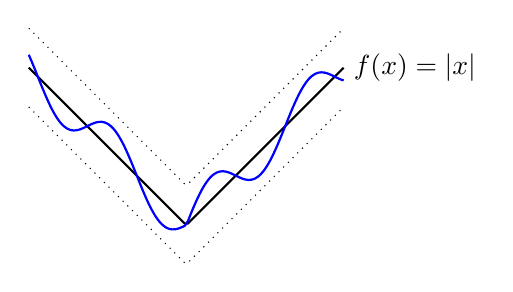
\begin{tikzpicture}
            % Define the function
            \draw[thick] plot[samples=100,domain=-2:2] (\x,{abs(\x)}) node[right] {$f(x) = |x|$};

            % Epsilon bounds
            \draw[dotted] plot[samples=100,domain=-2:2] (\x,{abs(\x) + 0.5});
            \draw[dotted] plot[samples=100,domain=-2:2] (\x,{abs(\x) - 0.5});

            % Labeling epsilon
            % \draw[->] (1,1.5) -- (1.1,1.2) node[midway,right] {$\varepsilon$};
            % \draw[->] (-1,1.5) -- (-1.1,1.2) node[midway,left] {$\varepsilon$};

            % Approximation function (squiggly)
            \draw[thick,blue] plot[smooth, samples=100, domain=-2:2] (\x, {0.3*sin(5*\x r) + abs(\x)});

        \end{tikzpicture}%
    }
    \caption{Polynomial approximation to $f(x) = |x|$.}
\end{figure}

This is a very strong theorem, as it only requires $f(x)$ to be continuous on 
the interval, and not necessarily differentiable.

Unfortunately, the Weierstrass Approximation Theorem does not tell us how to 
select such a polynomial. Many would immediately jump to using Taylor series
polynomials for polynomial interpolation, however, Taylor series' concentrate
their accuracy at the point $a$ rather than over the entire interval, and are
typically poorly suited for interpolation.

\subsubsection{Taylor Series Polynomials}

\[
P_n(x) = f(a) + f'(a)(x-a) + \frac{f''(a)}{2!}(x-a)^2 + \dots + \frac{f^{(n)}(a)}{n!}(x-a)^n
.\]

A particularly clear demonstration of this drawback is seen for

\[
f(x) = \frac{1}{x} \qquad \text{expanded about } x_0 = 1
.\]

Then,

\begin{align*}
  P_n(x) &= \sum_{k=0}^n \frac{f^{(k)}(1)}{k!}(x-1)^k\\
         &= \sum_{k=0}^n (-1)^k(x-1)^k \\
\end{align*}

To approximate $f(3)=\frac{1}{3}$ by $P_n(3)$ for increasing values of $n$, we
see a dramatic and catastrophic failure: 

\begin{table}[h]
    \centering
    \renewcommand{\arraystretch}{1.4}
    \begin{tabular}{|c|c|c|c|c|c|c|c|c|}
        \hline
        \( n \) & 0 & 1 & 2 & 3 & 4 & 5 & 6 & 7 \\ 
        \hline
        \( P_n(3) \) & 1 & -1 & 3 & -5 & 11 & -21 & 43 & -85 \\ 
        \hline
    \end{tabular}
    \caption{Values of \( P_n(3) \) for increasing \( n \).}
\end{table}

We will insetad focus on methods which use information throughout the entire 
interval to approximate $f$.

\section{Polynomial Interpolation}

We now assume that the given dataset is exact and represents values of some
unknown function. We want to find the polynomial $P_n(x)$ of the smallest 
possible degree $n$ such that

\[
P_n(x_k) = f_k \qquad k = 1,2, \dots, N
.\]

for $N+1$ distinct interpolation points $x_0,\dots,x_N$ and $N+1$ values 
$\underbrace{f_0,\dots,f_N}_{\text{data points}}$.

To solve this problem, we will first investigate the simpler problem where all
the data equals zero, except at one point.

We are looking for a polynomial $L_m(x)$ of degree $\leq N$ such that

\[
  L_m(x_k) = \delta_{mk} \qquad = \begin{cases}
    1 & k = m \\
    0 & k \neq m
    \end{cases}
.\]


\begin{center}

\begin{tikzpicture}[overlay, remember picture]
    \draw[thick,->] (0,0) node[below]{\textbf{Kronecker Delta}} to (-1.1,0.8);
\end{tikzpicture}
\end{center}

This is easy to find. Since the polynomial must vanish at the points 
$x_k, k\neq m$, it must contain the factors

\[
  (x-x_k) \qquad \text{for } k \neq m
.\]

\[
\therefore L_m(x) = c \cdot \prod_{k=0; k\neq m}^N(x-x_k)
.\]

The constant is determined by the condition $L_m(x_m) = 1$.

\[
\implies L_m(x) = \prod_{k=0; k\neq m}^{N}  \frac{x-x_k}{x_m-x_k}
.\]

Typically, 
\begin{center}
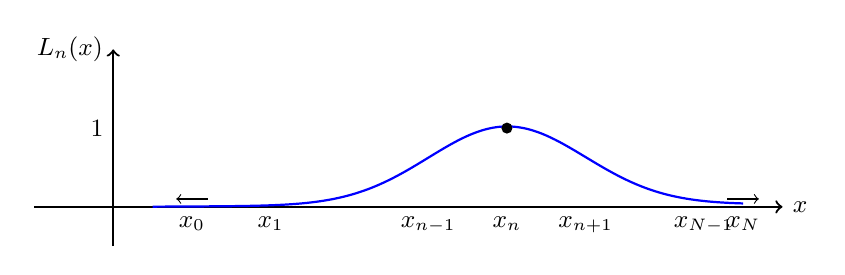
\begin{tikzpicture}
    % Axes
    \draw[thick,->] (-1,0) -- (8.5,0) node[right] {\small $x$}; % x-axis
    \draw[thick,->] (0,-0.5) -- (0,2) node[left] {\small $L_n(x)$}; % y-axis

    % Labels on axes
    \node[left] at (0,1) {\small 1}; % Label at y = 1

    % Points on x-axis
    \foreach \x/\label in {1/$x_0$, 2/$x_1$, 4/$x_{n-1}$, 5/$x_n$, 6/$x_{n+1}$, 7.5/$x_{N-1}$, 8/$x_N$}
        \node[below] at (\x,0) {\small \label};

    % Sinusoidal-like Lagrange basis function
    \draw[thick,blue,domain=0.5:8,samples=100,smooth] 
        plot (\x, {exp(-0.5*(\x-5)^2) * cos(2*pi*(\x-5)/3) + 0.05*sin(5*\x)});

    % Highlight peak at x_n
    \fill (5,1) circle (2pt);
    
    % Small arrows at edges
    \draw[->] (7.8,0.1) -- (8.2,0.1);
    \draw[->] (1.2,0.1) -- (0.8,0.1);
    
\end{tikzpicture}
\end{center}

These polynomials are the building blocks for deriving a polynomial
interpolating a general function. It is easy to see that

\[
  P(x) = \sum_{m=0}^N f_m < L_m(x)
.\]

is a polynomial of degree $\leq N$ satisfying the interpolation conditions.

This polynomial is called the $n^{th}$ \textbf{Lagrange Interpolating Polynomial} 

Recall that we wanted to find the polynomial $P_n(x)$ of smallest degree such
that 

\[
  P_n(x_k) = f_k \qquad k = 0,\dots,N
.\]

\subsection{Uniqueness}

Is this polynomial unique?

\textbf{Yes.} 

\proof Assume there are two different polynomials $p$ and $q$ of degree $\leq N$
which both satisfy the interpolation conditions. Their difference, $d=p-q$, is
also a polynomial of degree $\leq N$ and vanishes at the $N+1$ distinct points 
$x_0,\dots,x_N$.

However, a nonzero polynomial of degree $\leq N$ has at most $N$ zeros, this

\[
d = p-q = 0 \implies \begin{cases}
  p=q\\
  \text{ uniqueness}
\end{cases}
\]

$\therefore$ the $n^{th}$ Lagrange Interpolating Polynomial is the unique
interpolating polynomial satisfying the interpolation conditions.

\subsection{Example}

Fit a cubic through the first four points of the table 

\begin{table}[h]
    \centering
    \begin{tabular}{c|c|c}
        $i$ & $x^i$ & $f(x_i)$ \\
        \hline
        0 & 3.2 & 22.0 \\
        1 & 2.7 & 17.8 \\
        2 & 1.0 & 14.2 \\
        3 & 4.8 & 38.3 \\
        4 & 5.6 & 51.7 \\
    \end{tabular}
    % \caption{Tabular representation of given data}
    % \label{tab:data}
\end{table}

and use it to find the interpolated value for $x=3.0$.

\soln The $3^{rd}$ Lagrange Interpolating Polynomial is given by

\begin{align*}
    P(x) = &\ \frac{(x - x_1)(x - x_2)(x - x_3)}{(x_0 - x_1)(x_0 - x_2)(x_0 - x_3)} f_0 \\
    &+ \frac{(x - x_0)(x - x_2)(x - x_3)}{(x_1 - x_0)(x_1 - x_2)(x_1 - x_3)} f_1 \\
    &+ \frac{(x - x_0)(x - x_1)(x - x_3)}{(x_2 - x_0)(x_2 - x_1)(x_2 - x_3)} f_2 \\
    &+ \frac{(x - x_0)(x - x_1)(x - x_2)}{(x_3 - x_0)(x_3 - x_1)(x_3 - x_2)} f_3
\end{align*}

Substituting the values from the table and evaluating at $x=3.0$ gives 

\begin{align*}
    P(3.0) = &\ \frac{(3.0 - 2.7)(3.0 - 1.0)(3.0 - 4.8)}{(3.2 - 2.7)(3.2 - 1.0)(3.2 - 4.8)} (22.0) \\
    &+ \frac{(3.0 - 3.2)(3.0 - 1.0)(3.0 - 4.8)}{(2.7 - 3.2)(2.7 - 1.0)(2.7 - 4.8)} (17.8) \\
    &+ \frac{(3.0 - 3.2)(3.0 - 2.7)(3.0 - 4.8)}{(1.0 - 3.2)(1.0 - 2.7)(1.0 - 4.8)} (14.2) \\
    &+ \frac{(3.0 - 3.2)(3.0 - 2.7)(3.0 - 1.0)}{(4.8 - 3.2)(4.8 - 2.7)(4.8 - 1.0)} (38.3) \\
    &= 20.21
\end{align*}

Our next task is to develop estimates for the error. As it turns out, the form
of the error (but not necessarily the magnitude) resembles that of the $n^{th}$
Taylor Polynomial.

\subsection{Error Estimates}

*The lecture ended just before this section*

\thm (3.3 of Text)

Suppose $x_0, \dots, x_n$ are distinct numbers in the interval $[a,b]$ and
$f\in C^{n+1}[a,b]$. Then for each $x\in [a,b]$, a number $\xi(x)\in(a,b)$
exists with the property

\[
  f(x) = P(x) + \frac{f^{(n+1)}(\xi(x))}{(n+1)!} (x-x_0) (x-x_1) \dots (x-x_n)
.\]

\begin{center}

\begin{tikzpicture}[overlay, remember picture]
    \draw[thick,->] (-2,0) node[below]{\textbf{n-th Langrange Interpolating Polynomial}} to (-3.2,0.6);
\end{tikzpicture}
\end{center}

*do you guys like my diagrams with arrows?*


\section{Continued from Lecture 20}

Our next task is to develop estimates for the error. As it turns out, the form
of the error (but not necessarily the magnitude) resembles that of the $n^{th}$
Taylor Polynomial.

\subsection{Error Estimates}

\thm (3.3 of Text)

Suppose $x_0, \dots, x_n$ are distinct numbers in the interval $[a,b]$ and
$f\in C^{n+1}[a,b]$. Then for each $x\in [a,b]$, a number $\xi(x)\in(a,b)$
exists with the property

\[
  f(x) = P(x) + \frac{f^{(n+1)}(\xi(x))}{(n+1)!} (x-x_0) (x-x_1) \dots (x-x_n)
.\]

\begin{center}

\begin{tikzpicture}[overlay, remember picture]
    \draw[thick,->] (-2,0) node[below]{\textbf{n-th Langrange Interpolating Polynomial}} to (-3.2,0.6);
\end{tikzpicture}
\end{center}

Recall: If $f$ has $(n+1)$ continuous derivatives on $[a,b]$ and $P(x)$ is the 
interpolating polynomial of degree $\leq n$ for $f$ at the points 
$x_0, \dots, x_n$, then,

\[
  f(x) - P(x) = \frac{f^{(n+1)}(\xi (x))}{(n+1)!} \prod_{k=0}^{n} (x-x_k)
.\]

\Ex suppose you need to construct six-decimal-place tables for the common, or
base-10, logarithm function from $x=1$ to $x=10$ in a way that linear 
interpolation is accurate within $10^{-6}$ of the true value. Determine a bound
for the step size for this table.

Based on the following data:

\begin{table}[h]
    \centering
    \begin{tabular}{c c c}
        \toprule
        $i$ & $x_i$ & $f(x_i)$ \\
        \midrule
        0 & 3.2 & 22.0 \\
        1 & 2.7 & 17.8 \\
        2 & 1.0 & 14.2 \\
        3 & 4.8 & 38.3 \\
        4 & 5.6 & 51.7 \\
        \bottomrule
    \end{tabular}
    % \caption{Tabulated data of $x_i$ and $f(x_i)$ values}
    % \label{tab:data}
\end{table}

find approximations to $f(3)$ using the $2^{nd}$ and $3^{rd}$ Lagrange
interpolating polynomials.

\soln we will use $x_0, x_1$ and $x_3$ to build the $2^{nd}$ Lagrange
interpreting polynomial.

\begin{align*}
P_2(3) &= \frac{(3 - 2.7)(3 - 4.8)}{(3.2 - 2.7)(3.2 - 4.8)} (22.0) \\
&\quad + \frac{(3 - 3.2)(3 - 4.8)}{(2.7 - 3.2)(2.7 - 4.8)} (17.8) \\
&\quad + \frac{(3 - 3.2)(3 - 2.7)}{(4.8 - 3.2)(4.8 - 2.7)} (38.3) \\
&\approx 20.27
\end{align*}

We will use $x_0, x_1, x_2, x_3$ to build the $3^{rd}$ Lagrange
interpolating polynomial.

\begin{align*}
P_3(3) &= \frac{(3.0 - 2.7)(3.0 - 1.0)(3.0 - 4.8)}{(3.2 - 2.7)(3.2 - 1.0)(3.2 - 4.8)} (22.0) \\
&\quad + \frac{(3.0 - 3.2)(3.0 - 1.0)(3.0 - 4.8)}{(2.7 - 3.2)(2.7 - 1.0)(2.7 - 4.8)} (17.8) \\
&\quad + \frac{(3.0 - 3.2)(3.0 - 2.7)(3.0 - 4.8)}{(1.0 - 3.2)(1.0 - 2.7)(1.0 - 4.8)} (14.2) \\
&\quad + \frac{(3.0 - 3.2)(3.0 - 2.7)(3.0 - 1.0)}{(4.8 - 3.2)(4.8 - 2.7)(4.8 - 1.0)} (38.3) \\
&\approx 20.21
\end{align*}

Notice that:

\begin{enumerate}
\item We do not know the derivative values of $f$, therefore we cannot apply 
  the error formula. However, we can make an estimate for the error by examining
  polynomials of different degrees by using different nodes.

\item The $P_2$-calculation was not used to reduce the work in calculating $P_3$.
  We want to find a way to use previous degrees of $P$, especially since the 
  previous point implies that we will examine the results for Lagrange 
  polynomials of varying degrees.
\end{enumerate}

\noindent
We want to examine polynomials based on different nodes. In the last example, 
we considered the polynomial based on the nodes $x_0, x_1 \text{ and } x_3$

We will call this polyomial $\mathbf{P_{013}(x)}$

\noindent
We also considered the polynomial based on the nodes $x_0, x_1, x_2, x_3$

We will call this polyomial $\mathbf{P_{0123}(x)}$

Similarly, we make the following definition:

Let $f$ be a function defined at $x_0, x_1, x_2, \dots, x_n$ and suppose that
$m_1, m_2, \dots ,m_k$ are $k$ distinct integers with $0\leq m_i \leq n$ and
for each $i$. 

The Lagrange Interpolating Polynomial that agrees with $f$ at 
$x_m, x_{m2}, \dots, x_{mk}$ is denoted

\[
  P_{m_1, m_2, \dots, m_k}
.\]

Using this notation,

\[
P_0(x) = f(x_0)
\]

\[
P_1(x) = \frac{(x - x_1) f(x_0) + (x - x_0) f(x_1)}{x_0 - x_1}
\]

and 


\begin{align*}
  P_{0,1}(x) &= \left( \frac{x - x_1}{x_0 - x_1} \right) f(x_0) + \left( \frac{x - x_0}{x_1 - x_0} \right) f(x_1) \\
             &= \frac{(x - x_1) P_0(x) - (x - x_0) P_1(x)}{x_0 - x_1}
\end{align*}

So $P_{0,1}(x)$ can be recursively defined in terms of $P_0(x)$ and $P_1(x)$.

More generally:

\thm Let $f$ be defined at $x_0, x_1, \dots, x_k$ and $x_j$ and $x_i$ be two
distinct numbers in this set. Then

\[
  P_{0,1,\dots,k}(x) = 
  \frac{(x - x_j) P_{0,1,\dots,j,j+1,\dots,n}(x) - (x - x_i) P_{0,1,\dots,i-1,i+1,\dots,n}(x)}{x_i - x_j}
.\]

\proof I left out the proof.

The corresponding procedure is called Neville's Method. Here, values for each 
interpolating polynomial are generated using previous calculations.

\Ex $\displaystyle P_{0,1}(x) = \frac{(x-x_1)P_0 - (x-x_0) P_1}{(x_0 - x_1)}$ is
derived from $P_0 + P_1$. Correspondingly, $P_{1,2}(x)$ is derived from $P_1$
and $P_2$.

Written as a table:

\begin{figure}[h]
    \centering
    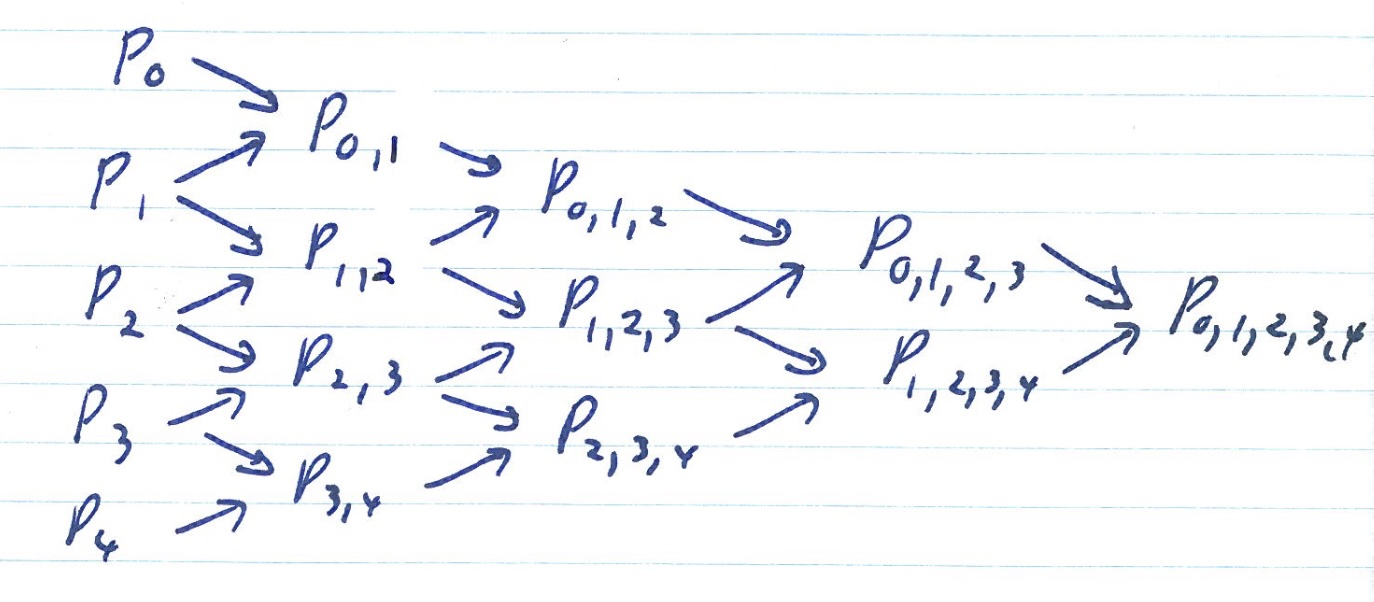
\includegraphics[width=0.8\textwidth]{./assets/Lecture 021 Neville's Method Table.jpg}
\end{figure}

\Ex suppose $x_j = j$ for $j=0,1,2,3$ and it is known that 

\begin{align*}
  &P_{0,1}(x) = 2x+1 \\
  &P_{0,2}(x) = x+1 \\
  &P_{1,2,3}(2.5) = 3
\end{align*}

Find $P_{0123}(2.5)$.

We have $P_{123}$ and we need another quadratic to find our $P_{0123}$

\[
P_{0,1,2} = \frac{(x-x_1)P_{02} (x) - (x-x_2) P_{01}(x)}{x_2 - x_1}
.\]

We evaluate $P_{02}(2.5) = 2.25$ and $P_{01}(2.5) = 6$

We have $x_1 = 1, x_2 = 2, x=2.5$

\[
  P_{012}(2.5) = 2.25 
.\]

\[
  P_{0123}(2.5) = \frac{(2.25-x_0)P_{123}(2.25) - (2.25-x_3)P_{012}(2.25)}{x_3 -
  x_0} = 2.875
\]


\section{Review}

\subsection{Polynomial Interpolation}
We have data for a function $f$ aat $x_0, x_1, \dots, x_n$

\subsection{Lagrange Interpolation}
\[
  \sum_{j=0}^n f(x_j) \underbrace{L_j(x)}_{0 \text{ at } x_i \text{ when } i \neq j}
.\]

Reminder: a degree $n$ polynomial interpolant for $n+1$ points is unique. This
means any polynomial interpolation method will give the same polynomial, just in
a different form.

\subsection{Divided Differences}

Divided differences is an easy way to add data points.

Assume we know $f(x)$ at several values for $x$.

% \begin{table}[h]
%   \centering
%   \begin{tabular}{cccc}
%     f_0 & f_1 & f_2 & f_3 \\
%     \hline
%     x_0 & x_1 & x_2 & x_3
%   \end{tabular}
% \end{table}

The $x_i$ points do \uline{not} need to be evenly spaced, or in any particular order.

We choose to represent our degree $n$ interpolating polynomial as follows:

\[
  P_n(x) = a_0 + a_1 (x-x_0) + a_2 (x-x_0) (x-x_1) + \dots + a_n (x-x_0) \dots (x-x_{n-1})
.\]

For every term we add, we interpolate another data point. We choose $a_i$ such
that $P_n(x) = f(x)$ at the points $x_0, x_1, \dots, x_n$.

The coefficients $a_i$ are determined by divided differences

\[
P_n (x_0) = f(x_0)
.\]

\[
  a_0 = f(x_0) = f[x_0]
.\]

Define the zero$^{th}$ divided difference

\[
  f[x_j] = f(x_j)
.\]

\[
a_0 + a_1(x_1-x_0) = f(x_1)
.\]

\[
  f[x_0] + a_1 (x_1-x_0) = f[x_1]
.\]

\[
a_1 = \frac{f[x_1] - f[x_0]}{x_1-x_0}
.\]

Define first divided difference

\[
  f[x_i, x_{i+1}] = f[x_{i+1}, x_i] = \frac{f[x_{i+1}]-f[x_i]}{x_{i+1}-x_i}
.\]

\[
  a_0 = f[x_0]
.\]

\[
  a_1 = f[x_0, x_1]
.\]

\[
  a_2 = f[x_0, x_1, x_2]
.\]

Define the second divided difference

\begin{align*}
  &f[x_i, x_{i+1}, x_{i+2}] \\
  &= \frac{f[x_{i+1}, x_{i+2}] - f[x_i, x_{i+1}]}{x_{i+2}-x_i} \\
\end{align*}

Define the $k^{th}$ divided difference for $x_i, \dots, x_{i+k}$

\begin{align*}
  &f[x_i, x_{i+1}, \dots, x_{i+k}] \\
  &= \frac{f[x_{i+1}, \dots, x_{i+k}] - f[x_i, \dots, x_{i+k-1}]}{x_{i+k}-x_i} 
\end{align*}

\[
  a_k = f[x_0, x_1, \dots, x_k]
.\]

This is Newton's interpolating divided difference formula.


\begin{align*}
  P(x) &= f[x_0] + f_[x_0, x_1] (x-x_0) \\
       &+ f[x_0, x_1, x_2] (x-x_0) (x-x_1) \\
       &+ \dots \\
       &+ f[x_0, x_1, \dots, x_n](x-x_0) \dots (x-x_{n-1})
\end{align*}

To compute an extra datapoint, we only need to compute one more term:

\[
  P_n(x) = P_{n-1}(x) + f[x_0, x_1, \dots, x_n](x-x_0) \dots (x-x_{n-1})
.\]

Note that while using this method, we do NOT need to have our $x_i$ points in
any particular order.

\subsubsection{Example}

\[
  (x_0, \dots, x_4) = (0.3, 1.0, 0.7, 0.6, 1.9)
.\]

Note that our points are not in order, or evenly spaced.

We are going to interpolate 

\[
  f(x) = 2x^3 - x^2 +x - 1
.\]

We can use a table!

Divided differences table:

% \begin{table}[h]
%   \centering
%   \begin{tabular}{c|c|c}
%     \( x_i \) & \( f[x_i] \) & f[x_i, x_{i+1}] \\
%     \hline
%     \( 0.3 \) & \( -0.736 \) & 2.48\\
%     \( 1.0 \) & \( 1.0 \) & 3.68\\
%     \( 0.7 \) & \( -0.104 \) & 2.24\\
%     \( 0.6 \) & \( -0.328 \) & 8.72\\
%     \( 1.9 \) & \( 11.008 \)
%   \end{tabular}
% \end{table}

\begin{center}
    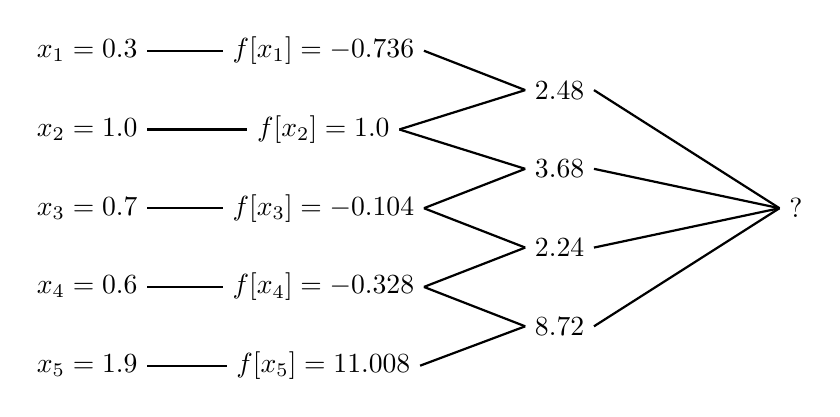
\begin{tikzpicture}
        % Nodes (x_i values)
        \node (X1) at (0, 4) {\( x_1 = 0.3 \)};
        \node (X2) at (0, 3) {\( x_2 = 1.0 \)};
        \node (X3) at (0, 2) {\( x_3 = 0.7 \)};
        \node (X4) at (0, 1) {\( x_4 = 0.6 \)};
        \node (X5) at (0, 0) {\( x_5 = 1.9 \)};

        % Nodes (f[x_i] values)
        \node (F1) at (3, 4) {\( f[x_1] = -0.736 \)};
        \node (F2) at (3, 3) {\( f[x_2] = 1.0 \)};
        \node (F3) at (3, 2) {\( f[x_3] = -0.104 \)};
        \node (F4) at (3, 1) {\( f[x_4] = -0.328 \)};
        \node (F5) at (3, 0) {\( f[x_5] = 11.008 \)};

        % Nodes (Third Column)
        \node (C1) at (6, 3.5) {\( 2.48 \)};
        \node (C2) at (6, 2.5) {\( 3.68 \)};
        \node (C3) at (6, 1.5) {\( 2.24 \)};
        \node (C4) at (6, 0.5) {\( 8.72 \)};

        % Final Result Node
        \node (Final) at (9, 2) {\( ? \)};

        % Connecting Lines (Tree Structure)
        \draw[thick] (X1.east) -- (F1.west);
        \draw[thick] (X2.east) -- (F2.west);
        \draw[thick] (X3.east) -- (F3.west);
        \draw[thick] (X4.east) -- (F4.west);
        \draw[thick] (X5.east) -- (F5.west);

        \draw[thick] (F1.east) -- (C1.west);
        \draw[thick] (F2.east) -- (C1.west);
        \draw[thick] (F3.east) -- (C2.west);
        \draw[thick] (F4.east) -- (C3.west);
        \draw[thick] (F5.east) -- (C4.west);

        \draw[thick] (F2.east) -- (C2.west);
        \draw[thick] (F3.east) -- (C3.west);
        \draw[thick] (F4.east) -- (C4.west);


        \draw[thick] (C1.east) -- (Final.west);
        \draw[thick] (C2.east) -- (Final.west);
        \draw[thick] (C3.east) -- (Final.west);
        \draw[thick] (C4.east) -- (Final.west);

    \end{tikzpicture}
\end{center}

The first entry in each column gives the coefficients

\begin{align*}
    P_4(x) &= -0.736 \\
           &\quad + 2.48(x-0.3) \\
           &\quad + 3(x-0.3)(x-1.0) \\
           &\quad + 2(x-0.3)(x-1.0)(x-0.7) \\
           &\quad + 0(x-0.3)(x-1.0)(x-0.7)(x-0.6) \\
           &\quad + 0(x-0.3)(x-1.0)(x-0.7)(x-0.6)(x-1.9).
\end{align*}

\section{KEY TAKEAWAY}

Basically, using the table, we can get all the constants we need to compute the
next datapoint by just looking back and grabbing the appropriate column.

\section{Midterm Review}

Find the rate of convergence as $h\to 0$:

\[
  \lim_{h \to 0} (e^h + e^{-h}) = 2
.\]

1. expand $e^h + e^{-h} - 2$ using taylor series

\[
  e^h = 1+h + \frac{h^2}{2!} + \frac{h^3}{3!} + O(h^4)
.\]


\begin{align*}
  e^h + e^{-h} -2 &= \left(1+h + \frac{h^2}{2!} + \frac{h^3}{3!} + O(h^4) \right ) \\
                  &\quad + \left ( 1-h+\frac{h^2}{2!}-\frac{h^3}{3!}+O(h^4) \right ) \\
                  &-2 \\
                  &= h^2 + O(h^3) = O(h^2)
\end{align*}

For midterm, know:
\begin{itemize}
  \item common taylor series 
    % ($e^x, \sin(x), \cos(x), \ln(1+x), (1+x)^{-p}$) 
  \item Partial Pivoting w/ or w/0 scaling
\end{itemize}

\subsection{Another Problem}

Consider

\begin{align*}
  x_1 + 30x_2 &= 50 \\
  5x_1 - 10x_2 &=  3
\end{align*}

Use Gaussian Elimination w/ scaled partial pivoting to take the system to upper
triangular form.

$\displaystyle \frac{1}{30} < \frac{5}{10} \implies$ we need to exchange rows

\begin{align*}
  5x_1 - 10x_2 &=  3 \\
   x_1 + 30x_2 &= 50 \\
  \hline
  5x_1 - 10x_2 &=  3 \\
  32x_2 = 50 - \frac{3}{5}
\end{align*}


\section*{Lecture Review}

In this lecture, he begins with a review of somet things that we covered in
lecture 22 and 21, which he was absent for and had a TA teach for him.

\subsection{Divided Differences}

Assume that $f(x)$ is known at several points along the x-axis. We do not assume
that the $x$'s are evenly spaced or even that the values are arranged in any
particular order.

We write the (any arbitrary) $n^{th}$ degree polynomial in the following way:

\[
  P_n(x) = a_0 + a_1 (x-x_0) + a_2 (x-x_0) (x-x_1) + \dots + a_n (x-x_0) \dots (x-x_{n-1})
.\]

\defn $P_n(x)$ is an interpolating polynomial for $f(x)$ at $x_0, x_1, \dots, x_n$
if we choose $a_i$ such that $P_n(x) = f(x))$ at the $n+1$ known points.

We want to find our $a_i$ to make $P_n(x)$ an interpolating polynomial, and we
can determine our $a_I$ by using what are called the \enquote{divided
differences.}

\subsubsection{The Zeroth Divided Difference}

First, we determine $a_0: P_n(x_0) = f(x_0) = a_0$, and define the
$\text{zero}^{\text{th}}$ (degree) divided difference as

\[
  f[x_i] = f(x_i)
,\]

\noindent
which is just the value of $f$ at $x_i$.

\subsubsection{The First Divided Difference}

Now we need to determine $a_1$:

\[
P_n(x_1) = f(x_1) = a_0 + (x_1 - x_0) a_1
.\]

Rearranging, we get

\[
a_i = \frac{f(x_1) - f(x_0)}{x_1 - x_0} = \frac{f[x_1] - f[x_0]}{x_1 - x_0}
.\]

which allows us to determine $a_1$ by using the $\text{zero}^{\text{th}}$ 
divided difference. We define the first divided difference of $f$ with respect
to $x_i$ and $x_{i+1}$ as

\[
  f[x_i, x_{i+1}] = f[x_{i+1}, x_i] = \frac{f[x_{i+1}]-f[x_i]}{x_{i+1}-x_i}
.\]


\subsubsection{The Second Divided Difference}

Similarly, the second divided difference is defined as 

\[
  f[x_i, x_{i+1}, x_{i+2}] = \frac{f[x_{i+1}, x_{i+2}] - f[x_i, x_{i+1}]}{x_{i+2}-x_i}
.\]

\subsubsection{The Kth Divided Difference}

In a similar fashion to the evaluation of $a_0$ and $a_1$, we can show

\[
  a_k = f[x_0, x_1, \dots, x_k]
.\]

This gives Newton's Interpolatory divided difference formula

\begin{align*}  
  P_n(x) &= f[x_0] + f[x_0, x_1] (x-x_0) \\
         &\quad+ f[x_0, x_1, x_2] (x-x_0) (x-x_1) \\
         &\quad+ \dots \\
         &\quad+ f[x_0, x_1, \dots, x_n](x-x_0) \dots (x-x_{n-1})
\end{align*}

\subsubsection{Disadvantages of Divided Differences}

\begin{itemize}
\item $P_n(x)$ could be expensive to evaluate
\item $P_n(x)$ does go through the datapoints, but between each datapoint, we
  could have large oscillations, which we expect as the generic behaviour of
  large degree polynomials.
  \subitem This is especially true near endpoints, where our datapoints are
  sparse and sections where our function is not smooth.
\end{itemize}

\section{Better Interpolating Polynomials - Ch2. Pt3. (14.1)}

The Lagrange Polynomial can oscillate wildly, except where contained between
datapoints that are in close proximity. We want our interpolating polynomial to
have the same \enquote{shape} as the function at the datapoints. In other words,
we want the tangent lines (first derivative) and the function itself to agree at
$(x_i, f_1)$

\subsection{Proof from (14.2).} 

This section is directly copied from the Chapter 3 Part 2 pdf.

\thm
If \( f \in C^1[a,b] \) and \( x_0, \ldots, x_n \in [a,b] \) are distinct, the interpolating polynomial of least degree agreeing with \( f \) at \( x_0, \ldots, x_n \) is the Hermite polynomial of degree at most \( 2n+1 \) given by

\[
H(x) = \sum_{j=0}^{n} f(x_j) H_j(x) + \sum_{j=0}^{n} f'(x_j) \hat{H}_j(x)
\]

where

\[
H_j(x) = \left[1 - 2(x - x_j)L_j'(x_j)\right] L_j^2(x)
\]

and

\[
\hat{H}_j(x) = (x - x_j) L_j^2(x)
\]

where \( L_j(x) \) denotes the Lagrange coefficient polynomial of degree \( n \).

\begin{proof}
See text for a derivation showing that \( H(x) \) agrees with \( f \) and \( H'(x) \) agrees with \( f' \) at \( x_0, x_1, \ldots, x_n \).

To show the uniqueness of this polynomial:

Suppose that \( P(x) \) is another polynomial with
\[
P(x_{j}) = f(x_{j}), \quad P'(x_{j}) = f'(x_{j}) \quad \text{for } j = 0, \ldots, n
\]
and that the degree of \( P(x) \) is at most \( 2n+1 \).

Let \( D(x) = H(x) - P(x) \). Then \( D(x) \) is a polynomial of degree at most \( 2n+1 \).

The zeros at each \( x_0, x_1, \ldots, x_n \) are equal to
\[
D(x) = (x - x_0)^2 \cdots (x - x_n)^2 Q(x)
\]

Either \( D(x) \) is of degree \( 2n + 2 \) or more, which would be a contradiction, 
\uline{or}
\[
Q(x) \equiv 0 \Rightarrow D(x) \equiv 0 \Rightarrow P(x) = H(x)
\]
which implies that the polynomial is unique.
\end{proof}

\subsection{The Newton Interpolatory divided difference formula}

Unfortunately, a direct application of the theorem requires us to evaluate the
Lagrange Polynomials and their derivatives, which is tedious even for small
values of $n$. Instead, we use the Newton Interpolatory divided difference
formula:

Select a new sequence of nodes $z_0, z_1, \dots, z_{2n+1}$ 

\[
  z_{2i} = z_{2i+1} = x_i
.\]

We have a small problem. 

\[
  f[z_{2i}] = f[z_{2i+1}] = f(x_i)
.\]

\[
  f[z_{2i}, z_{2i+1}] = \frac{f[z_{2i+1}] - f[z_{2i}]}{z_{2i+1} - z_{2i}}
.\]

This gives us $\frac{0}{0}$, which is not defined. Instead, we think of taking
the limit as $z_{2i}$ approaches $z_{2i+1}$:

\[
  f[z_{2i}, z_{2i+1}] = \lim_{z_{2i} \to z_{2i+1}} \frac{f[z_{2i+1}] - f[z_{2i}]}{z_{2i+1} - z_{2i}}
.\]

% Which gives the exact formal definition of the first derivitive of $f$ at $z_{2i}$

Thus, the derivative values are used in place of the undefined first divided
differences, otherwise Newton's divided differences are produced as usual.

\begin{center}
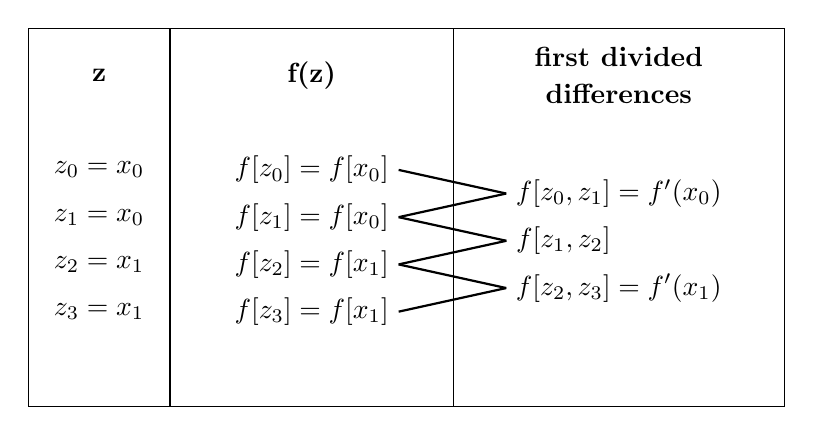
\begin{tikzpicture}[scale=1.2]
\draw (0,0) rectangle (8,4);

% Horizontal lines
% \foreach \y in {1,2,3}
% \draw (0,\y) -- (9,\y);

% Vertical lines
\draw (1.5,0) -- (1.5,4);
\draw (4.5,0) -- (4.5,4);

% Column titles
\node at (0.75,3.5) {\textbf{z}};
\node at (3,3.5) {\textbf{f(z)}};
\node at (6.25,3.7) {\textbf{first divided}};
\node at (6.25,3.3) {\textbf{differences}};
% \node at (8.25,3.7) {\textbf{second divided}};
% \node at (8.25,3.3) {\textbf{differences}};

% Entries for z
\node at (0.75,2.5) {$z_0 = x_0$};
\node at (0.75,2) {$z_1 = x_0$};
\node at (0.75,1.5) {$z_2 = x_1$};
\node at (0.75,1) {$z_3 = x_1$};

% Entries for f(z)
\node (F1) at (3,2.5) {$f[z_0] = f[x_0]$};
\node (F2) at (3,2) {$f[z_1] = f[x_0]$};
\node (F3) at (3,1.5) {$f[z_2] = f[x_1]$};
\node (F4) at (3,1) {$f[z_3] = f[x_1]$};

% First divided differences
\node (1D1) at (6.25,2.25) {$f[z_0,z_1] = f'(x_0)$};
\node (1D2) at (6.25,1.75) {$f[z_1,z_2]\qquad\qquad$};
\node (1D3) at (6.25,1.25) {$f[z_2,z_3] = f'(x_1)$};

\draw[thick] (F1.east) -- (1D1.west);
\draw[thick] (F2.east) -- (1D1.west);
\draw[thick] (F2.east) -- (1D2.west);
\draw[thick] (F3.east) -- (1D2.west);
\draw[thick] (F3.east) -- (1D3.west);
\draw[thick] (F4.east) -- (1D3.west);

% \draw[thick] (1D1.east) -- (1D2.west);
% \draw[thick] (1D2.east) -- (1D3.west);

% Second divided differences
% \node (2D1) at (8.25,2.25) {$f[z_0,z_1,z_2] = f''(x_0)$};
% \node (2D2) at (8.25,1.75) {$f[z_1,z_2,z_3]$};
% \node (2D3) at (8.25,1.25) {$f[z_2,z_3,z_4] = f''(x_1)$};

% \draw[thick] (F1.east) -- (2D1.west);
% \draw[thick] (F2.east) -- (2D1.west);
% \draw[thick] (F3.east) -- (2D2.west);
% \draw[thick] (F4.east) -- (2

\end{tikzpicture}
\end{center}

\subsection{The Hermite Polynomial}

The Hermite polynomial is then defined as

\[
  H(x) = f[z_0] + \sum_{k=1}^{2n+1} f[z_0, \dots, z_k]\prod_{j=0}^{k-1} (x-z_j)
.\]

\section{Splines}

Previously, we saw how to compute an approximation to a function over some
finite interval using a single polynomial. We increased the degree of the
polynomial if we wanted more accuracy.



Even if we enforce the constraint that $f$ and $f'$ agree at the nodes, we still
have the problem that $P_n$ will be expensive to compute for large $n$ and that
for high $n$, the interpolating polynomial can still oscillate wildly.

\section{Splines (15.1)}

Previously, we used a single polynomial to compute an approximation to a
function over some finite interval. We increased the degree of the polynomial if
we wanted more accuracy. However, increasing the degree of the polynomial causes
oscillatory behaviour, and high degree polynomials have the property that a
fluctuation over a small portion of the interval can induce large fluctuations
over the entire interval.

An alternative approach is to divide the interval into subintervals and use a
different, lower degree polynomial in each subinterval. These polynomials are
patched together to give a piecewise polynomial approximation. 

\subsection{Possible Choices}
 
\subsubsection{Piecewise Linear Interpolation}

We join a set of data points by a series of straight lines.

The biggest disadvantage of this approach is that the approximation is typically
not smooth. \ie it is not differentiable at these points, which may not be
satisfactory.

\subsubsection{Piecewise Polynomails of Hermite Type}

*Hermite is pronounced \enquote{her-meat}

If we know the value of a function \textbf{and} it's derivative at each of the
data points, then we could use a Hermite cubic polynomial on each interval
$[x_i, x_{i+1}]$ to approximate the function. Often, however, the derivative of
the function is not known at the data points.

\subsubsection{Piecewise Quadratic Polynomials}

Alternatively, we could join a set of polynomials with quadratic polynomials.
This gives us $3$ arbitrary constants. There will be $2$ conditions to fit the
curve through the endpoints of each interval, but there isn't enough flexibility
to set conditions on the derivative at both endpoints $x$ and $x_n$.

We have enough flexibility to set conditions for the first $n-1$ data points,
but the data point $x_n$ requires four conditions, when we can only provide
three degrees of freedom.

\begin{itemize}
\item $P_0$: 2 endpoint conditions + 1 slope condition
\item $P_1$: 2 endpoint conditions + 1 slope conditions
\item $P_n$: 2 endpoint conditions + 2 slope conditions
\end{itemize}

\subsubsection{Cubic Spline Interpolation}

If we use cubic polynomials between each successive pair of nodes, then there
are four constants and it is possible to ensure that the interpolant

\begin{itemize}
  \item agrees with the function at all the nodes
  \item is continuously differentiable
  \item has continuous second derivatives
\end{itemize}

Given a function $f$ defined on $[a, b]$ and a set of nodes
$a=x_0<x_1<\dots<x_n=b$, a cubic spline interpolant $S$ for $f$ is a function
that satisfies the following:

\begin{itemize}
  \item $S(x) = S_j(x)$ on $[x_j, x_{j+1}]$
  \item $S_j(x_{j+1}) = f(x_{j+1}) = S_{j+1}(x_j)$ splines must pass through the
    data points
  \item $S_j'(x_{j+1}) = S'_{j+1}(x_{j+1})$ first derivative is continuous
  \item $S_j''(x_{j+1}) = S''_{j+1}(x_{j+1})$ second derivative is continuous
\end{itemize}

We also need a boundary condition. Typically one of the following hold in the
problems we will consider: 

\begin{itemize}
  \item $S'(x_0) = f'(x_0)$ and $S'(x_n) = f'(x_n)$ 
    \enquote{Clamped Boundary Conditions}
  \item $S''(x_0) = 0 = S''(x_n)$
    \enquote{Free or Natural Boundary Conditions} \\
    \small{
    *Natural Boundary Conditions tell us that $S$ is not curved at the endpoints.
  }
\end{itemize}

Of course, for the clamped case, we need derivative information, either from the
physics or from some assumption. If there are $(n+1)$ points, the number of
intervals and the number of $S_i(x)$'s are $n:$

\[
  S_i(x) = a_i + b_i (x-x_i) + c_i (x-x_i)^2 + d_i (x-x_i)^3
.\]

Letting $h_i = x_{i+1} - x_i$  we can simplify by substituting $x_{i+1}$ and
$x_i$ into $S_i(x)$, $S_i'(x)$ and $S_i''(x)$. Eliminating the $b_i$ and $d_i$
gives a linear system of equations:

\begin{align*}
&h_{i-1}c_{i-1} + 2(h_{i-1} + h_i)c_i + h_0 c_{i+1} \\
&\quad= \frac{3}{h_i}(a_{i+1}-a_i) - \frac{3}{h_{i-1}}(a_i - a_{i-1})\\
&\quad 1 \leq i \leq n-1
\end{align*}

where the $a_i$ are known

\[
  a_i = f(x_i) \qquad 0 \leq i \leq n-1
.\]

and we define 

\begin{align*}
  a_n &\equiv f(x_n) \\
  b_n &\equiv f'(x_n) \\
  c_n &\equiv \frac{f''(x_n)}{2}
\end{align*}

The $b_i$ and $d_i$ are easily found:

\[
  b_i = \frac{1}{h_i}(a_{i+1} - a_i) - \frac{h_i}{3} (2c_i + c_{i+1}) \quad 0 \leq i \leq n-1
.\]

\[
  d_i = \frac{c_{i+1} - c_i}{3h_i}
.\]

We still need to impose the boundary conditions:

\textbf{Natural Boundary Conditions}
Consider the Natural BC's: $S''(x_0) = S''(x_n) = 0$.

\[
\therefore C_n = 0 \quad\text{(by definition)}
.\]

\[
S_0''(x) = 2C_0 + 6d_0(x-x_0) \therefore S''(x_0) = 2c_0 + 6d_0(x_0-x_0) = 0 =
c_0
.\]

We can derive a matrix equation for the $[c_i]$:

\[
Ax = b
.\]

where 

\[
  A = \begin{bmatrix}
    1 & 0 & 0 & \dots & \dots &  0 \\
    h_0 & 2(h_0+h_1) & h_1 & \ddots & &  \vdots\\
    0 & h_1 & 2(h_1+h_2) & h_2 & \ddots  & \vdots\\
    \vdots & & \ddots & \ddots & \ddots  & \vdots\\
    \vdots & & & h_{n-2} & 2(h_{n-2}+h_{n-1}) & h_{n-1}  \\
    0 & \dots & \dots & 0 & 0 & 1
  \end{bmatrix}
\]

\[
 x=\begin{bmatrix}
 c_0\\
 c_1\\
 \vdots\\
 c_n\\
 \end{bmatrix}
.\]

\[
b=\begin{bmatrix}
0\\
\frac{3}{h_1}(a_2-a_1)-\frac{3}{h_0}(a_1-a_0)\\
\vdots\\
\frac{3}{h_{n-1}}(a_{n}-a_{n-l})-\frac{3}{h_{n-2}}(a_{n-1}-a_{n-2})\\
0
\end{bmatrix}
.\]

There exists a unique solution for the $c_i$'s.

The matrix is strictly diagonally dominant, so it is invertible and a unique
solution for the $c_i$ exists.

First we need a definition and a theorem.

\defn The $n \times n$ matrix $A$ is strictily diagonally dominant if 

\[
  |a_{ii}| > \sum_{j=1; j\neq i}^{n} |a_{ij}|
.\]

holds for each $i = 1, \dots, n$.

\thm A strictly diagonally dominant matrix is invertible.

Also note that the matrix $A$ is \textbf{tridiagonal}: all entires are zero
except for a band which is 3 entries wide centred on the main diagonal.

Solutions to tridiagonal linear systems can be found very efficiently:

*Only O(n) operations are needed using methods we shall discuss later

\textbf{Clamped Boundary Conditions}
We also want to treat clamped boundary conditions:

\[
f'(a) = S'(a) = S_0'(x_0) = b_0 + 2c_0 (x_0-x_0) + 3d_0 (x_0-x_0)^2 = b_0
.\]

but 
\[
  b_{i-1} = \frac{a_i - a_{i-1}}{h_{i-1}} - \frac{h_{i-1}}{3}(2c_{i-1} + c_i)
.\]

\[
\therefore b_0 = \frac{a_1 - a_0}{h_0} - \frac{h_0}{3}(2c_0 + c_1)
.\]

\[
\implies 2h_0c_0 + h_0 c_1 = \frac{3}{h_0}(a_1 - a_0) - 3f'(a)
.\]

Similarly, 

\[
  h_{n-1} c_{n-1} + 2h_{n-1} c_n = 3f'(b) - \frac{3}{h_{n-1}}(a_{n-1} - a_n)
.\]

Once again, we obtain a strictly diagonally dominant linear system

\begin{center}
  $\implies$ A unique solution exists for the $c_i$'s
\end{center}

Furthermore, the system is tridiagonal so it can be solved efficiently for the
coefficients of the spline.


\section{Parametric Curves (C3*2-16.3)}

The interpolating polynomials and splines that we have previously discussed can
only be used to interpolate functions. The techniques can be extended to
represent general curves in space that aren't necessarily functions, or even
curves which self-intersect. %The way we will do this is by ...

Suppose we wish to determine a polynomial or a pieceewise polynomial to connect
the points 

\[
(x_0, y_0), (x_1, y_1), \dots, (x_n, y_n) 
.\]

in the order given.

We can define a parameter $t$ with the interval $[t_0, t_n]$ with
\[
t_0 < t_1 < \dots < t_n
.\]

and construct approximation functions for $x$ and $y$ separately:
\[
x_i = x(t_i), \quad y_i = y(t_i)
.\]

\pagebreak
\Ex
\begin{center}
  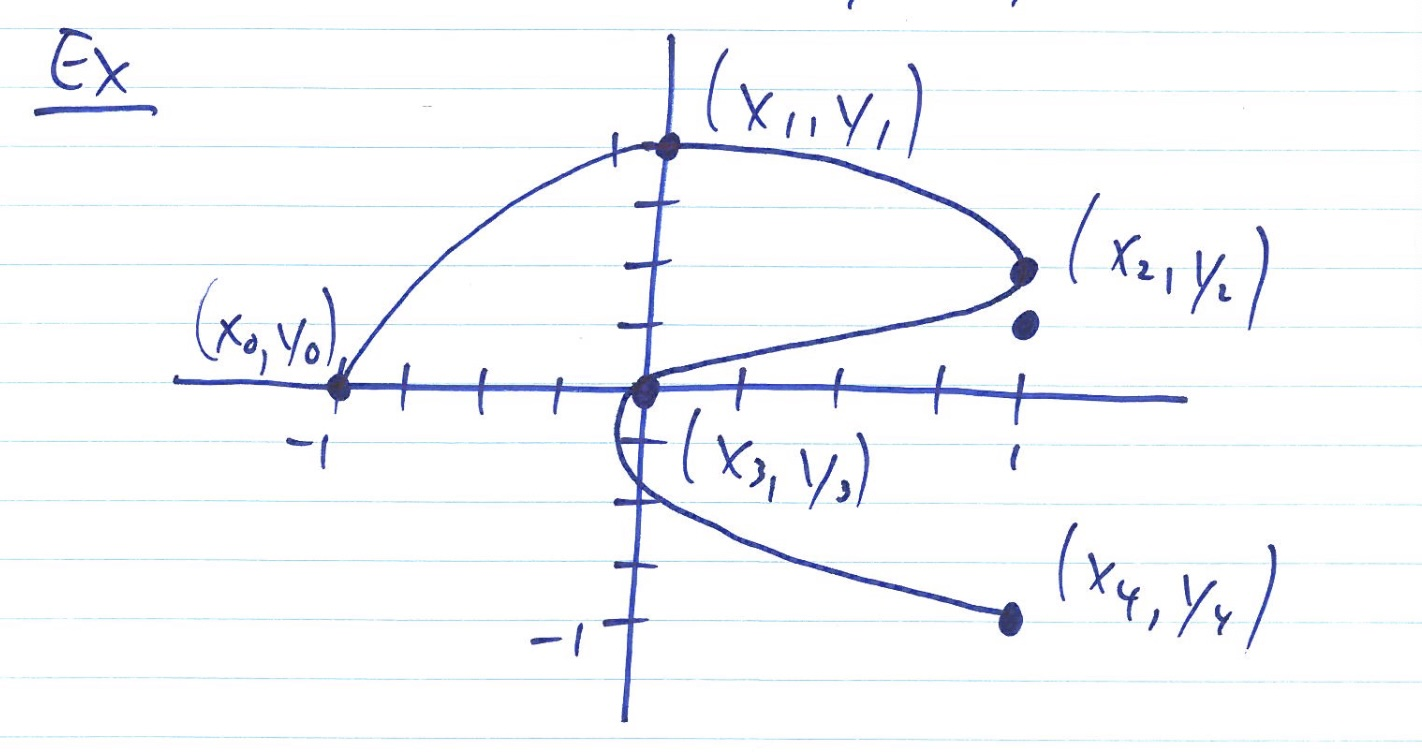
\includegraphics[width=0.8\textwidth]{./assets/parametric_curves_1.jpg}
\end{center}

There is flexibility in choosing the points $t_i$. Suppose we choose them to be
evenly spaced over $[0, 1]$. Then we can write

\[
\begin{array}{c|ccccc}
i & 0 & 1 & 2 & 3 & 4 \\ \hline
t_i & 0 & .25 & .5 & .75 & 1 \\
x_i & -1 & 0 & 1 & 0 & 1 \\
y_i & 0 & 1 & .5 & 0 & -1
\end{array}
\]

We could apply Lagrange interpolation for $x$ (or $y$) as a function of $t$.
The Lagrange Interpolating polynomials for $x$ and $y$ are

\[
x(t) = \left(\left(\left(64\,t - \frac{352}{3}\right)t + 60\right)t - \frac{1}{3}\right)t - 1
\]
\[
y(t) = \left(\left(\left(-\frac{64}{3}t + 48\right)t - \frac{116}{3}\right)t + 11\right)t
\] 

Alternatively, we could use a spline-based interpolation for $x$ and $y$.

Both of these approaches have the disadvantage that moving a single data point
affects the entire curve. We want the geometric property that changing one of
the points on the curve only changes one portion of the curve. \ie we want the
curve to only be affected locally by changes in the data.

\subsection{Piecewise Cubic Hermite Polynomials}
Because we want to avoid global changes, we might use a piecewise cubic Hermite
polynomial, which is just a spline with specific properties. We use one
polynomial for $x$ and one for $y$, both with respecto to $t$.

In other words, we specify the endpoints and the derivatives and the endpoints
to specify each portion of the curve. Thus, changin ga datapoint will only
change the two portions adjacent to the point, which means that smooth curves
can be easily and quickly modified.

\subsubsection{Uniqueness}

Quick answer: No.

\subsubsection{The Derivatives and Tangent Lines (C3*2-16.7)}
Suppose that the endpoints are at $t=0$ and $t=1$, then we only need to satisfy
the conditions on the quotients

\[
\frac{dy}{dx} (t=0) = \frac{y'(0)}{x'(0)}, \quad \frac{dy}{dx} (t=1)
= \frac{y'(1)}{x'(1)}
.\]

The actual values of $x'(0)$ and $y'(0)$ can be scaled by a common factor and
still satisfy these conditions. The larger the scaling factor, the closer the
curve comes to satisfying the tangent line near $(x(0), y(0))$.

A similar situation holds for 

\[
  (x(1), y(1))
.\]

\subsubsection{Guide Points (Cubic Bezier Curves)}
To simplify the process of specifying the slopes and to obtain a unique curve,
commercial software commonly specifies a second point called a
\enquote{guidepoint} which lies on the desired tangent line.

Suppose the endpoints are

\[
  (x(0), y(0)), \text{ and } (x(1), y(1))
.\]

and let the guidepoints be

\[
  (x_0 + \alpha_0, y_0 + \beta_0), \text{ and } (x_1 + \alpha_1, y_1 + \beta_1)
.\]

we will insist that $x$ satisfies

\begin{align*}
  x(0) &= x_0 & x'(0) &= \alpha_0 \\
  x(1) &= x_1 & x'(1) &= \alpha_1
\end{align*}

and that $y$ satisfies

\begin{align*}
  y(0) &= y_0 & y'(0) &= \beta_0 \\
  y(1) &= y_1 & y'(1) &= \beta_1
\end{align*}

Now there is a unique solution for $x$ and $y$:

\begin{align*}
    x(t) &= \left[ 2(x_0 - x_1) + (\alpha_0 + \alpha_1) \right] t^3 \\
         &\quad + \left[ 3(x_1 - x_0) - (\alpha_1 + 2\alpha_0) \right] t^2 \\
         &\quad + \alpha_0 t + x_0
\end{align*}

\begin{align*}
    y(t) &= \left[ 2(y_0 - y_1) + (\beta_0 + \beta_1) \right] t^3 \\
         &\quad + \left[ 3(y_1 - y_0) - (\beta_1 + 2\beta_0) \right] t^2 \\
         &\quad + \beta_0 t + y_0
\end{align*}

Popular graphics programs will typically use a slightly modified form for $x$
and $y$. They use B\'ezier polynomials which scale the derivatives $x'$ and $y'$
by a factor of $\mathbf{3}$ at the endpoints.

\begin{align*}
    x(t) &= \left[ 2(x_0 - x_1) + (\alpha_0 + \alpha_1) \right] t^3 \\
         &\quad + \left[ 3(x_1 - x_0) - (\alpha_1 + 2\alpha_0) \right] t^2 \\
         &\quad + \mathbf{3}\alpha_0 t + x_0
\end{align*}

\begin{align*}
    y(t) &= \left[ 2(y_0 - y_1) + (\beta_0 + \beta_1) \right] t^3 \\
         &\quad + \left[ 3(y_1 - y_0) - (\beta_1 + 2\beta_0) \right] t^2 \\
         &\quad + \mathbf{3}\beta_0 t + y_0
\end{align*}

\subsubsection{Fun Notes}

Generally, given that you don't have two points on the same point, i.e. you
don't have
$
  (x(0), y(0)) = (x(1), y(1))
$,
you can guarantee that the output curve will be continuous with a continuous
derivative. (i.e. $P \in C^1[a, b]$).

\section{Numerical Differentiation (C4*1-17.1)}

We also need to approximate the derivatives of functions. One approach is to
differentiate Lagrange polynomial approximations.

Suppose $x_0, x \in (a, b)$ and $f\in C^2[a,b]$.

Now

\begin{align*}
    f(x) &= P_{0,1}(x) + \frac{1}{2!} (x - x_0)(x - x_1) f''(\xi(x)) \\
         &= \frac{f(x_0)(x - x_1)}{x_0 - x_1} + \frac{f(x_1)(x - x_0)}{x_1 - x_0} 
         + \frac{(x - x_0)(x - x_1)}{2!} f''(\xi(x)) \\
         &\text{where } \xi(x) \in [a, b]
\end{align*}

Now differentiate:

\begin{align*}
    f'(x) &= \frac{f(x_1) - f(x_0)}{x_1 - x_0} + D_x \left[ \frac{(x - x_0)(x - x_1)}{2!} f''(\xi(x)) \right] \\
          &= \frac{f(x_1) - f(x_0)}{x_1 - x_0} + \frac{2 (x - x_0)(x - x_1)}{2} f''(\xi(x)) \\
          &\quad + \frac{(x - x_0)(x - x_1)}{2} D_x \left( f''(\xi(x)) \right)
\end{align*}

\subsection{More remarks}
Chapter 4 also considers numerical integration. We know how to integrate
polynomials, so we can just integrate the lagrange polynomial and call it a day.


\section*{Key Takeaways from this Lecture}

Be aware that most of what we did in this chapter is looking over formulas for
approximating derivatives. So this entire notes package is just math. The key
takeaways are just point forms of what we went over.

\begin{enumerate}
  \item Numerical Differentiation (\ref{sec:numerical_differentiation})
    \begin{enumerate}[label=(\alph*)]
      \item We approximate derivatives using interpolation of easier functions 
        (\ex Lagrange polynomials)
      \item Simplest case: using two points to approximate the first derivative
      \item The \textbf{Forward Difference Formula} (for $h>0$) and
        \textbf{Backward Difference Formula} (for $h<0$) are basic numerical
        differentiation methods \eqref{eq:difference_formula}
    \end{enumerate}
  \item More General Approximation Formulas (\ref{sec:more_general_approximation_formulas})
    \begin{enumerate}[label=(\alph*)]
      \item Using $(n+1)$-point formulas, we get more accurate derivative
        approximations
      \item These formulas all follow from differentiating Lagrange polynomials
      \item Three, five and higher-order point formulas are commonly used
      \item Formula reference: \eqref{eq:three_point_formula}. The error term
        depends on the highest derivative of $f(x)$ and the spacing of the
        nodes.
    \end{enumerate}
  \item Equally Spaced Three-Point Formulas (\ref{sec:equally_spaced_three_point_formulas})
    \begin{enumerate}[label=(\alph*)]
      \item When the points are evenly spaced, the formulas for approximating
        derivatives become \eqref{eq:three_point_formula_1}, \eqref{eq:three_point_formula_2}
        and \eqref{eq:three_point_formula_3}
      \item These three formulas correspond to 
        \begin{enumerate}
          \item Forward Difference (uses two points ahead)
          \item Centered Difference (uses one point in front and one point behind)
          \item Backward Difference (uses two points behind)
        \end{enumerate}
      \item Check out Example~1 (Section~\ref{sec:example_1})
    \end{enumerate}
  \item Second Derivative Approximation (\ref{sec:second_derivative_approximation})
    \begin{enumerate}[label=(\alph*)]
      \item We approximate $f''(x)$ by using function values at three points.
      \item The formulas are derived using Taylor series expansion: \eqref{eq:second_derivative_approximation}
    \end{enumerate}
  \item Remarks on Error \ref{sec:remarks_on_error}
    \begin{enumerate}[label=(\alph*)]
      \item \textbf{Small $h$ leads to large roundoff errors.}
      \item Since numerical differentiation involves dividing by $h$ and higher
        orders of $h$, extremely small $h$ values can exaggerate computational
        errors.
      \item Typically, beyond $h\approx 10^{-6}$, roundoff errors dominate the
        calculation.
    \end{enumerate}
  \item Richardson's Extrapolation \ref{sec:richardson_extrapolation}
    \begin{enumerate}[label=(\alph*)]
      \item If the error depends on some parameter (such as the step size $h$)
        and the dependency of the error is predictable (we know the erroe
        behaviour), we can extrapolate to obtain more accurate approximations.
      \item We use multiple approximations at different step sizes and
        \textbf{combine them to cancel error terms}.
      \item There's a step by step process here: \eqref{eq:*}, \eqref{eq:**},
        \eqref{eq:?}, \eqref{eq:***}, \eqref{eq:****}, \eqref{eq:???}
      \item This process gives increasing accuracy with each step.
    \end{enumerate}
  \item Final Remarks
    \begin{enumerate}[label=(\alph*)]
      \item Numerical differentiation can \textbf{amplify errors}, so careful
        step-size selection is crucial.
      \item Centered difference methods are generally more accurate than forward
        or backward differences.
      \item \textbf{Richardson's Extrapolation} is a systematic way to improve
        accuracy.
      \item In numerical integration (covered in a later part of this chapter),
        we will integrate the Lagrange polynomial instead of differentiating it.
    \end{enumerate}
  \item Also check out Random Stuff Steve said during lecture \ref{sec:random_stuff}
\end{enumerate}

\section{Numerical Differentiation (C4*1-17.1)}\label{sec:numerical_differentiation}

We also need to approximate the derivatives of functions. One approach is to
differentiate Lagrange polynomial approximations.

Suppose $x_0, x \in (a, b)$ and $f\in C^2[a,b]$.

Now

\begin{align*}
    f(x) &= P_{0,1}(x) + \frac{1}{2!} (x - x_0)(x - x_1) f''(\xi(x)) \\
         &= \frac{f(x_0)(x - x_1)}{x_0 - x_1} + \frac{f(x_1)(x - x_0)}{x_1 - x_0} 
         + \frac{(x - x_0)(x - x_1)}{2!} f''(\xi(x)) \\
         &\text{where } \xi(x) \in [a, b]
\end{align*}

Now differentiate:

\begin{align*}
    f'(x) &= \frac{f(x_1) - f(x_0)}{x_1 - x_0} + D_x \left[ \frac{(x - x_0)(x - x_1)}{2!} f''(\xi(x)) \right] \\
          &= \frac{f(x_1) - f(x_0)}{x_1 - x_0} + \frac{2 (x - x_0)(x - x_1)}{2} f''(\xi(x)) \\
          &\quad + \frac{(x - x_0)(x - x_1)}{2} D_x \left( f''(\xi(x)) \right)
\end{align*}

We only care about the derivatives at the nodes $x_0, x_1$. The last error term
becomes zero.

\pagebreak
For example, at $x=x_0$,

\[
f'(x_0) = \frac{f(x_1) - f(x_0)}{x_1 - x_0} - \frac{(x_0 - x_1)}{2} f''(\xi)
.\]

Typically, we set $x_1 = x_0+h$, then
\begin{equation}
  f'(x_0) = \frac{f(x_0+h) - f(x_0)}{h} - \frac{h}{2} f''(\xi(x_0))
  \label{eq:difference_formula}
\end{equation}

This is known as a \uline{forward difference formula} if $h>0$ and a \uline{backward
difference formula} if $h<0$. We can derive more general approximation formulas:

\subsection{More General Approximation Formulas (17.3)}\label{sec:more_general_approximation_formulas}

Suppose $x_0, x_1, \dots x_n \in (a,b)$ and $f\in C^{n+1}[a,b]$. Now

\begin{align*}
  f(x) &= \sum_{k=0}^n f(x_k) L_k(x) \\
  &\quad+ \frac{(x-x_0)\dots (x-x_n)}{(n+1)!} f^{(n+1)}(\xi(x))
\end{align*}

for some $\xi(x) \in [a,b]$

Differentiate and evaluate at $x=x_j$:

\begin{align*}
  f'(x_j) &= \sum_{k=0}^n f(x_k) L_k'(x_j) \\
          &\quad+ \frac{f^{(n+1)}(\xi(x_j))}{(n+1)!} \prod_{k=0; k\neq j}^{n} (x_j - x_k)
          \label{eq:three_point_formula}
\end{align*}

This is an $(n+1)$ point formula for $f'(x_j)$ since we use the $(n+1)$ values
$f(x_k); k=0,\dots,n$. Two, three and five point formulas are hte most commonly
used formulas.

\subsubsection{Three Point Formulas (17.4)}

Consider $3$ point formulas with $x_0, x_1$ and $x_2$.

Given \( n = 2 \):

\[
L_0(x) = \frac{(x - x_1)(x - x_2)}{(x_0 - x_1)(x_0 - x_2)}
\]

Taking the derivative:

\[
L_0'(x) = \frac{2x - x_1 - x_2}{(x_0 - x_1)(x_0 - x_2)}
\]

Similarly,

\begin{align*}
    L_1'(x) &= \frac{2x - x_0 - x_2}{(x_1 - x_0)(x_1 - x_2)} \\[10pt]
    L_2'(x) &= \frac{2x - x_0 - x_1}{(x_2 - x_0)(x_2 - x_1)}
\end{align*}

\noindent and

\begin{align*}
    f'(x_j) &= f[x_0] \left[ \frac{2x_j - x_1 - x_2}{(x_0 - x_1)(x_0 - x_2)} \right] \\[10pt]
    &\quad + f[x_1] \left[ \frac{2x_j - x_0 - x_2}{(x_1 - x_0)(x_1 - x_2)} \right] \\[10pt]
    &\quad + f[x_2] \left[ \frac{2x_j - x_0 - x_1}{(x_2 - x_0)(x_2 - x_1)} \right] \\[10pt]
    &\quad + \frac{1}{6} f^{(3)}(\xi_j) \prod_{\substack{k=0 \\ k \neq j}}^{2} (x_j - x_k)
\end{align*}

These simplify considerably when nodes are equally spaced:

\subsubsection{Equally Spaced Three Point Formulas (17.5)}\label{sec:equally_spaced_three_point_formulas}

Given:
\[
x_1 = x_0 + h, \quad x_2 = x_0 + 2h
\]

\begin{align}
    f'(x_0) &= \frac{1}{h} \left[ -\frac{3}{2} f(x_0) + 2f(x_0 + h) - \frac{1}{2} f(x_0 + 2h) \right] 
    + \frac{h^2}{3} f^{(3)}(\xi_0)
    \label{eq:three_point_formula_1}\\[10pt] 
    f'(x_1) &= \frac{1}{h} \left[ -\frac{1}{2} f(x_1 - h) + \frac{1}{2} f(x_1 + h) \right] 
    - \frac{h^2}{6} f^{(3)}(\xi_1) 
    \label{eq:three_point_formula_2}\\[10pt]
    f'(x_2) &= \frac{1}{h} \left[ \frac{1}{2} f(x_2 - 2h) - 2f(x_2 - h) + \frac{3}{2} f(x_2) \right] 
    + \frac{h^2}{3} f^{(3)}(\xi_2)
    \label{eq:three_point_formula_3}
\end{align}

For convenience, replace $x_1$ and $x_2$ by $x_0$. This gives 3 formulas for
approximating $f'(x_0)$.

\begin{align*}
    f'(x_0) &= \frac{1}{h} \left[ -\frac{3}{2} f(x_0) + 2 f(x_0 + h) - \frac{1}{2} f(x_0 + 2h) \right] 
    + \frac{h^2}{3} f^{(3)}(\xi_0) \\[10pt]
    f'(x_0) &= \frac{1}{h} \left[ -\frac{1}{2} f(x_0 - h) + \frac{1}{2} f(x_0 + h) \right] 
    - \frac{h^2}{6} f^{(3)}(\xi_1) \\[10pt]
    f'(x_0) &= \frac{1}{h} \left[ \frac{1}{2} f(x_0 - 2h) - 2 f(x_0 - h) + \frac{3}{2} f(x_0) \right] 
    + \frac{h^2}{3} f^{(3)}(\xi_2)
\end{align*}

Formula 1 uses two points ahead, formula 2 uses one point in front and one point
behind, and formula 3 uses two points behind.

\pagebreak
\subsubsection{Example 1 (17.5.1)}\label{sec:example_1}

\Ex use the most appropriate three-point formula to determine approximatinos
that will complete the following table:

\begin{table}[h]
    \centering
    \begin{tabular}{|c|c|c|}
        \hline
        $x$  & $f(x)$    & $f'(x)$ \\ 
        \hline
        1.1  & 9.025013  &  \\ 
        1.2  & 11.02318  &  \\ 
        1.3  & 13.46374  &  \\ 
        1.4  & 16.44465  &  \\ 
        \hline
    \end{tabular}
    % \caption{Table of values for $x$, $f(x)$, and $f'(x)$.}
    % \label{tab:values}
\end{table}

\uline{ANSWER: (17.6)}

We only have data in $[1.1, 1.4]$, and no data before or after this interval.
So, for $f'(1.1)$ we use formula 1. For $f'(1.2)$ we can use formula 2 or
formula 1, but since formula 2 has a smaller error, we choose it. We do the same
for $f'(1.3)$. For $f'(1.4)$ we use formula 3, since we only have data behind,
and no available data ahead.

\begin{align*}
    f'(1.1) &\approx \frac{1}{2(0.1)} \left[ -3f(1.1) + 4f(1.2) - f(1.3) \right] = 17.769705 \\[10pt]
    f'(1.2) &\approx \frac{1}{2(0.1)} \left[ f(1.3) - f(1.1) \right] = 22.193635 \\[10pt]
    f'(1.3) &\approx \frac{1}{2(0.1)} \left[ f(1.4) - f(1.2) \right] = 27.107350 \\[10pt]
    f'(1.4) &\approx \frac{1}{2(0.1)} \left[ f(1.2) - 4f(1.3) + f(1.4) \right] = 32.510850
\end{align*}

\textit{*these are OCR'd through ChatGPT. They may be wrong.}

Notice that at the endpoints we must use one sided difference formulas. In the
interior, we used centered differencing. Centered differences often have a
smaller error constant when $f$ is smooth, and they require fewer operations to
compute, but they cannot be used at the endpoints.

\subsubsection{The Second Derivative of $f$ (17.8)}\label{sec:second_derivative_approximation}
Approximations to higher order derivatives may also be found based on function
values. Consider finding the second derivative of $f$.

\begin{align*}
    f(x_0 + h) &= f(x_0) + f'(x_0) h + \frac{1}{2} f''(x_0) h^2 + \frac{1}{6}
    f'''(x_0) h^3 + \frac{1}{24} f^{(4)}(\xi_1) h^4 \\
    f(x_0 - h) &= f(x_0) - f'(x_0) h + \frac{1}{2} f''(x_0) h^2 - \frac{1}{6}
    f'''(x_0) h^3 + \frac{1}{24} f^{(4)}(\xi_{-1}) h^4
\end{align*}

\noindent where \( x_0 - h < \xi_{-1} < x_0 < \xi_{1} < x_0 + h \).

Summing:
\begin{equation}
    f(x_0 + h) + f(x_0 - h) = 2f(x_0) + f''(x_0) h^2 + \frac{h^4}{24} \left[ f^{(4)}(\xi_1) + f^{(4)}(\xi_2) \right]
    \label{eq:second_derivative_approximation}
\end{equation}

We assume \( f^{(4)} \) is continuous on \( [x_0 - h, x_0 + h] \).

Since
\(
\displaystyle\frac{1}{2} \left[ f^{(4)}(\xi_1) + f^{(4)}(\xi_{-1}) \right]
\)
is between \( f^{(4)}(\xi_1) \) and \( f^{(4)}(\xi_{-1}) \), the 
\textit{intermediate value theorem} implies that there is a number
\( \xi \) between \( \xi_1 \) and \( \xi_2 \) such that
\[
  f^{(4)}(\xi) = \frac{1}{2} \left[ f^{(4)}(\xi_1) + f^{(4)}(\xi_{-1}) \right].
\]

Thus,
\begin{align*}
    f(x_0 + h) + f(x_0 - h) &= 2 f(x_0) + f''(x_0) h^2 + \frac{h^4}{24} f^{(4)}(\xi).
\end{align*}

\noindent Therefore,
\begin{align*}
    f''(x_0) &= \frac{1}{h^2} \left[ f(x_0 - h) - 2 f(x_0) + f(x_0 + h) \right] - \frac{h^2}{24} f^{(4)}(\xi).
\end{align*}

\subsubsection{Remarks on Error (17.9)}\label{sec:remarks_on_error}

Notice that all the differentiation formulas divide by some power of $h$.
Division by small numbers tends to exaggerate roundoff error, but this is an
effect that cannot be entirely avoided in numerical differentiation. Thus we do
not want to take $h$ to be too small because then the roundoff errors will
dominate the calculation.

The exact value at which $h$ becomes too small depends on the scaling of your
problem and your specific function $f$. However, for most problems, scaled
nicely, you will start to see roundoff errors at around $h=10^{-6}$.

\section{Richardson's Extrapolation (C4*1-17.10)}\label{sec:richardson_extrapolation}

When the error depends on some parameter such as the step size $h$ and the
dependency is predictable, we can often derive higher order accuracy from low
order formulas. To illustrate the procedure, assume we have an approximation
$N(h)$ to some quantity $M$. Assume this approximation has an order $h$
truncation error and that we know the expression for the first few terms of the
trunction error,

\begin{equation}
M = N(h) + k_1h + k_2h^2 + k_3h^3 + \dots
\label{eq:*}
\end{equation}

\noindent where the $k_i$'s are constants, $h$ is a positive parameter and
$N(h)$ is an $O(h)$ approximation to $M$. We can repeat the calculation with a
parameter $\frac{h}{2}$. Now:

\begin{equation}
M=N(\frac{h}{2}) + \frac{k_1}{2}h + \frac{k_2}{4}h^2 + \frac{k_3}{8}h^3 + \dots
\label{eq:**}
.\end{equation}

We want to obtain a higher order method by using some combination of these
results. 

Subctracting \eqref{eq:*} from twice \eqref{eq:**} gives:

\begin{equation}
  M = [2N(\frac{h}{2}) - N(h)] + k_2(\frac{h^2}{2} - h^2) + k_3
  (\frac{h^3}{4}-h^3) + \dots
  \label{eq:?}
\end{equation}

which is an $O(h^2)$ approximation formula for $M$. For ease of notiation, 

\[
\text{Let } N_2(h) = 2N(\frac{h}{2}) - N(h)
.\]

Now 

\begin{equation}
  M = N_2(h) - \frac{1}{2} k_2 h^2 - \frac{3}{4} k_3 h^3 - \dots
  \label{eq:***}
\end{equation}

We can repeat this calculation with $\frac{h}{2}$:

Now 

\begin{equation}
  M = N_2(\frac{h}{2}) -\frac{1}{8} k_2 h^2 - \frac{3k^3}{32}h^3 - \dots
  \label{eq:****}
  \end{equation}

We want to eliminate the $h^2$ term. We can do this by subtracting four times 
\eqref{eq:***} from \eqref{eq:****}, which gives:

\begin{equation}
  3M = 4N_2(\frac{h}{2}) -N_2(h) + \frac{3k_3}{8}h^3 + \dots
  \label{eq:???}
\end{equation}

which gives an $O(h^3)$ formula for approximating $M$. 

\begin{align*}
    M &= N_3(h) + \frac{1}{3} J_3 h^3 + \dots
\end{align*}

where
\begin{align*}
    N_3(h) &= \frac{4}{3} N_2 \left(\frac{h}{2}\right) - \frac{1}{3} N_2(h).
\end{align*}

Similarly, an \( O(h^4) \) approximation can be derived as:
\begin{align*}
    N_4(h) &= N_3 \left(\frac{h}{2}\right) + \frac{N_3(h/2) - N_3(h)}{7}.
\end{align*}

And an \( O(h^5) \) approximation:
\begin{align*}
    N_5(h) &= N_4 \left(\frac{h}{2}\right) + \frac{N_4(h/2) - N_4(h)}{15}.
\end{align*}

Generally, if \( M \) can be written as:
\begin{align*}
    M = N(h) + \sum_{j=1}^{m-1} K_j h^j + O(h^m),
\end{align*}
then for each \( j = 2, 3, \dots, m \), we have an \( O(h^j) \) approximation of the form:
\begin{align*}
    N_j(h) = N_{j-1} \left(\frac{h}{2}\right) + \frac{N_{j-1} \left(\frac{h}{2}\right) - N_{j-1}(h)}{2^{j-1} - 1}.
\end{align*}

\subsection{More remarks - things that Steve said during lecture}\label{sec:random_stuff}
Chapter 4 also considers numerical integration. We know how to integrate
polynomials, so we can just integrate the lagrange polynomial and call it a day.


\section{Overview}

The most important parts of this lecture are the following:

\begin{enumerate}
\item \textbf{Richardson's Extrapolation}: A method for obtaining higher order
  accuracy from lower order formulas. link: \ref{sec:richardson_extrapolation}
  \begin{enumerate}
    \item \ref{sec:building_the_extrapolation_table} illustrates the procedure of
      building the richardson extrapolation table.
    \item \ref{sec:richardson_extrapolation_example} illustrates the use of
      Richardson's Extrapolation to obtain a higher order approximation to the
      integral of $\sin x$.
  \end{enumerate}
\item \textbf{Numerical Integration}: A method for evaluating the definite
  integral of a function that has no explicit antiderivative or whose antiderivative
  is not easy to obtain. link: \ref{sec:numerical_integration}
  \begin{enumerate}
    \item \ref{sec:two_point_integration} illustrates the procedure of using a
      2 point integration formula.
    \item \ref{sec:weighted_mean_value_theorem} illustrates the procedure of
      using the weighted mean value theorem for integrals.
    \item \ref{sec:three_point_integration} illustrates the procedure of using a
      3 point integration formula.
  \end{enumerate}
\end{enumerate}

\pagebreak
\section{Richardson's Extrapolation (C4*1-17.10)}\label{sec:richardson_extrapolation}

When the error depends on some parameter such as the step size $h$ and the
dependency is predictable, we can often derive higher order accuracy from low
order formulas. To illustrate the procedure, assume we have an approximation
$N(h)$ to some quantity $M$. Assume this approximation has an order $h$
truncation error and that we know the expression for the first few terms of the
trunction error,

\begin{equation}
M = N(h) + k_1h + k_2h^2 + k_3h^3 + \dots
\label{eq:*}
\end{equation}

\noindent where the $k_i$'s are constants, $h$ is a positive parameter and
$N(h)$ is an $O(h)$ approximation to $M$. We can repeat the calculation with a
parameter $\frac{h}{2}$:

\begin{equation}
M=N\left(\frac{h}{2}\right) + \frac{k_1}{2}h + \frac{k_2}{4}h^2 + \frac{k_3}{8}h^3 + \dots
\label{eq:**}
.\end{equation}

We want to obtain a higher order method by using some combination of these
results. 
Subtracting \eqref{eq:*} from twice \eqref{eq:**} gives:

\begin{equation}
  M = \left[2N\left(\frac{h}{2}\right) - N(h)\right] + k_2\left(\frac{h^2}{2} 
  - h^2\right) + k_3 \left(\frac{h^3}{4}-h^3\right) + \dots
  \label{eq:?}
\end{equation}

\noindent
which is an $O(h^2)$ approximation formula for $M$. For ease of notiation, 

\[
\text{Let } N_2(h) = 2N\left(\frac{h}{2}\right) - N(h)
.\]

% \begin{minipage}{\textwidth}
\noindent
Generally, if $M$ can be written as

\[
  M = N(h) + \sum_{j=1}^{m-1} K_j h^j + O(h^m),
.\]

\noindent
then for each $j = 2, 3, \dots, m$, we have an $O(h^j)$ approximation of the form

\[
  N_j(h) = N_{j-1} \left(\frac{h}{2}\right) + \frac{N_{j-1} \left(\frac{h}{2}\right) - N_{j-1}(h)}{2^{j-1} - 1}.
.\]
% \end{minipage}

In practice, because of how $N_j$ is defined, higher order approximations can 
be systematically derived from lower order approximations.

\subsubsection{Building the Extrapolation Table (18.1)}\label{sec:building_the_extrapolation_table}

\begin{center}
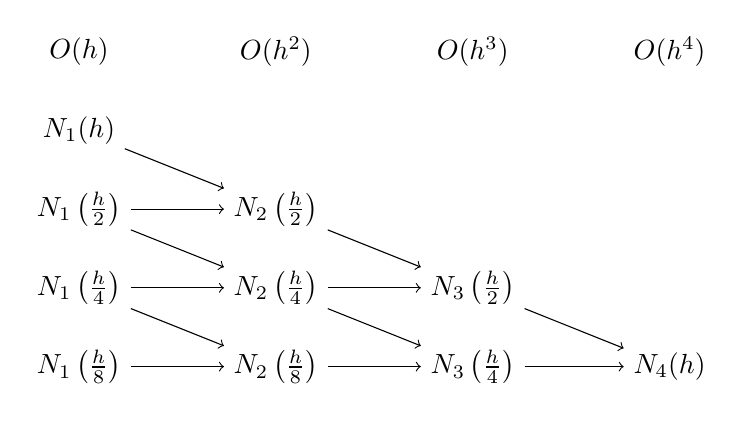
\begin{tikzpicture}[node distance=1cm, font=\sffamily]
  % Nodes
  \node (Oh) {$O(h)$};
  \node[right of=Oh, xshift=1.5cm] (Oh2) {$O(h^2)$};
  \node[right of=Oh2, xshift=1.5cm] (Oh3) {$O(h^3)$};
  \node[right of=Oh3, xshift=1.5cm] (Oh4) {$O(h^4)$};

  % First column nodes
  \node[below of=Oh] (N1h) {$N_{1}(h)$};
  \node[below of=N1h] (N1h2) {$N_{1}\left(\frac{h}{2}\right)$};
  \node[below of=N1h2] (N1h4) {$N_{1}\left(\frac{h}{4}\right)$};
  \node[below of=N1h4] (N1h8) {$N_{1}\left(\frac{h}{8}\right)$};

  % Second column nodes
  \node[right of=N1h2, xshift=1.5cm] (N2h2) {$N_{2}\left(\frac{h}{2}\right)$};
  \node[right of=N1h4, xshift=1.5cm] (N2h4) {$N_{2}\left(\frac{h}{4}\right)$};
  \node[right of=N1h8, xshift=1.5cm] (N2h8) {$N_{2}\left(\frac{h}{8}\right)$};

  % Third column nodes
  \node[right of=N2h4, xshift=1.5cm] (N3h2) {$N_{3}\left(\frac{h}{2}\right)$};
  \node[right of=N2h8, xshift=1.5cm] (N3h4) {$N_{3}\left(\frac{h}{4}\right)$};

  % Fourth column node
  \node[right of=N3h4, xshift=1.5cm] (N4h) {$N_{4}(h)$};

  % Arrows
  \draw[->] (N1h2) -- (N2h2);
  \draw[->] (N1h2) -- (N2h4);
  \draw[->] (N1h) -- (N2h2);
  \draw[->] (N1h4) -- (N2h4);
  \draw[->] (N1h8) -- (N2h8);
  \draw[->] (N2h2) -- (N3h2);
  \draw[->] (N3h2) -- (N4h);
  \draw[->] (N1h4) -- (N2h8);
  \draw[->] (N2h4) -- (N3h4);

  \draw[->] (N2h4) -- (N3h2);
  \draw[->] (N2h8) -- (N3h4);
  

  \draw[->] (N3h4) -- (N4h);
\end{tikzpicture}
\end{center}

The cost of building the extrapolation table is $O(n)$ where $n$ is the inverse 
degree of the error term $(O(h^n))$. Each subsequent iteration of $N$ is defined
solely by its previous iteration, therefore, the cost of building the
extrapolation is the number of initial calculations of $N_1$ required to build
out the table. Some pitfalls of this approach is that the calculation of
$N_{j+1}$ requires a subtraction of two numbers that get closer and closer as
the degree of the error term increases. This is a problem for higher order
calculations, as you may run out of precision and introduce substantial machine
error.

Extrapolation can be used whenever the truncation error for a formula has the
form

\[
  \sum_{j=1}^{m-1} K_j h^{\alpha_j} + O(h^{\alpha_m})
.\]

\noindent
for constants $K_J$ and $\alpha_1 < \alpha_2 < \dots < \alpha_m$.

\subsubsection{When $N_j(h)$ is an $O(h^{2j})$ approximation}\label{sec:richardson_extrapolation_when_n_j_is_o_h_2j}
Suppose $N_j(h)$ is an $O(h^{2j})$ approximation of $M$. Then, from the
definition:

\begin{align}
  M &= N_j(h) + O(h^{2j}) \qquad \text{we add another term of } M \text{:} \\
    &= N_j(h) + k_j(h^{2j}) + O(h^{2j+2}) \label{eq:diamond} \\
    &= N_j(\frac{h}{2}) + k_jh^{2j} + O(h^{2j+2}) \label{eq:2diamond}
\end{align}

$2^{2j}$ \eqref{eq:diamond} $-$ \eqref{eq:2diamond} gives:

\begin{equation*}
  M = N_j(\frac{h}{2}) + \frac{N_j(\frac{h}{2})-N_j(h)}{2^{2j-1}} + O(h^{2j+2})
\end{equation*}

\[
  \boxed{\therefore 
    N_{j+1}(h) \equiv N_j\left(\frac{h}{2}\right) 
    + \frac{N_j\left(\frac{h}{2}\right)-N_j(h)}{4^{j-1}}
  }
.\]

\noindent
is an $O(h^{2j+2})$ approximation of $M$. Then, the table becomes

\begin{center}
  \centering
  \begin{tabular}{cccc}
    $O(h^2)$ & $O(h^4)$ & $O(h^6)$ & $O(h^8)$
  \end{tabular}
\end{center}

\subsection{Richardson's Extrapolation Example (18.1)}\label{sec:richardson_extrapolation_example}

\Ex The following data gives approximations to the integral 

\begin{equation}
  M = \int_0^\infty \sin x \, dx
\end{equation}

\begin{align*}
N_{1}\left(\frac{h}{2}\right) = 1.570796,\quad 
N_{1}\left(\frac{h}{2}\right) = 1.896119\\[6pt]
N_{1}\left(\frac{h}{4}\right) = 1.974232,\quad 
N_{1}\left(\frac{h}{8}\right) = 1.993570
\end{align*}

Assuming 

\[
M = N_1(h) + K_1h^2 + K_2h^4 + k_3h^6 + k_4h^8 + O(h^{10})
.\]

construct an extrapolation table to determine $N_4(h)$.

\soln (from text)

\pagebreak
\section{Numerical Integration (18.4)}\label{sec:numerical_integration}

We often need to evaluate the definite integral of a function that has no
explicit antiderivative or whose antiderivative is not easy to obtain. The usual
strategy in developing formulas for numerical integration is similar to that for
numerical differentiation. We pass a polynomial through points defined by the
function and then integrate this polynomial approximation for the function. This
permist us to use a function known only as a table of values. We get an
expression for the error by integrating the error for our interpolating
polynomial. As we progress, we will eventually turn to splitting our function
into sub-intervals and using methods similar to spline interpolation to
integrate each sub-interval.

\subsection{2-Point Integration Formula (18.5)}\label{sec:two_point_integration}

Suppose we use a 2 point integration formula:

\begin{center}
  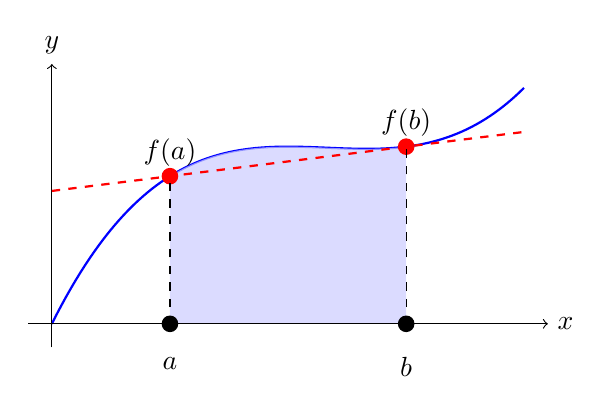
\begin{tikzpicture}[scale=3]
    % Define the function
    \def\f(#1){0.5*(#1)^3 - 1.75*(#1)^2 + 2*(#1)}

    % Define points
    \def\a{0.5}
    \def\b{1.5}

    % Draw the function
    \draw[thick, blue, domain=0:2, samples=100] plot (\x, {\f(\x)});
    % \draw[thick, red, domain=0:2, samples=100] plot (\x, )


    % Shade region between a and b
    \fill[blue!20, opacity=0.7] (\a,0) -- plot[domain=\a:\b, samples=50] (\x, {\f(\x)}) -- (\b,0) -- cycle;

    % Draw axes
    \draw[->] (-0.1,0) -- (2.1,0) node[right] {\(x\)};
    \draw[->] (0,-0.1) -- (0,1.1) node[above] {\(y\)};

    % Dots at the required points
    \foreach \x in {\a, \b} {
        \fill (\x, 0) circle (1pt);
    }
    \foreach \x in {\a, \b} {
      \fill[red] (\x, {\f(\x)}) circle (1pt);
    }

    \draw[dashed] (\a,0) -- (\a, {\f(\a)});
    \draw[dashed] (\b,0) -- (\b, {\f(\b)});
    % \draw[dashed] (\c,0) -- (\c, {\f(\c)});
    \draw[thick, red, dashed, domain=0:2, samples=100] plot (\x, {0.75 + 0.125 * (\x - 1.5)}); % Tangent line

    % Labels for the points
    \node[below] at (\a, -0.1) {\(a\)};
    \node[below] at (\b, -0.1) {\(b\)};
    % \node[below] at (\c, 0) {$\displaystyle\frac{a+b}{2}$};
    \node[above] at (\a, {\f(\a)}) {\(f(a)\)};
    \node[above] at (\b, {\f(\b)}) {\(f(b)\)};
  \end{tikzpicture}
\end{center}


Let $x_0 = a$, $x_1 = b$, $h=b-1$

The linear Lagrange polynomial passing through $(x_0, f(x_0))$ and $(x_1, f(x_1))$ 
is 

\[
P_1(x) = \frac{(x-x_1)(x-x_0)}{f(x_0)} + \frac{(x-x_0)}{(x_1-x_0)} f(x_1)
.\]

and

\begin{align*}
  \int_a^b f(x) \, dx &= \int_{x_0}^{x_1} P_1(x) \, dx +\frac{1}{2}\int_{x_0}^{x}
  f''\left(\xi(x)\right)(x - x_0)(x - x_1)\,dx \\
  &=  \left.\frac{(x - x_1)^2}{2(x_0 - x_1)}f(x_0) + \frac{(x - x_0)^2}{2(x_1 - x_0)}f(x_1)\right|_{x_0}^{x_1} + \text{error}\\[10pt]
  &= \frac{h}{2}\left(f(x_0) + f(x_1)\right) + \text{error}.
\end{align*}

To evaluate the error we will need the \textbf{Weighted Mean Value Theorem for
Integrals}.

\subsubsection{Weighted Mean Value Theorem for Integrals (18.6)}\label{sec:weighted_mean_value_theorem}

If $f\in C[a,b]$, the Riemann Integral of $g$ exists on $[a,b]$ and $g(x)$ does
not change sign on $[a,b]$ then there exists a number $c \in (a,b)$ such that

\[
  \int_a^b f(x) g(x) \, dx = f(c) \int_a^b g(x) 
.\]

\hrule

\begin{align*}
  \text{error} &= \frac{1}{2}\int_{x_0}^{x_1} f''\left(\xi(x)\right)(x - x_0)(x - x_1)\,dx \\
               &= \frac{1}{2} f''(\xi)\int_{x_0}^{x_1}(x - x_0)(x - x_1)\,dx \quad\text{[$\xi$ some number in $(x_0,x_1)$]}\\[6pt]
               &= \frac{1}{2}f''(\xi)\left[\frac{x^3}{3}-\frac{(x_1 + x_0)}{2}x^2+x_0x_1 x\right]_{x_0}^{x_1}\\[6pt]
               &= -\frac{h^3}{12}f''(\xi)
\end{align*}


\[
  \text{Thus } \boxed{
    \int_a^b f(x) \, dx = \frac{h}{2} \left[f(x_0) + f(x_1)\right] -
    \frac{h^3}{12} f''(\xi)
  }
\]

This is known as the \textbf{Trapezoid Rule} since the integral is approximated
by the area of a trapezoid.

\subsection{Three Point Integration Formula (18.7)}\label{sec:three_point_integration}
We might also consider a 3 point integration formula based on equally spaced
points:

\begin{center}
  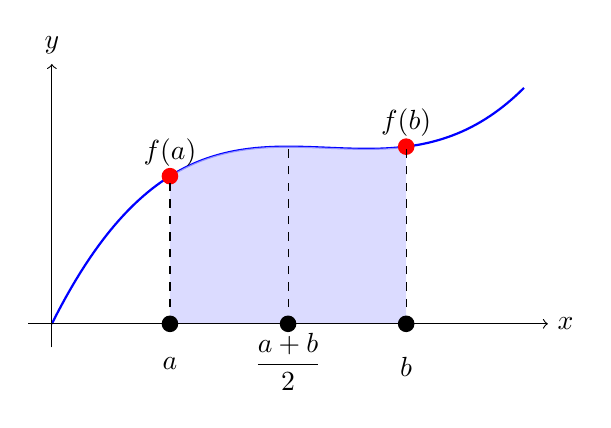
\begin{tikzpicture}[scale=3]
    % Define the function
    \def\f(#1){0.5*(#1)^3 - 1.75*(#1)^2 + 2*(#1)}

    % Define points
    \def\a{0.5}
    \def\b{1.5}
    \def\c{1}

    % Draw the function
    \draw[thick, blue, domain=0:2, samples=100] plot (\x, {\f(\x)});

    % Shade region between a and b
    \fill[blue!20, opacity=0.7] (\a,0) -- plot[domain=\a:\b, samples=50] (\x, {\f(\x)}) -- (\b,0) -- cycle;

    % Draw axes
    \draw[->] (-0.1,0) -- (2.1,0) node[right] {\(x\)};
    \draw[->] (0,-0.1) -- (0,1.1) node[above] {\(y\)};

    % Dots at the required points
    \foreach \x in {\a, \b, \c} {
        \fill (\x, 0) circle (1pt);
    }
    \foreach \x in {\a, \b} {
      \fill[red] (\x, {\f(\x)}) circle (1pt);
    }

    \draw[dashed] (\a,0) -- (\a, {\f(\a)});
    \draw[dashed] (\b,0) -- (\b, {\f(\b)});
    \draw[dashed] (\c,0) -- (\c, {\f(\c)});

    % Labels for the points
    \node[below] at (\a, -0.1) {\(a\)};
    \node[below] at (\b, -0.1) {\(b\)};
    \node[below] at (\c, 0) {$\displaystyle\frac{a+b}{2}$};
    \node[above] at (\a, {\f(\a)}) {\(f(a)\)};
    \node[above] at (\b, {\f(\b)}) {\(f(b)\)};
  \end{tikzpicture}
\end{center}
% The weighted mean value theorem can be applied to make integrating the error
% eassy.

If we use the usual strategy of integrating the error term for the Lagrange
polynomial then we get an $O(h^4)$ error. A sharper estimate can be obtained
using an alternative approach. 

Expand $f$ about $x$, using the third Taylor polynomial:

\begin{align*}
  f(x) &= f(x_1) + f'(x_1)(x - x_1) + \frac{f''(x_1)(x - x_1)^2}{2} \\
       &\quad+ \frac{f'''(x_1)(x - x_1)^3}{6} + \frac{f^{(4)}(\xi(x))(x -
       x_1)^4}{24}
\end{align*}

\begin{align*}
  \int_{x_0}^{x_2} P_3(f(x)) \, dx &= \left[ f(x_1)(x - x_1) + \frac{f'(x_1)}{2} (x - x_1)^2 + \frac{f''(x_1)}{6} (x - x_1)^3 \right. \\
                              &\quad \left. + \frac{f'''(x_1)}{24} (x - x_1)^4 \right]_{x_0}^{x_2} \\
                              &\quad + \frac{1}{24} \int_{x_0}^{x_2} f^{(4)}(\xi(x)) (x - x_1)^4 \, dx
\end{align*}

\begin{align*}
  \text{Consider} &\quad \frac{1}{24} \int_{x_0}^{x_2} f^{(4)}(\xi(x)) (x - x_1)^4 \, dx \\
                  &= \frac{f^{(4)}(\xi_1)}{24} \int_{x_0}^{x_2} (x - x_1)^4 \, dx \\
                  &= \frac{f^{(4)}(\xi_1)}{120} (x - x_1)^5 \Big|_{x_0}^{x_2} \\
                  &= \frac{f^{(4)}(\xi_1)}{60} h^5
\end{align*}

\[
  \therefore 
    \int_{x_0}^{x_2}f(x) \, dx = 2hf(x_1) + \frac{h^3}{3}f''(x_1) +
    \frac{f^{(4)}(\xi_1)h^5}{60}
.\]

But, we know that $\displaystyle f''(x_1) = \frac{1}{h^2} \left[ f(x_0) -2f(x_1) + f(x_2)
\right] + \frac{h^2}{12}f^{(4)}(\xi_1)$.

\begin{align*}
  \int_{x_0}^{x_2}f(x) \, dx &= 2hf(x_1) +
  \frac{h^3}{3}\left[\frac{1}{h^2}(f(x_0) - 2f(x_1) + f(x_2))
  -\frac{h^2 f^{(4)}(\xi_2)}{12} \right] \\
                             &\quad+ \frac{f^{(4)}(\xi_1)}{60}h^5\\
                             &= \frac{h}{3}\left[f(x_0)+4f(x_1)+f(x_2)\right]+O(h^5)
\end{align*}

This integration rule is known as \textbf{Simpson's Rule}:

\[
  \int_{x_0}^{x_2} f(x) \, dx = \frac{h}{3} \left[f(x_0)+4f(x_1)+f(x_2)\right] -
  \underbrace{\frac{h^5}{90}f^{(4)}(\xi)}_{\text{part of assignment 4}}
\]



\section*{Lecture Outline}

\begin{enumerate}
\item Starts with a review of the previous lecture, including:
  \begin{enumerate}[label=(\alph*)]
  \item Interpolation with two points (Trapezoidal Rule)
  \item Interpolation with three points (Simpson's Rule)
  \end{enumerate}
\item The \textbf{error analysis} of numerical integration methods.
  \textbf{(\ref{sec:error_analysis})}.
  \begin{enumerate}[label=(\alph*)]
  \item Simpson's Rule, despite using a quadratic approximation, can integrate
    up to a cubic. (Integrating a quadratic gives a cubic, and the method
    specifically finds a nice cancellation that allows higher order
    approximations)
  \item Definition of the degree of accuracy \ref{sec:degree_of_accuracy}
  \end{enumerate}
\item It turns out that Simpson's Rule and the Trapezoidal Rule are not the only
  methods of numerical integration. In fact, there are infinitely many methods
  of numerical Integration: The \textbf{Newton-Cotes Formulas
  (\ref{sec:newton_cotes_formulas})}.
  \begin{enumerate}[label=(\alph*)]
  \item Even-degree Newton-Cotes formulas are more accurate than odd.
  \item The formulas are \textbf{exact} if the degree of accuracy
    is greater than or equal to the degree of the function it is approximating.
  \item The Newton-Cotes formulas are \textbf{closed} if the endpoints of the
    interval are included as nodes. The formulas are \textbf{open
    (\ref{sec:open_newton_cotes_formulas})} if the nodes are all contained in
    the open interval $(a,b)$.
  \end{enumerate}
\item Finally, we discuss the \textbf{composite numerical integration
  (\ref{sec:composite_numerical_integration})} method. This method uses
  Newton-Cotes formulas to approximate the integral of a function over an
  interval.
\end{enumerate}

\section{Error Analysis of Numerical Integration Methods}
\label{sec:error_analysis}

\begin{center}
  \begin{tabular}{c|c|c}
    $f(x)$ & Simpson's & Trapezoidal \\ 
    \hline
    $x$ & 0 & 0 \\
    $x^3$ & nonzero & 0
  \end{tabular}
\end{center}

Simpson's Rule can integrate up to a cubic, even though the function used to
approximate the integral is a quadratic.  This is because in Simpson's Rule,
the quadratic approximation is integrated and there is a cancellation that
occurs, which allows the quadratic approximation to be used to approximate
the integral.

\subsection{Degree of Accuracy}
\label{sec:degree_of_accuracy}

\defn The \textbf{degree of accuracy} or precision of a quadratic formula is the largest
positive integer $n$ such that the formula is exact for $x^k$ when $k=0,1,\dots,n$.

\begin{center}
  \begin{tabular}{c|c}
    & Degree of Accuracy \\ \hline
    Trapezoid Rule & 1 \\
    Simpson's Rule & 3 \\
  \end{tabular}
\end{center}

\section{Newton-Cotes Formulas}
\label{sec:newton_cotes_formulas}

The Trapezoid and Simpson's Rules are examples of \textbf{Newton-Cotes
Formulas}. The $(n+1)$-point \uline{closed} Newton-Cotes formula uses nodes $x_i
= x_0+ih$ for $i=0,1,\dots,n$ where 

\begin{align*}
  x_0 &= a, \\
  x_n &= b, \\
  h &= \frac{b-a}{n}
\end{align*}

\noindent
Then,

\begin{align*}
  \int_{a}^{b} f(x) \, dx \approx \int_{a}^{b} P_n(x) \, dx 
  &= \int_{a}^{b} \sum_{i=0}^{n} h_i(x)f(x_i) \, dx \\
  &= \sum_{i = 0}^{n} \int_{a}^{b} L_i(x)f(x_i) \, dx \\
  &= \sum_{i = 0}^{n} a_i f(x_i)
\end{align*}

where $\displaystyle a_i = \int_{a}^{b} L_i(x) \, dx$

The formula is closed because the endpoints of the interval are included as
nodes. An error analysis of the Newton-Cotes formulas gives an interesting
result:

\thm Suppose that $\displaystyle \sum_{i = 0}^{n} a_if(x_i)$ denotes the $n+1$
point closed Newton-Cotes formula with $x_0=a, x_n=b$ and $h = \frac{b-a}{n}$.
If $n$ is even and $f\in C^{n+2}[a,b]$ then there exists $\xi \in (a,b)$ with 

\[
\int_{a}^{b} f(x) \, dx = \sum_{i = 0}^{n} a_if(x_i) +
\frac{h^{n+3}f^{(n+2)}(\xi)}{(n+2)!} \int_{0}^{n} t^2(t-1)\dots (t-n) \, dt
.\]

If $n$ is odd and $f\in C^{n+1}[a,b]$ then there exists $\xi \in (a,b)$ with

\[
  \int_{a}^{b} f(x) \, dx = \sum_{i = 0}^{n} a_if(x_i) +
  \frac{h^{n+2}f^{n+1}(\xi)}{(n+1)!} \int_{0}^{n} t(t-1)\dots(t-n) \, dt
.\]

Notice that the degree of precision is $n+1$ and the error is $O(h^{n+3})$ if
$n$ is even. If $n$ is odd then the degree of precision is only $n$ and hte
error is only $O(h^{n+2})$.

\begin{center}
  \begin{tabular}{c|l c}
    $n$ & \textbf{Name} & \textbf{Error Term} \\
    \hline
    1 & Trapezoid Rule & $-\frac{h^3}{12} f''(\xi)$ \\
    2 & Simpson's Rule & $-\frac{h^5}{90} f^{(4)}(\xi)$ \\
    3 & Simpson's Three-Eighths Rule & $-\frac{3h^5}{80} f^{(4)}(\xi)$ \\
    4 & & $-\frac{h^7}{945} f^{(6)}(\xi)$ \\
  \end{tabular}
\end{center}

\subsection{Open Newton-Cotes Formulas}
\label{sec:open_newton_cotes_formulas}
There are also \uline{open} Newton-Cotes formulas. here,

\begin{align*}
x_i &= x_0+ih \qquad i = 0,1,\dots,n \\
x_0 &= a+h \\
h = \frac{b-a}{n+2}
\end{align*}

Then the open Newton-Cotes formulas are given by

\begin{equation}
  \int_{a}^{b} f(x) \, dx \approx \sum_{i = 0}^{n} a_if(x_i) 
.\end{equation}

where $\displaystyle a_i = \int_{a}^{b} L_i(x) \, dx$

Note that $x_0 = a+h$ and $x_n = b-h$. The formulas are \uline{open} because the
nodes are all contained in the open interval $(a,b)$. Once again, if $n$ is even,
the degree of precision is $(n+1)$ and the error is $O(h^{n+3})$. If $n$ is odd,
the degree of precision is only $n$ and the error is only $O(h^{n+2})$.

Some examples of open Newton-Cotes formulas are:

\begin{tabular}{c| l}
    $n$ & \\
    \hline
    0 & $\displaystyle 2h f(x_0) + \frac{h^3}{3} f''(\xi), \quad \text{where } \xi \in (a,b)$ \\[10pt]
    1 & $\displaystyle \frac{3h}{2} \left[ f(x_0) + f(x_1) \right] + \frac{3h^3}{4} f''(\xi), \quad \text{where } \xi \in (a,b)$ \\[10pt]
    2 & $\displaystyle \frac{4h}{3} \left[ 2f(x_0) - f(x_1) + 2f(x_2) \right] + \frac{14h^5}{45} f^{(4)}(\xi)$ \\[10pt]
    3 & $\displaystyle \frac{5h}{24} \left[ 11f(x_0) + f(x_1) + f(x_2) + 11f(x_3) \right] + \frac{95}{144} h^5 f^{(4)}(\xi)$ \\
\end{tabular}

$n=0$ is also called the \textbf{Midpoint Rule}. 

\section{Composite Numerical Integration}
\label{sec:composite_numerical_integration}
Typically, we do not apply Newton-Cotes formulas directly onto the interval
$[a,b]$. If we did, then high degree formulas would be required to obtain
accurate solutions, but as we have already seen, these high degree polynomials
would give an oscillatory and innacurate interpolation. To avoid this problem,
we prefer a piecewise approach to numerical integration that uses low order
Newton-Cotes formulas.

\Ex Simpson's Rule

\begin{center}
  \begin{tikzpicture}[scale=2.0]
    % Draw axes
    \draw[->] (-0.1,0) -- (6.5,0) node[below] {$x$};
    \draw[->] (0,-0.1) -- (0,2.2) node[left] {$y$};

    % Define function
    \draw[thick, red, domain=0:6, samples=100] 
      plot(\x, {0.05375*\x*\x*\x - 0.520625*\x*\x + 1.4803125*\x});

    % Draw dotted vertical lines
    \foreach \x in {0.5,1,1.5,2,2.5,4.5,5,5.5} {
      \draw[thick, dotted, blue] (\x,0) -- (\x,{0.05375*\x*\x*\x - 0.520625*\x*\x + 1.4803125*\x});
    }

    \foreach \x in {0.5, 1.5, 2.5, 4.5, 5.5} {
      \draw[thick, blue] (\x,0) -- (\x,{0.05375*\x*\x*\x - 0.520625*\x*\x + 1.4803125*\x});
      % \node[below] at (\x,-0.05) {$x_{\x}$};
    }

    % \node at (3.5, 0.5) {$\LARGE{\dots}$};
    \foreach \i in {0,1,2} {
        \fill (3.3 + \i*0.2, 0.5) circle (1.0pt);
    }

    \node[below] at (0.5, -0.05) {$x_0$};
    \node[below] at (1.5, -0.05) {$x_2$};
    \node[below] at (2.5, -0.05) {$x_4$};
    \node[below] at (4.5, -0.05) {$x_{n-2}$};
    \node[below] at (5.5, -0.05) {$b=x_n$};

  \end{tikzpicture}
\end{center}

% image goes here

We divide the interval into an even number of subintervals. Simpson's rule is
applied on each consecutive pair of subintervals.

\[
  \frac{h}{3} \left[f(x_i) + 4f(\frac{x_i+x_{i+2}}{2}) + f(x_{i+2})\right]
.\]

Take $\displaystyle h=\frac{(b-1)}{n}$ and $x_j = a + jh$. Then,

\begin{align*}
  \int_{a}^{b} f(x) \, dx &= \sum_{j=1}^{\frac{n}{2}} \int_{x_{2j-2}}^{x_{2j}}
  f(x) \, dx \\
                          &= \sum_{j=1}^{\frac{n}{2}} \left\{
                            \frac{h}{3} \left[
                              f(x_{2j-2}) + 4f(x_{2j-1}) + f(x_{2j})
                            \right] - \frac{h^5}{90} f^{(4)}(\xi_j)
                          \right\} \\
                          &\qquad\text{where } x_{2j-2} < \xi_j < x_{2j} \\
                          &\qquad\text{and } f \in C^4[a,b]
\end{align*}

taking into account that $f(x_{2j}), 0 < j < \frac{n}{2}$ appears in 2 terms,
this summation can be simplified somewhat

\[
  \int_{a}^{b} f(x) \, dx = \frac{h}{3} \left[
    f(x_0) + 2 \sum_{j=1}^{\frac{n}{2}-1} f(x_{2j}) + 4 \sum_{j=1}^{\frac{n}{2}}
    f(x_{2j-1}) + f(x_n)
  \right] + \text{error}
.\]


got to page 41/80 (32/54 in the published lecture slides)

\section*{Lecture Outline}
\begin{enumerate}
\item 
\end{enumerate}

\section{Error Behavior of Simpson's Rule (19.12)}

It is important to understand the stability property of \textbf{Composite
Newton-Cotes} integration techniques.

Assume $f(x_i)$ is approximated by $\tilde{f}(x_i)$:

\begin{equation*}
  f(x_i) = \tilde{f} (x_i) + e_i \qquad 0 \leq i \leq n
.\end{equation*}

\noindent
where $e_i$ is the roundoff associated with using $\tilde{f}$ to approximate
$f$. Then, the accumulated roundoff error in the Composite Simpson's Rule is

\begin{align*}
  |e(h)| &= \left|\frac{h}{3} \left[
    e_0 + 2 \sum_{j=1}^{\frac{n}{2}-1} e_{2j} + 4 \sum_{j=1}^{\frac{n}{2}}
    e_{2j-1} + e_n
  \right]\right| \\
         & \leq \frac{h}{3} \left[
           |e_0| + 2 \sum_{j=1}^{\frac{n}{2}-1} |e_{2j}| + 4 \sum_{j=1}^{\frac{n}{2}}
           |e_{2j-1}| + |e_n|
         \right]
\end{align*}

We have a triangle inequality. Assume all $e_j$ are bounded by $\bigEps$.

\begin{equation*}
  h = \frac{(b-a)}{n}
\end{equation*}


\begin{align*}
  |e(h)| & \leq \frac{h}{3} \left[
    \bigEps + 2(\frac{n}{2} -1)\bigEps + 4 \frac{n}{2} \bigEps + \bigEps
  \right] \\
         &= \frac{h}{3} 3n \bigEps \\
         &= nh \bigEps \\
         &= (b-a) \bigEps \\
\end{align*}

Which is indepentent of $h$ which implies the procedure is stable as $h\to 0$

\section{Romberg Integration}
\label{sec:romberg_integration}
An interesting point concerning the composite Trapezoid Rule:

If $f= \in C^2[a,b]$ then there exists a $\mu \in [a,b]$ such that 

\begin{align*}
  \int_{a}^{b} f(x) \, dx &= \frac{h}{2} \left[
    f(a) + 2 \sum_{j=1}^{h-1} f(x_j) + f(b)
  \right] - \frac{b-a}{12}h^2 f''(\mu) \\
                          &\text{where } h = \frac{b-1}{n} \\
                          &\text{and } x_j = a + jh
\end{align*}

Thus the error for the composite Trapezoid Rule is $O(h^2)$. In fact we can be
more precise. An application of the Euler-MacLaurin summation formula shows that
for sufficiently smooth $f$,

\begin{align*}
  \text{error} \quad&\quad= c_1 h^2 + c_2 h^4 + \dots + c_m h^{2m} + O(h^{2m+2}) \\
  \text{where}\quad &c_k = \text{const} \times \left(
    f^{(2k-1)}(b) - f^{(2k-1)}(a)
  \right)
\end{align*}

This shows us that the Composite Trapezoid Rule is extremely accurate for smooth
periodic functions, provided $h$ is small enough.

*Note: The error expansion contains only even powers of $h$, so eliminating the 
leading error term improves the accuracy by two additional orders of $h$.

Notice that we know the form of the error, so we can obtain higher order
accuracy by using Richardson Extrapolation. (To give Romberg Integration)

\subsection{Richardson Extrapolation to obtain Romberg Integration}
\label{sec:richardson_extrapolation_to_obtain_romberg_integration}

We will carry out Composite Trapezoid Rule approximations with 

\[
  m_1 = 1, m_2 = 2, m_3 = 4, \dots, m_n = 2^{n-1} \text{ intervals.} 
.\]

The values of the step sizes $h_k$ corresponding to $m_k$ are 

\[
  h_k = \frac{(b-1)}{m_k} = \frac{(b-1)}{2^{k-1}}
.\]

With this notation, the Composite Trapezoid Rule becomes

\begin{equation*}
  \int_{a}^{b} f(x) \, dx = \frac{h_k}{2} \left[
    f(a) + 2\left(
      \sum_{i=1}^{2^{k-1}-1} f(a+ih_k) 
      \right)
      - \frac{(b-a)}{12} h^2_k f''(\mu_k)
  \right]
.\end{equation*}

where $\mu_k \in (a,b)$

Let $R_{k,1}$ be the approximation to the integral using $m_k=2^{k-1}$
intervals.

\ie 

\begin{align*}
  R_{1,1} &=  \frac{h_1}{2}\left[
    f(a)+f(b)
  \right] = \frac{(b-1)}{2}
  \left[
    f(a)+f(b)
  \right]
\end{align*}

\begin{align*}
  R_{2,1} &= \frac{h_2}{2} \left[
    f(a)+f(b)+2f(a+h_2)
  \right] \\
          &= \frac{(b-a)}{4} \left[
            f(a)+f(b)+2f(a+\frac{b-1}{2})
          \right] \\
          &= \frac{1}{2} \left[
            R_{1,1} + h_1f(a+h_2)
          \right]
\end{align*}

notice that when $h$ is halved, all the old points at which the function was
evaluated appear in the new computation- we can avoid repeating the evaluations.

\begin{equation*}
  R_{3,1} = \frac{1}{2} \left\{
    R_{2,1} + h_2 \left[
      f(a+h_3) + f(a+3h_3)
    \right]
  \right\}
.\end{equation*} 

\[
\vdots
\]

\begin{equation*}
  R_{k,1} = \frac{1}{2} \left\{
    R_{k-1,1} + h_{k-1} \left[
      \sum_{i=1}^{2^{k-2}} f(a+(2i-1)h_k)
    \right]
  \right\}
.\end{equation*}

We can apply this equation to perform the first step of Romberg Integration for

\begin{equation*}
  \int_{0}^{1} e^{-x} \, dx = 1-e^{-1} \approx 0.63212
.\end{equation*}

\begin{align*}
R_{1,1} &= \frac{(1-0)}{2} [e^{-0} + e^{-1}] \approx 0.68394 \\
R_{2,1} &= \frac{1}{2}\left[R_{1,1} + \frac{(1-0)}{2}e^{-(0+\frac{1}{2})}
\right] = 0.64523 \\
R_{3,1} &= 0.65341 \\
R_{4,1} &= 0.63294 \\
\end{align*}

We can obtain a faster convergence using Richardson Extrapolation:

Notice that:

\begin{align*}
\int_a^b f(x)\,dx - R_{h,1} 
&= \sum_{i=1}^{m} c_i h^{{2i}} + O(h^{2m+2}) \\
&= c_1 h^2 + \sum_{i=2}^{m} c_i h^{2i} + O(h^{2m+2})
\end{align*}

\begin{align*}
\int_a^b f(x)\,dx - R_{h/2,1} 
&= \sum_{i=1}^{m} c_i h_{h/2}^{2i} + O(h^{2m+2}) \\
&= \frac{c_1 h^2}{4} + \sum_{i=2}^{m} \left(\frac{c_i h^{2i}}{4^i}\right) + O(h^{2m+2})
\end{align*}

Subtracting the first from 4 times the second gives an $O(h_k^4)$ formula:

\begin{align*}
  \int_a^b f(x)\,dx - R_{h,2} 
&= \sum_{i=2}^{m} \frac{c_i}{3} \left( \left( \frac{h^{{2i}}}{4^i} \right) -
h^{2i} \right) + O(h^{2m+2}) \\
  \text{where} \quad R_{h,2} &= \frac{R_{h,1} + R_{h/2,1} - R_{h,1}}{3}
\end{align*}

Of course, this procedure can be repeated to eliminate the $O(h_k^4)$ term from
the error. Continuing in this manner, we have an $O(h_k^{2j})$ approximation
formula defined by 

\begin{equation*}
  R_{kj} = R_{k, j-1} + \frac{R_{k,j-1} - R_{k-1, j-1}}{4^{j-1}-1}
.\end{equation*}

\Ex Use Romberg Integration to approximate 

\[
  \int_{0}^{1} e^{-x} \, dx
.\]

to $5$ significant digits.

\begin{tabular}{c|ccccc}
      & $R_{h,1}$ & $R_{h,2}$ & $R_{h,3}$ & $R_{h,4}$ & $R_{h,5}$ \\
\hline
  $R_{1,j}$ & .6839397 &          &          &        &            \\
  $R_{2,j}$ & .6452352 & .6723337 &          &        &            \\
  $R_{3,j}$ & .6354094 & .6321312 & .6321209 &        &            \\
  $R_{4,j}$ & .6329434 & .6321214 & .6321206 & .6321206 &          \\
  $R_{5,j}$ & .6323263 & .6321206 & .6321206 & .6321206 & .6321206 \\
\end{tabular}

A typical stopping criterion is that both

\[
  |R_{n-1, n-1} - R_{n,n} \text{ and } |R_{n-2,n-2} - R_{n,n}| < \bigEps
.\]

for some error tolerance $\bigEps$.

Note that we may not observe the expected convergence acceleration if

\begin{itemize}
  \item The integrand $f$ is not sufficiently smooth. We need $f\in
    C^{2k+2}[a,b]$ to generate the $k^{th}$ row of the table.
  \item The coefficients $c_1, c_2, \dots$ are very small. This happens for
    periodic functions if the interval of integration is an integer multiple of
    the period or for functions with extremely small derivatives at the
    endpoints of the interval of integration.
\end{itemize}

\section{Adaptive Quadrature}

Composative quadrature rules necessitate the use of equally spaced points. This
does not take into account that some portions of the curve may have large
functional variations that require more attention than other portions of the
curve. It is useful to introduce a method that adjusts the step size to be
smaller over portions of the curve where a larger functional variation occurs.
Thi technique is called adaptive quadrature. We will now discuss an adaptive
based on Simpson's Rule. The other composite procedures can be modified in a
similar manner.


\section{Adaptive Quadrature}
\label{sec:adaptive_quadrature}

Composative quadrature rules necessitate the use of equally spaced points. This
does not take into account that some portions of the curve may have large
functional variations that require more attention than other portions of the
curve. It is useful to introduce a method that adjusts the step size to be
smaller over portions of the curve where a larger functional variation occurs.
Thi technique is called adaptive quadrature. We will now discuss an adaptive
based on Simpson's Rule. The other composite procedures can be modified in a
similar manner.

We want to approximate 

\begin{equation*}
  \int_{a}^{b} f(x) \, dx
\end{equation*}

to within a specified tolerance $\bigEps > 0$.

We will start by applying Simpson's Rule with a step size $h=\frac{(b-a)}{2}$

\begin{align*}
  \int_{a}^{b} f(x) \, dx &= S(a,b) - \frac{h^5}{90}f^{(4)} (\mu)\\
  \text{where} \quad  S(a,b) &= \frac{h}{3}\left[f(a) + 4f(a+h) +f(b)\right]
  \qquad (*)\\
    \text{and} \quad  \mu &\in (a,b)
.\end{align*}

We want to know if we should further subdivide the interval, so we need an
estimate for the error. Unfortunately, we don't know $f^{(4)}(\mu)$. Instead, we
will estimate the error using Simpson's Rule with a step size $\frac{(b-a)}{4}$

\begin{align*}
  \int_{a}^{b} f(x) \, dx &= \frac{h}{6} \left[
    f(a) + 4f(a+\frac{h}{2}) + 2f(a+h) +4f(a+ \frac{3h}{2}) + f(b)
  \right] \\
                          &- (\frac{h}{2})^4 \frac{(b-a)}{180} f^{(4)} (\tilde{\mu})
.\end{align*}

for some $\tilde{\mu} \in (a,b)$.

\uline{OR}

\begin{align*}
  \int_{a}^{b} f(x) \, dx &= S(a, \frac{(a+b)}{2}) + S(\frac{(a+b)}{2}, b) -
  \frac{1}{16} \frac{h^5}{90} f^{(4)} (\tilde\mu) \\
  \text{where} \quad  S(a, \frac{(a+b)}{2}) &= \frac{h}{6} \left[
    f(a) + 4f(a+\frac{h}{2}) + f(a+h)
  \right] \qquad (**)\\
    \text{and} \quad  S(\frac{(a+b)}{2},b) &= \frac{h}{6} \left[
      f(a+h) + 4f(a+\frac{3h}{2}) + f(b)
      \right]
\end{align*}

Now, we assume $f^{(4)}(\mu) \approx f^{(4)}(\tilde\mu)$.

\noindent
\uline{Note:} if $f^{(4)}$ is continuous, this assumption will hold for
sufficiently small $h$.

Subtract (**) from (*) to obtain

\[
0 \equiv S(a,b) - S\left(a, \frac{a+b}{2}\right) - S\left(\frac{a+b}{2}, b\right) - \frac{15}{16} \cdot \frac{h^5}{90} f^{(4)}(\mu)
\]
\[
\text{or} \frac{h^5}{90} f^{(4)}(\mu) \approx \frac{16}{15} \left[ \mathcal{I}(a,b) - \mathcal{I}\left(a, \frac{a+b}{2}\right) - \mathcal{I}\left(\frac{a+b}{2}, b\right) \right]
.\]

\begin{align*}
\therefore \quad \left| \text{error} \right| 
&= \left| \int_a^b f(x) \, dx - \mathcal{I}\left(a, \frac{a+b}{2}\right) - \mathcal{I}\left(\frac{a+b}{2}, b\right) \right| \\
&\equiv \frac{1}{16} \left| \frac{h^5}{90} f^{(4)}(\mu) \right| \\
&\equiv \frac{1}{15} \left| \mathcal{I}(a,b) - \mathcal{I}\left(a, \frac{a+b}{2}\right) - \mathcal{I}\left(\frac{a+b}{2}, b\right) \right|
\end{align*}

Thus if we want $|\text{error}|<\bigEps $, we typically insist that 

\[
\frac{1}{10} |S(a,b)-S(a,\frac{a+b}{2}) - S(\frac{a+b}{2}, b)| \leq \bigEps
.\]

Often, a factor of $\frac{1}{10}$ is used rather than $\frac{1}{15}$ since we
had to make the assumption that $f^{(4)}(\mu) \approx f^{(4)}(\tilde\mu)$ and we
prefer to be somewhat conservative in our error estimates.

From last day, we had an error estimate for Simpson's Rule: 

\[
E = \frac{1}{15} |S(a,b)-S(a,\frac{a+b}{2}) - S(\frac{a+b}{2}, b)|
.\]

\Ex Compute the Simpson's Rule approximations for

\[
\int_{a}^{1.5} x^2 \ln(x) \, dx = 0.19225935
.\]

and calculate the error estimate and the actual error.

In deriving our eror estimate, we had to make the assumption that $f^{(4)}(\mu)
\approx f^{(4)}(\tilde\mu)$, and to compensate for this error we typically
insist that

\[
\frac{1}{15} |S(a,b)-S(a,\frac{a+b}{2}) - S(\frac{a+b}{2}, b)| < \frac{2}{3}
\bigEps \equiv \tilde\bigEps
.\]

Adaptive quadrature methods are built on top of this condition. If the error
estimate is less than $\frac{2}{3}$ the desired tolerance $\bigEps$, then 

\[
S(a, \frac{(a+b)}{2}) + S(\frac{(a+b)}{2}, b)
.\]

is assumed to be a sufficiently accurate approximation to $\int_{a}^{b} f(x) \, dx$ 

Otherwise, we apply Simpson's Rule to the subintervals $[a, \frac{a+b}{2}]$ and
$[\frac{a+b}{2}, b]$. We also use the error estimation in each of the
subintervals. If each error estimate is less than $\frac{\bigEps}{2}$, then we
sum the approximations to get an approximation of $\int_{a}^{b} f(x) \, dx$.

If the approximation on one of the subintervals fails to be within the tolerance
$\frac{\tilde \bigEps}{2}$ then that subinterval is itself subdivided and the
procedure is reapplied to the two subintervals to determine if the approximation
on each subinterval is accurate to within $\frac{\tilde \bigEps}{2}$.

This recursive procedure is continued until each portion is within the desired
tolerance.

\section{Gaussian Quadrature}

Thus far we hvae onlyd ealt with quadrature formulae

\[
\int_{a}^{b} f(x) \, dx \approx \sum_{j=1}^{n} a_j f(x_j)
.\]

that relied on nodes that are equally spaced. This is a nice feature for
composite rules because it reduces the number of function evaluations. However,
if we allow ourselves to use unequally spaced points, then we can construct
quadrature formulas of higher order accuracy.

Notice that with $n$ nodes and $n$ weights we have $2n$ free parameters and we
may hope to find an optimal quadrature formula which is exact for polynomials of
degree $\leq 2n-1$.

First, note that an integral

\[
\int_{a}^{b} f(x) \, dx
.\]

over an interval $[a,b]$ can be transformed into an integral over $[-1, 1]$ by
using a change of variables

\begin{align*}
\text{let}\quad t &= \frac{2x-a-b}{b-a} \\
\text{then}\quad  x &= \frac{1}{2}[(b-a) + a + b] \\
\text{and} \quad \,dx &= \frac{1}{2}(b-a) \,dt
\end{align*}

So 

\[
  \int_{a}^{b} f(x) \, dx = \int_{-1}^{1} f(\frac{1}{2}[(b-a)t + a+b]) \,
  \frac{1}{2}(b-a)dt
.\]

so without loss of generality, we will consider integrals over the interval $[-1,1]$.

Suppose that $n=2$ (2 nodes) and that we want to determine $c_1, c_2, x_1, x_2$
so that the integration formula

\[
\int_{-1}^{1} f(x) \, dx = c_1 f(x_1) + c_2 f(x_2)
.\]

gives the exact result whenever $f(x)$ is a polynomial of degree $2(2)-1 =3$.

\[
\ie f(x) = a_0 + a_1 x + a_2 x^2 + a_3 x^3
.\]

Since 

\begin{align*}
&\int_{-1}^{1} a_0 + a_1 x + a_2 x^2 + a_3x^3 \, dx  \\
&= a_0 \int_{-1}^{1}  \, da + a_1 \int_{-1}^{1} x \, dx + a_2 \int_{-1}^{1} x^2 \, dx + a_3 \int_{-1}^{1} x^3 \, dx \\
\end{align*}

This problem is equivalent to showing that the formula is exact for $f(x) = 1,
x, x^2, x^3$.

cases:

\begin{center}
  \begin{tabular}{c|c}
    Function $f(x)$ & Equation \\
    \hline
    $1$ & $c_1 + c_2 = a_0 \int_{-1}^{1} \, dx$ \\
    $x$ & $c_1x_1 + c_2x_2 = \int_{-1}^{1} x \, dx$ \\
    $x^2$ & $c_1x_1^2 + c_2x_2^2 = \int_{-1}^{1} x^2 \, dx$ \\
    $x^3$ & $c_1x_1^3 + c_2x_2^3 = \int_{-1}^{1} x^3 \, dx$ \\
  \end{tabular}
\end{center}

Solving this system gives us that

\[
c_1 = 1, c_2 = 1, x_1 = - \frac{\sqrt{3}}{3}, x_2 = \frac{\sqrt{3}}{3}
.\]

$\implies$ the approximation formula is 
\[
  \int_{-1}^{1} f(x) \, dx = f\left(-\frac{\sqrt{3}}{3}\right) +
  f\left(\frac{\sqrt{3}}{3}\right)
.\]

This approach can be used to obtain the nodes and coefficients for larger $n$,
but Legendre polynomials can be used to obtain them more easily.

\subsection{Legendre Polynomials}

The Legendre Polynomials are defined according to the following two properties:

\begin{enumerate}
\item $P_n(x)$ is a polynomial of degree $n$
\item $\int_{-1}^{1} P(x)P_n(x) \, dx = 0$ whenever $P(x)$ is a polynomial of
  degree less than $n$.
\end{enumerate}


\section{Initial Value Problems for ordinary Differential Equations}

Many natural, scientific and engineering problems can be described in terms of 
\uline{differential equations}. Differential equations give us a way to
mathematically expres rates of change. We will be considering methods for
treating ordinary differential equations (ODEs) in this lecture. ODEs only
consider derivatives with respect to one variable.

\Ex Let $y(t)$ denote the number of individuals in a certain population. If this
population has a constant growth rate $\alpha$ (the difference between a
constant birth rate and death rate), then the differential equation 

\[
y'(t) = \alpha y(t)
.\]

with initial condition $y(0) = y_0$ describes the population growth.

\soln 

% \begin{align*}
%   \frac{y'}{y} &= \alpha \\
%   \frac{dy}{y} &= \alpha \, dx \\
%   \int \frac{dy}{y} &= \int \alpha \, dx \\
%   \ln |y| &= \alpha x + C \\
%   |y| &= e^{\alpha x + C} = e^C \cdot e^{\alpha x} \\
%   y &= C_1 e^{\alpha x} \quad \text{where } C_1 = \pm e^C
% \end{align*}

\begin{align*}
  \frac{y'(t)}{y(t)} &= \alpha \\
  D_t[\ln(y(t))] &= \alpha \\
  \ln(y(t)) &= \alpha t + \text{const}  \\
  y(t) &= ce^{\alpha t} \qquad c = e^{\text{const}}\\
\end{align*}

\begin{equation*}
  y(0) = y_0 \implies y(t) = y_0 e^{\alpha t}
.\end{equation*}

To include other effects such as overcrowding, competition for food, etc, one
might introduce a second term into the equation

\begin{equation*}
  y'(t) = \alpha y(t) - \beta [y(t)]^2
.\end{equation*}

where $\beta > 0$ and $\beta$ is small. Introducing a nonlinear term makes the
problem much more difficult to study analytically.

Indeed, few problems originating from the study of physical phenomena can be
solved exactly. We begin by studying numerical methods for approximating the
solution $y(t)$ to a problem.

\[
  \frac{dy}{dt} = f(t, y) \qquad \text{for } a \leq t \leq b
.\]

subject to the initial condition 

\[
y(a) = \alpha
.\]

\subsection{The elementary theory of initial value problems}

We want/need some theoretical results, in particular, we would like to show that
solutions to equations exist and are unique.

\defn A function $f(t,y)$ satisfies a Lipschitz condition in the variable $y$ on
a set $D \in \mathbb{R}^2$ if a constant $L > 0$ exists such that

\[
  |f(t,y_1) - f(t, y_2)| \leq L|y_1 - y_2| \qquad \text{for all } (t,y_1), (t,y_2) \in D
.\]

The constant $L$ is called a \uline{Lipschitz constant} for $f$.

\pagebreak
\subsubsection{Example}

Does $f(t,y) = ty$ satisfy a Lipschitz condition on 

\[
D  = \{(t,y) : 0 \leq t \leq 1, -\infty < y < \infty\}
?\]

\noindent
\soln

% \begin{align*}
% &|f(t,y_1) - f(t, y_2)| \\
% &= |-ty_1 + \frac{4t}{y_1} + ty_2 - \frac{4t}{y_2}|\\
% \end{align*}

\begin{equation*}
|f(t,y_1) - f(t, y_2)| = |-ty_1 + \frac{4t}{y_1} + ty_2 - \frac{4t}{y_2}|
.\end{equation*}


Consider $y_1 = -1, t=1$, $y_2 \to 0^+$. Under these conditions, we have
$|f(t,y_1) - f(t,y_2)| \to \infty$.

RHS = $L|y_1-y_2| \to L$

$L$ is finite.

We cannot have $|f(t,y_1) - f(t,y_2)| \leq L|y_1 - y_2|$ for any finite $L$

$\therefore$ Lipschitz condition does not hold.


IDK why but he starts off with this example

\section{Quadrature Formula Example}

Find the constants $c_0, c_i$ and $x$ such that the quadrature formula

\begin{equation*}
  \int_{-1}^{0} f(x) \, dx = c_0 f(-1) + c_i f(x_1)
.\end{equation*}

has the highest degree of precision possible.

\uline{ans.}
 
\renewcommand{\arraystretch}{3}
\begin{center}
  \begin{tabular}{c|c}
    Function $f$ & Equation \\
    \hline
    $f(x) = 1$ & $\displaystyle \int_{-1}^{0} 1 \, dx = c_0 + c_i$ \\
    $f(x) = x$ & $\displaystyle \int_{-1}^{0} x \, dx = \left. \frac{x^2}{2} \right|_{-1}^0 = c_0 (-1) + c_i x_1 = -\frac{1}{2}$ \\
    $f(x) = x^2$ & $\displaystyle \int_{-1}^{0} x^2 \, dx = c_0 + c_i x_1^2 = \frac{1}{3}$ \\
  \end{tabular}
\end{center}

Next, we do some substutitions:

\begin{enumerate}
\item substitute (1) into (2) to eliminate $c_0$
\item substitute (1) into (3) to eliminate $c_0$
\end{enumerate}

We now have $2$ equations for $c_i + x_1$.

Solve: $c_0 = \frac{1}{4}, c_i = \frac{3}{4}, x_i = -\frac{1}{3}$

Could it be exact for cubics?

LHS = $\int_{-1}^{0} x^3 \, dx = -\frac{1}{4}$

RHS = $-\underbrace{c_0}_{\frac{1}{4}} +
\underbrace{c_i}_{\frac{3}{4}}\underbrace{x_i}_{-\frac{1}{3}}^3 \neq \text{LHS} $

So, no, it cannot be exact for cubics.

\section{Legendre Polynomials}

This approach can be used to obtain the nodes and coefficients for larger $n$,
but Legendre polynomials can be used to obtain them more easily.

The Legendre Polynomials are defined according to the following two properties:

\begin{enumerate}
\item $P_n(x)$ is a polynomial of degree $n$.\\
  $\implies P_0(x) = 1$ 
\item $\int_{-1}^{1} P(x)P_n(x) \, dx = 0$ whenever $P(x)$ is a polynomial of
  degree less than $n$.
\end{enumerate}

The first few Legendre polynomials are

\renewcommand{\arraystretch}{1.25}
\begin{center}
  \begin{tabular}{c|c}
    $P_n(x)$ & \\ \hline
    $P_0(x)$ & $1$ \\
    $P_1(x)$ & $x$ \\
    $P_2(x)$ & $x^2-\frac{1}{3}$ \\
    $P_3(x)$ & $x^3-\frac{3}{5}x$ \\
    $P_4(x)$ & $x^4-\frac{6}{7}x^2+\frac{3}{35}$ \\
  \end{tabular}
\end{center}

Some properties:

\begin{itemize}
\item The roots of these polynomials are distinct
\item The roots of these polynomials lie in $(-1, 1)$
\item The $P_n$'s are symmetrical about the origin\\
  $\implies$ the roots are symmetrical about the origin
\item The roots of the $n^{th}$ degree Legendre polynomial have the property
  that they are the nodes needed to produce an integral approximation formula
  that gives the exact result for any polynomial of degree less than $2n$.
\end{itemize}

\thm Suppose $x_1, x_2, \dots, x_n$ are the roots of the $n^{th}$ degree
Legendre polynomial $P_n(x)$ and that for each $i=1, 2, \dots, n$ the numbers
$c_i$ are defined by

\begin{equation*}
  c_i = \int_{-1}^{1} \prod_{\substack{j = 1 \\ j \ne i}}^{n} \frac{x-x_j}{x_i-x_j} \, dx
.\end{equation*}

If $P(x)$ is any polynomial of degree less than $2n$ then

\begin{equation*}
  \int_{-1}^{1} P(x) \, dx = \sum_{i=1}^{n} c_i P(x_i)
.\end{equation*}


\section{A continuation on the Elementary Theory of Initial Value Problems}

\subsection{Lipschitz Conditions}

\defn A function $f(t,y)$ satisfies a Lipschitz condition in the variable $y$ on
a set $D \in \mathbb{R}^2$ if a constant $L > 0$ exists such that

\[
  |f(t,y_1) - f(t, y_2)| \leq L|y_1 - y_2| \qquad \text{for all } (t,y_1), (t,y_2) \in D
.\]

The constant $L$ is called a \uline{Lipschitz Constant} for $f$.

*Examples can be found in the lecture notes for Lecture 31-b.*

\subsection{Convex Sets}

\defn A set $D\in \mathbb{R}^2$ is said to be \uline{convex} if whenever $(t_1,
y_1)$ and $(t_2,y_2)$ belong to $D$, the point
\begin{equation*}
  ((1-\lambda)t_1 + \lambda t_2, (1-\lambda)y_1 + \lambda y_2)
.\end{equation*}

\noindent
also belongs to $D$ for each $\lambda\in[0,1]$. Geometrically, a set is convex
if, for any two points in the set, a line segment connecting them lies entirely
within the set. (\ie every point in the set has line of sight to every other
point within the set.)

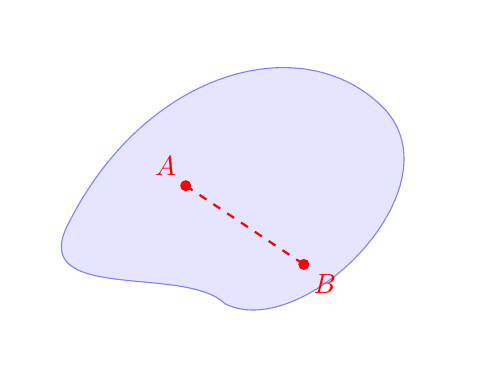
\begin{tikzpicture}

  % Draw the convex set as a smooth closed shape
  \filldraw[fill=blue!10, draw=blue!50] 
    (0,0) .. controls (1,2) and (3,2.5) .. (4,1.5)
    .. controls (5,0.5) and (3,-1.5) .. (2,-1)
    .. controls (1.5,-0.5) and (-0.5,-1) .. (0,0);

  % Two arbitrary points inside the convex set
  \fill[red] (1.5,0.5) circle (2pt) node[above left] {$A$};
  \fill[red] (3,-0.5) circle (2pt) node[below right] {$B$};

  % Line segment connecting the two points
  \draw[thick, red, dashed] (1.5,0.5) -- (3,-0.5);

\end{tikzpicture}

\subsubsection{Exercise 1 (22.5)}

Show that the set
\begin{equation*}
  D = \{(t,y):a\leq t\leq b, -\infty < y < \infty\}
.\end{equation*}
where $a$ and $b$ are constants, is convex.

To prove analytically, we can use the definition of convexity and show that each
point falls within the set.

\subsection{Theorem 1 (22.6)}

Suppose $f(t,y)$ is defined on a convex set $D\in \mathbb{R}^2$. If a constant
$L>0$ exists with
\begin{equation*}
  \abs{\frac{\partial f}{\partial y}(t,y)} \leq L
\end{equation*}

\noindent
then for all $(t,y) \in D$ then $f$ satisfies a Lipschitz condition on $D$ in
the variable $y$ with Lipschitz constant $L$.

\proof Let $(t, y_1)$ and $(t, y_2)$ be in $D$. Holding $t$ fixed, define 
$g(y) = f(t, y)$.

Suppose $y_1 \leq y_2$. Since the line joining $(t, y_1)$ to $(t, y_2)$ lies in
$D$ and $f$ is continuous on $D$ we have $g \in C[y_1, y_2]$. Furthermore,
\[
g'(y) = \frac{\partial f(t, y)}{\partial y}.
\]

Using the Mean Value Theorem on $g$, a number $\xi$ with $y_1 < \xi < y_2$ 
exists so that
\begin{align*}
  g(y_2) - g(y_1) &= g'(\xi)(y_2 - y_1) \\
  \implies f(t, y_2) - f(t, y_1) &= \frac{\partial f(t, y)}{\partial y}(y_2 - y_1) \\
  \implies \abs{f(t, y_2) - f(t, y_1)} &\leq L \abs{y_2 - y_1} \\
\end{align*}

So $f$ satisfies a Lipschitz condition on $D$ in the variable $y$ with Lipschitz
constant $L$. \qed

The previous theorem in combination with the next is particularly fundamental
for showing the existence and uniqueness of solutions to ODEs.

\subsection{Theorem 2 (22.7)}

Suppose that $D=\{(t,y): a\leq t \leq b, -\infty < y < \infty\}$ and that
$f(t,y)$ is continuous on $D$. 

If $f$ satisfies a Lipschitz condition on $D$ in the variable $y$, then the
initial value problem
\[
y'(t) = f(t, y(t)), \quad a \leq t \leq b, y(a) = \alpha
.\]
has a unique solution $y(t)$ for $a \leq t \leq b$.

\subsubsection{Example (22.8)}
\noindent
\Ex Show that the IVP 
\[
y' = y\cos t, 0 \leq t \leq 1, y(0) = 1
.\]
\noindent has a unique solution.

\soln Since $f(t,y) = y\cos t$ we have $\frac{\partial f}{\partial y} = \cos t$.

$\implies f$ satisfies a Lipschitz condition in $y$ with $L=1$ on 
\[
D = \{(t,y): 0 \leq t \leq 1, -\infty < y < \infty\}.
.\]
Also, $f$ is continuous on $D$ --- $f$ is the product of continuous functions and
is therefore continuous --- so there exists a unique solution.

We also need to know if small changes in the statement of the problem introduce
correspondingly small changes in the solution.

\subsection{Theorem 3 (22.9)}

\thm The initial value problem
\begin{equation*}
  \frac{dy}{dt} = f(t,y), \quad a \leq t \leq b, y(a) = \alpha
.\end{equation*}
is said to be a well-posed problem if:

\begin{enumerate}
  \item A unique solution, $y(t)$, to the problem exists
  \item There exist constants $\bigEps_0 \geq 0$ and $k > 0$ such that for any $\bigEps$ with $\bigEps_0 > \bigEps > 0$, whenever $\delta(t)$ is continuous with
    \[
      |\delta(t)| < \bigEps \quad \text{for all } t \in [a, b]
    \]
    and when $|\delta_0| < \bigEps$, the initial value problem
    \[
      \frac{dz}{dt} = f(t, z) + \delta(t), \quad a \leq t \leq b, \quad z(a) = \alpha + \delta_0
    \]
    has a unique solution $z(t)$ that satisfies
    \[
      |z(t) - y(t)| < k\bigEps
    \]
    for all $t \in [a, b]$.
\end{enumerate}

The perturbed problem assumes the possibility of an error $\delta(t)$ being
introduced in the statement of the differential equation as well as an error
$\delta_0$ being present in the initial condition. Numerical methods also solve
perturbed problems since roundoff errors perturb the original problem.
$\implies$ It only makes sense to approximate well-posed problems.

\subsection{Theorem 4 (22.10)}
\thm Suppose $D=\{(t,y): a\leq t \leq b, -\infty < y < \infty\}$ 

If $f$ is continuous and satisfies a Lipschitz condition int he variable $y$ on
the set $D$, then the initial value problem
\[
\frac{dy}{dt}=f(t,y), \quad a \leq t \leq b, y(a) = \alpha
.\]
is well-posed.

\subsubsection{Example (22.11)}
\Ex Show that the initial-value problem
\[
y' = t^2y+1 , \quad 0 \leq t \leq 1, y(0) = 1
.\]
is well-posed.

\soln Since
\[
  \abs{\frac{\partial(t^2y+1)}{\partial y}} = \abs{t^2} \leq 1
.\]
and $t^2y+1$ is continuous --- it's a polynomial in $(t,y)$ --- we know that
this problem is well-posed.

\section{Euler's Method (23.1)}

Our first numerical scheme for intial value problems will be Euler's Method ---
a very simple but low order method.

Consider the initial value problem
% \[
% y' = f(t,y), \begin{cases}
%  y(a) = y_0 \\
%  a \leq t \leq b
% .\end{cases}
% .\]

\[
  \text{\textbf{IVP}}\begin{cases}
y' = f(t,y) & a \leq t \leq b\\
y(a) = y_0 & 
\end{cases}
\]

We will compute an approximation to the problem at the mesh points
\[
t_k = a + kh, \quad k = 0, 1, \ldots, N
.\]

where $h= \frac{(b-a)}{N}$ is called the \uline{step size}. Here we have assumed
$h$ is a constant, although variable step sizes are also useful

Euler's Method can be derived using a Taylor series expansion:
\begin{align*}
  y(t_{k+1}) &= y(t_k+h) = y(t_k) + hy'(t_k) + \frac{h^2}{2} y '' (\xi_k) \\
             &= y(t_k) + hf(t_k, y(t_k)) + \frac{h^2}{2}y''(\xi_k)
\end{align*}

Euler's Method constructs an approximation
\[
w_k \approx y(t_k)
.\]
by dropping the remainder term.
\begin{align*}
  w_0 &= y_0 \\
  w_k &= w_{k-1} + hf(t_{k-1}, w_{k-1}) \quad 1 \leq k \leq N\\
\end{align*}


\section{Euler's Method}
This section starts with Euler's Method Error Analysis. The analysis is
straightforward, and interesting because it can be extended to the higher order
methods that will be discussed in later sections. To derive the proof of
convergence, we need the following

\lemma: If $s$ and $t$ are positive real numbers, $\{a_i\}_{i=0}^k$ is a
sequence satisfying
\begin{align*}
  a_0 &\geq -\frac{t}{s} \\
  a_{i+1} &\leq (1+s) a_i + t \quad i = 0, 1, \ldots, k
\end{align*}
then $\displaystyle a_{i+1}\leq e^{(i+1)s}\left(a_0 + \frac{t}{s}\right) - \frac{t}{s}$

The proof of the lemme is not important, but it is included in section 23.5 of
the Chapter 5 lecture notes.

\subsection{Theorem 1 (23.6)}
Suppose $f$ is continuous and satisifes a Lipschitz condition with constant $L$
on
\[
D = \{(t,y) : a \leq t \leq b, -\infty < y < \infty \}
.\]
and that a constant $M$ exists with the property that
\[
  \abs{y''(t)} \leq M
.\]
Let $y(t)$ denote the unique solution to the initial value problem
\[
  y' = f(t,y); \quad y(a) = y_0, a \leq t \leq b
.\]
and $w_0, w_1, \dots, w_N$ be the approximations generated by Euler's Method.

Then, for each $i=0, \dots, N$, 
\[
  \abs{y(t_i) - w_i} \leq \frac{hM}{2L}\left[e^{L(t_i-a)}-1\right]
.\]

\proof (23.7) (I didn't add it yet)

Note that the theorem \uline{requires} that  
\[
  \abs{y''(t)} \leq M
.\]
The second derivative $y''(t)$ may not be known, but if $\frac{\partial
f}{\partial t}$ and $\frac{\partial f}{\partial y}$ exist,
\begin{align*}
  y''(t) = \frac{d}{dt} y'(t) &= \frac{df}{dt}(t,y(t)) \\
                              &= \frac{\partial f}{\partial
  t}(t,y(t)) + \frac{\partial f}{\partial y}(t,y(t)) \cdot f(t,y(t))
\end{align*}

\subsubsection{Example (23.8)}
What value of $h$ is needed to ensure that $\abs{y(t_i) - w_i} \leq 0.1$ for the
initial value problem
\[
  \begin{cases}
    y' = \frac{2}{t} y + t^2 e^t & 1 \leq t \leq 2 \\
    y = 0 & t = 1
  .\end{cases}
.\]
You are given $y''(t) = (2+4t+t^2)e^t - 2e$

\soln (23.9) $y''(t)$ is increasing and positive on $[1,2]$, so
\begin{align*}
  \abs{y''(t)} &\leq \abs{y''(2)} \\
  &= 14e^2 - 2e \\
  &= 98.0102 \\
\end{align*}
\begin{align*}
  \text{since}\quad & \abs{\frac{\partial}{\partial y} \left(\frac{2}{t}y +
  t^2e^2\right)} \\
                &\quad\leq \abs{\frac{2}{t}} \\
                &\quad\leq 2 \\
\end{align*}
a Lipschitz Constant for $f(t,y) = \frac{2}{t}y+t^2e^t$ is $L = 2$.
\[
\therefore \abs{y(t_i) - w_i} \leq \frac{hM}{2L}\left[e^{L(t_i-1)}-1\right] \leq
0.1
.\]
we need to choose $h$ so that $\displaystyle \frac{98.0102h}{4}
\left[e^{2(2-1)}-1 \right] \leq 0.1$.
\[
\implies h \leq \frac{0.4}{98.0102(e^2-1)} = 0.00064
.\]

\section{The Difference Method}
We ned a way to compare the efficiency of different approximation methods. The
difference method compares how much the exact solution to the differential
equation fails to satisfy the difference equation being used for the approximation.

\defn The Difference Method
\begin{align*}
  w_0 &= \alpha \\
  w_{i+1} &= w_i + h \phi (t_i, w_i)
\end{align*}
has a local trunctation error 
\begin{align*}
  \tau_{i+1}(h) &= \frac{y(t_{i+1}) - (y(t_i) + h \phi (t_i, y(t_i)))}{h} \\
                &= \frac{y(t_{i+1}) - y(t_i)}{h} - \phi(t_i, y(t_i)) 
                & i = 0, 1, \dots, N-1
\end{align*}

\subsection{Example: Euler's Method (23.11)}
The difference method for Euler's Method has $\phi = f$.
\begin{align*}
  w_0 &= \alpha \\
  w_{i+1} &= w_i + h \phi(t_i, w_i) = w_i + h f(t_i, w_i)
\end{align*}
has local truncation error
\begin{align*}
  \tau_{i+1}(h) &= \frac{y(t_{i+1}) - y(t_i)}{h} - f(t_i, y(t_i)) \\
                &= \frac{y(t_i) + hy'(t_i) + \frac{h^2}{2}y''(\xi)}{den} & \text{we do a taylor expansion} \\
\end{align*}

Local truncation errors are called local because they measure hte accuracy of
the method at a specific step, assuming the method was exact at the previous
steps. We obviously want the local truncation error to be small. Often, methods
for solving ODE's are derived so that the local truncation errors are of the
form
\[
O(h^p)
.\]
for the largest possible $p$, while keeping the number of operations reasonable.

\subsection{How to obtain improved accuracy?}
\ie a larger $p$ in the $O(h^p)$ local truncation error.

Suppose we want to approximate the solution to the ivp 
\[
  \begin{cases}
    y' = f(t,y) & a \leq t \leq b\\
    y = \alpha & t = 0
  .\end{cases}
.\]
where $y(t) \in C^{(n+1)} [a,b]$

One approach is to expand the solution in terms of its $n^{th}$ Taylor
Polynomial about $t_i$.
\begin{align*}
	y(t_{i+1}) &= y(t_i) + h y'(t_i) + \frac{h^2}{2} y''(t_i) + \cdots + \frac{h^n}{n!} y^{(n)}(t_i) + R \\
		   &= y(t_i) + h f\pqty{t_i, y(t_i)} + \frac{h^2}{2} f'\pqty{t_i, y(t_i)} + \cdots + \frac{h^n}{n!} f^{(n-1)}\pqty{t_i, y(t_i)} + R \\
  \text{where} \quad R &= \frac{h^{n+1}}{(n+1)!} y^{(n+1)}\pqty{\xi_i}
\end{align*}

\section{The Taylor Method of Order $n$}
If we drop the remainder term, we obtain the \textbf{Taylor Method of Order $n$}.
\begin{align*}
  \begin{cases}
    w_0 = \alpha & \\
    w_{i+1} = w_i + hT^{(n)}(t_i, w_i) & i = 0, 1, \dots, N-1
  .\end{cases}
\end{align*}
where $T^{(n)}(t_i, w_i) = f(t_i, w_i) + \frac{h}{2}f'(t_i, w_i) + \dots + 
\frac{h^n}{n!}f^{(n)}(t_i, w_i)$ is the $n^{th}$ Taylor Polynomial of $f$ about
$t_i$.

Note: \textit{Euler's Method is equivalent to Taylor's Method of Order $1$}.


\section{The Taylor Method of Order $n$}
If we drop the remainder term, we obtain the \textbf{Taylor Method of Order $n$}.
\begin{align*}
  \begin{cases}
    w_0 = \alpha & \\
    w_{i+1} = w_i + hT^{(n)}(t_i, w_i) & i = 0, 1, \dots, N-1
  .\end{cases}
\end{align*}
where $T^{(n)}(t_i, w_i) = f(t_i, w_i) + \frac{h}{2}f'(t_i, w_i) + \dots + 
\frac{h^n}{n!}f^{(n)}(t_i, w_i)$ is the $n^{th}$ Taylor Polynomial of $f$ about
$t_i$.

Note: \textit{Euler's Method is equivalent to Taylor's Method of Order $1$}.

\subsection{Example: Taylor's Method of Order $2$ (24.1)}
Use Taylor's Method of order Two to approximate the solution for the IVP 
\[
  \begin{cases}
    y' = te^{3t} - 2y & 0 \leq t \leq 1\\
    y = 0 & t = 0
  .\end{cases}
.\]
with $h=0.5$.

\soln The first approximation is 
\begin{align*}
  w_1 &= w_0 + h(t_0e^{3t_0}-2w+0) + \frac{h^2}{2}(t_0 e^{3t_0} + 4w_0) \\
      &= 0 + 0.5(0-0) + \frac{(0.5)^2}{2}(0+1+0) \\ 
      &= 0.125 \\
\end{align*}
and the second is 
\begin{align*}
  w_2 &= w_1 + h \left( t_1 e^{3t_1 - 2w_1} + \frac{h^2}{2} f\left(t_1, e^{3t_1} + e^{3t_1} + f(w_1)\right) \right) \\
      &= 0.125 + 0.5 \left( 0.5 e^{1.5} - 2(0.125) \right) \\
      &\quad + \frac{(0.5)^2}{2} \left( 0.5 e^{1.5} + e^{1.5} + 4(0.125) \right) \\
      &= 2.02323897
\end{align*}

\subsection{Intermediate Point Methods (24.2)}
If we want to determine an intermediate point (\eg for some
$t\in(t_{i-1},t_i)$), then \textbf{Cubic Hermite Interpolation} based on
$(y(t_{i-1}), y'(t_{i-1}), y(t_i), y'(t_i))$ is a particularly natural choice
for a Taylor Method of degree $\leq 4$. Such an interpolation has the advantages
that it can be constructed locally and that $y'(t) = f(t,y(t))$ is given.

To interpolate results from very high order Taylor Methods $(n>4)$, we will need
higher order oscillating polynomials to preserve the overall accuracy of the
results.

\subsection{Error Analysis fo Taylor's Method (24.3)}
The local truncation error for Taylor's Method of Order $n$ is easily derivced:
\begin{align*}
  y_{i+1} - y_i - h f\pqty{t_i, y_i} 
    &- \frac{h^2}{2} f'\pqty{t_i, y_i} 
    - \cdots 
    - \frac{h^n}{n!} f^{(n-1)}\pqty{t_i, y_i} \\
    \text{gratuitous cancellations yield}\quad &= \frac{h^{n+1}}{(n+1)!} f^{(n)}\pqty{\xi_i, y\pqty{\xi_i}} \\
  \text{where} \quad y_i &\equiv y\pqty{t_i}
\end{align*}
Thus the local truncation error is
\begin{align*}
  \tau_{i+1}(h) &= \frac{y_{i+1} - y_i}{h} - f\pqty{t_i, y_i} - \frac{h}{2} f'\pqty{t_i, y_i} - \cdots - \frac{h^n}{n!} f^{(n-1)}\pqty{t_i, y_i} \\
                &= \frac{h^n}{(n+1)!} f^{(n)}\pqty{\xi_i, y\pqty{\xi_i}} \\
\end{align*}
{
  Thus, if
  $y \in C^{(n+1)}\bqty{a, b}$

  \hangindent=0.5in
  $\implies y^{(n+1)}(t) = f^{(n)}\pqty{t, y(t)}$ is bounded

  and $\tau_i = \order{h^n}$ for each $i = 1, 2, \dots, N.$
  \hangafter=0
}

\section{Runge-Kutta Methods (24.4)}
Taylor Methods are seldom used in practice because they require the computation
and evaluation of the derivatives of $f(t,y)$. These evaluations can be
complicated and expensive.

Runge-Kutta Methods have the high local truncation error of the Taylor Methods
but do not need compute and evaluate the derivatives of $f(t,y)$. To give some
idea of how Runge-Kutta methods are developed, we will now show the derivation
of a simple second-order method. Here, the increment of $w$ is a weighted
average of two estimates of the increment which we will call $k_1$ and $k_2$.
\[
\begin{cases}
  & w_{n+1} = w_n + ak_1 + bk_2 \\
  & k_1 = hf(t_n, w_n) \\
  & k_2 = hf(t_n + \alpha h, w_n + \beta k_1)
.\end{cases}
\label{eq:rk2}
\]
we can think of $k_1$ and $k_2$ as estimates of the change in $y$ when $t$
advances by $h$ because they are the product of the change in $t$ and a value
for the slope of the curve.

Runge-Kutta methods often use the simple Euler estimate as the first estimate
of $\delta y$. Now our problem si to devise a scheme by choosing hte four
parameters $a, b, \alpha, \beta$. We do so by making the local truncation error
of (\ref{eq:rk2}).

We re-write (\ref{eq:rk2}) as
\[
  w_{n+1} = w_n + ahf(t_n, w_n) + bhf(t_n+\alpha h, w_n+\beta h + f(t_n, w_n))
.\]
The local truncation error is then
\[
  \tau_{n+1}(h) = \frac{y_{n+1}-y_n}{n} - af(t_n,y_n) - bf(t_n+\alpha h, y_n +
  \beta hf(t_n, y_n))
.\]
Applying a Taylor Series of degree $2$:
\[
  y_{n+1} = y_n + h f(t_n, y_n) + \frac{h^2}{2} 
  \underbrace{f'(t_n, y_n)}_{\mathclap{f_t(t_n, y_n) + f_y(t_n, y_n) \cdot f(t_n, y_n)}} 
  + \order{h^3}.
\]

\begin{align*}
& f(t_n + \alpha h, y_n + \beta h f(t_n,y_n))  \\
&= f(t_n, y_n) + f_t(t_n,y_n) \alpha h + f_y(t_n, y_n) f(t_n,y_n) \beta h + 
\order{h^2} \\
\end{align*}

\begin{align*}
  \therefore \tau_{n+1} (h) &= (1-a-b) f(t_n,y_n) \\
                            &+ h(\frac{1}{2} -\alpha b) f_t(t_n,y_n) \\
                            &+ h(\frac{1}{2} - \beta b) f_y(t_n,y_n) f(t_n,y_n)
\end{align*}

Thus the local truncation error will be $\order{h^2}$ provided 
\begin{align*}
a+b &= 1 \\
\alpha b &= \frac{1}{2} \\
\beta b &= \frac{1}{2}
\end{align*}
but there is not enough flexibility to obtain a third order method. (Proof is
left as an exercise.)

\subsection{Examples of Runge-Kutta Methods (24.7)}
\subsubsection{The Midpoint Method}
\begin{equation*}
  \boxed{\begin{cases}
     & a = 0\\
     & b=1\\
     & \alpha = \frac{1}{2}\\
     & \beta = \frac{1}{2}
    \end{cases}
    \implies 
    \begin{cases}
      w_0 = y(t_0) \\
      w_{n+1} = w_n + h f(t_n + \frac{h}{2}, w_n + \frac{h}{2}f(t_n, w_n)) 
  \end{cases}}
\end{equation*}
\subsubsection{The Modified Euler Method}
\begin{equation*}
  \boxed{\begin{cases}
      a = \frac{1}{2} \\
      b = \frac{1}{2} \\
      \alpha = 1 \\
      \beta = 1
    \end{cases}
    \implies 
    \begin{cases}
      w_0 = y(t_0) \\
      w_{n+1} = w_n + \frac{h}{2} \bqty{f(t_n,w_n)+f\pqty{t_{n+1}w_n+hf(t_nw_n)}}
  \end{cases}}
.\end{equation*}

\subsubsection{Heun's Method}
\begin{equation*}
  \boxed{\begin{cases}
      a = \frac{1}{4} \\
      b = \frac{3}{4} \\
      \alpha = \frac{2}{3} \\
      \beta = \frac{2}{3}
    \end{cases}
    \implies 
    \begin{cases}
      w_0 = y(t_0) \\
      w_{n+1} = w_n + \frac{h}{4} \bqty{f(t_n,w_n)+3f\pqty{t_n+\frac{2}{3}h,
      w_n+\frac{2}{3}hf(t_nw_n)}}
  \end{cases}}
.\end{equation*}


\section{Higher order Runge-Kutta Methods (24.8)}
Third order Runge-Kutta methods are not commonly used. However, fourth order
Runge-Kutta methods are widely used and derived in a similar fashion. Greater
complexity results from having to compare terms through $h^4$ and this gives a
set of 11 equations in 13 unknowns. The set of equations can be solved with 2
unknowns being chosen arbitrarily. 

The most commonly used set of values leads to the following algorithm:
\begin{align*}
  w_{n+1} &= w_n+\frac{1}{6}\bqty{k_1+2k_2+2k_3+k_4} \\
  k_1 &= hf(t_n, w_n) \\
  k_2 &= hf\bqty{t_n+\frac{1}{2}h, w_n + \frac{1}{2}k_1} \\
  k_3 &= hf\bqty{t_n+\frac{1}{2}h, w_n + \frac{1}{2}k_2} \\
  k_4 &= hf\bqty{t_n+h, w_n + k_3}
\end{align*}

The main computational effort in applying Runge-Kutta methods is the evaluation
of $f$. In the second order methods, the local truncation error is $\order{h^2}$
and the cost is two functional evaluations per step. The Runge-Kutta method of
order four requires four evaluations per step and the local truncation error is
$\order{h^4}$.

We may wonder about higher order formulas\dots

\subsection{Error Analysis of Higher Order Runge-Kutta Methods (24.9)}
Butcher has shown that the following relationship holds:

\begin{tabular}{c|ccccccc}
  evaluations & $2$ & $3$ & $4$ & $5\leq n\leq7$ & $8\leq n\leq9$ & $10\leq n$\\
  Best LTE & $O(h^2)$ & $O(h^3)$ & $O(h^4)$ & $O(h^{n-1})$ &
  $O(h^{n-2})$ &$O(h^{n-3})$
\end{tabular}

This indicates why methods of order $\leq 5$ are often used rather than higher
order methods with a larger step size.



\end{document}
